\documentclass[a4paper,11pt,twoside]{book}
\usepackage[T1]{fontenc}
\usepackage[utf8]{inputenc}
\usepackage[french]{babel}
\usepackage[left=3cm,right=3cm,headheight=15pt,twoside]{geometry}

% custom headers/footers
\usepackage{fancyhdr}
\pagestyle{fancy}
\fancyhead[ro,re,c]{}
\fancyhead[le]{\begin{minipage}[b]{\textwidth}\raggedleft\small\bfseries\slshape\nouppercase\leftmark\\\end{minipage}}
\fancyhead[lo]{\begin{minipage}[b]{\textwidth}\raggedright\small\bfseries\slshape\nouppercase\rightmark\\\end{minipage}}
\fancyfoot[r,c]{}
\fancyfoot[le]{\raggedright\small\thepage}
\fancyfoot[lo]{\raggedleft\small\thepage}

%interligne
%\linespread{1.4}
% a loader *avant* hyperref: http://tex.stackexchange.com/a/79551/32098
\usepackage{titletoc}
\usepackage[toctitles]{titlesec}

% liens internes
\usepackage[hidelinks,pagebackref=true]{hyperref}
% liens externes
\usepackage{url}

% couleurs
\usepackage{xcolor}

% frames
\usepackage{framed}

% sauts de ligne entre les paragraphes, plutot qu'une simple indentation
\usepackage{parskip}

% evite les erreurs de justification
% http://tex.stackexchange.com/questions/174903/justified-text-extending-beyond-margin
\usepackage{microtype}

% listing configuration pour le code
\input{includes/listings}
% packages et commandes pour les figures
\usepackage{adjustbox}
\usepackage{arydshln,tabulary,multirow,booktabs,array,bigdelim}
\usepackage{graphicx}
\usepackage{pbox}
\usepackage{rotating}
\usepackage{tikz}
\usetikzlibrary{calc,mindmap,trees}
\tikzset{concept/.append style={fill={none}}}

\newlength{\mytablewidth}
\newlength{\myfirstcolwidth}
\newlength{\mycolwidth}
\newlength{\mylastcolwidth}
\newcommand\mrows[1]{\multirow{#1}{\mycolwidth}{}}
% accolade verticale sur plusieurs lignes
% http://tex.stackexchange.com/a/218053/32098
\newcommand\multibrace[3]{\rdelim\}{#1}{3mm}[\pbox{#2}{#3}]}
% pour laisser une "marque" utilisable plus tard avec tikz
% utile pour tracer des fleches au dessus des tableaux par exemple
\newcommand\tikzmark[1]{\tikz[overlay,remember picture] \coordinate (#1);}
\newcommand\centbf[1]{\centering\textbf{#1}}
\newcommand\centit[1]{\centering\textit{#1}}

% checkmarks
% http://tex.stackexchange.com/a/132800/32098
\def\checkmark{\tikz\fill[scale=0.4](0,.35) -- (.25,0) -- (1,.7) -- (.25,.15) -- cycle;}
\def\scalecheck{\resizebox{\widthof{\checkmark}*\ratio{\widthof{x}}{\widthof{\normalsize x}}}{!}{\checkmark}}


% centrer les legendes
%\usepackage[justification=centering]{caption}


\usepackage{enumitem}
% puces avec frenchb (http://tex.stackexchange.com/a/123669/32098)
\renewcommand*{\FrenchLabelItem}{$-$}

\usepackage{amsthm}
\newtheorem{definition}{Definition}

% \textsubscript command
\usepackage{fixltx2e}
% numerotation au dela des sub-sections
\setcounter{secnumdepth}{5}

% glossaire
\usepackage[nomain,acronym,xindy,toc]{glossaries}
\newacronym{3g}{3G}{Troisième Génération}
\newacronym{cim}{CIM}{\textit{Computation Independant Model}}
\newacronym{cpl}{CPL}{Courant Porteur de Ligne}
\newacronym{ea}{EA}{\textit{Enterprise Architecture}}
\newacronym{edf}{EDF}{Électricite De France}
\newacronym{erdf}{ERDF}{Électricite Réseau de Distribution France}
\newacronym{etp}{ETP}{\textit{European Technology Platform SmartGrids}}
\newacronym{epri}{EPRI}{\textit{Electric Power Research Institute}}
\newacronym{ibm}{IBM}{\textit{International Business Machine}s}
\newacronym{pim}{PIM}{\textit{Platform Independant Model}}
\newacronym{psm}{PSM}{\textit{Platform Specific Model}}
\newacronym{si}{SI}{Système d'Information}
\newacronym{tic}{TIC}{Technologies de l'Information et de la Communication}
\newacronym{it}{IT}{\textit{Information Technology}}
\newacronym{togaf}{TOGAF}{\textit{The Open Group Architectural Framewor}k}
\newacronym{sgam}{SGAM}{\textit{Smart Grid Reference Architecture}}
\newacronym{rmodp}{RM-ODP}{\textit{Reference Model of Open Distributed Processing}}
\newacronym{adm}{ADM}{\textit{The Architecture Development Method}}
\newacronym{idm}{IDM}{Ingénierie Dirigée par les Modèles}
\newacronym{omg}{OMG}{\textit{Object Management Group}}
\newacronym{mda}{MDA}{\textit{Model Driven Architecture}}
\newacronym{atl}{ATL}{\textit{Atlas Transformation Language}}
\newacronym{mof}{MOF}{\textit{Meta-Object Facility}}
\newacronym{ocl}{OCL}{\textit{Object Constraint Language}}
\newacronym{qvt}{QVT}{\textit{Query View Transformation}}
\newacronym{cifre}{CIFRE}{Convention Industrielles de Formation par la Recherche}
\newacronym{mire}{MIRE}{Mesures et système d'Information des Réseaux Électriques}
\newacronym{enel}{ENEL}{\textit{Ente Nazionale per l'Energia Elettrica}}
\newacronym{der}{DER}{Producteur d'Énergie Décentralisé}









\makeglossaries

% centrer les legendes de figures
\usepackage[justification=centering]{caption}

% quote French 
\newcommand{\q}[1]{«~#1~»}

\begin{document}
    % ===========================================
    % Partial TOCs
    % ===========================================
    % http://tex.stackexchange.com/a/69587/32098
    \addtocontents{toc}{\protect\setlength{\parskip}{0pt}}

    % http://tex.stackexchange.com/a/66346/32098 and http://tex.stackexchange.com/a/41393/32098
    \titlecontents{psection} % set formatting for \section -
    [2.6em]                  % adjust left margin
    {\bfseries}              % font formatting
    {\contentslabel{2.3em}}  % section label and offset
    {\hspace*{-2.3em}}
    {\hfill\contentspage}

    \titlecontents{psubsection}
    [5.8em]
    {}
    {\contentslabel{3.2em}}
    {}
    {\hfill\contentspage}

    \titlecontents{psubsubsection}
    [8.0em]
    {}
    {\contentslabel{3.2em}}
    {}
    {\hfill\contentspage}
    %{\titlerule*[0.5pc]{.}\contentspage}

    % http://tex.stackexchange.com/a/66346/32098
    \newcommand{\PartialToc}{%
        \vspace*{1pc}\vbox{\textbf{Sommaire}}\vspace*{0.5pc}
        \hrule\vspace*{0.5pc}
        \startcontents[chapters]
        \printcontents[chapters]{p}{1}{}\vspace*{0.5pc}\hrule}
    % ===========================================
    % Content
    % ===========================================
    % \begin{titlepage}
\begin{center}
\noindent {\large \textbf{CentraleSupélec}} \\
\vspace*{0.3cm}
\noindent {\LARGE \textbf{ÉCOLE DOCTORALE STIC}} \\
\noindent \textbf{SCIENCES ET TECHNOLOGIES DE L'INFORMATION \\ ET DE LA COMMUNICATION} \\
\vspace*{0.5cm}
\noindent \Huge \textbf{T H È S E} \\
\vspace*{0.3cm}
\noindent \large {pour obtenir le titre de} \\
\vspace*{0.3cm}
\noindent \LARGE \textbf{Docteur en Sciences} \\
\vspace*{0.3cm}
\noindent \Large de CentraleSupélec \\
\noindent \Large \textbf{Mention : \textsc{Informatique}}\\
\vspace*{0.4cm}
\noindent \large {Présentée et soutenue par\\}
\noindent \LARGE Rachida \textsc{Seghiri} \\
\vspace*{0.8cm}
\noindent {\Huge \textbf{Simulation des SI des Smart Grids (à revoir)}} \\
\vspace*{0.8cm}
\noindent \Large Thèse dirigée par Frédéric \textsc{Boulanger} \\
\vspace*{0.2cm}
\noindent \Large préparée à EDF R&D, Projet \textsc{Pomme} \\
\vspace*{0.2cm}
\noindent \large   \\
\vspace*{0.5cm}
\end{center}
%\noindent \large \textbf{Jury :} \\
%\begin{center}
%\noindent \large 
%\begin{tabular}{llcl}
%      \textit{Rapporteurs :}	&  		&  &  \\
%				&  \textsc{Collins}		& - & McGill University\\
%      \textit{Directeur :}	& Grégoire \textsc{Malandain}		& - & INRIA (Asclepios)\\
%      \textit{Président :}	& Nicholas \textsc{Ayache}		& - & INRIA (Asclepios)\\
%      \textit{Examinateurs :}   & Pierre-Yves \textsc{Bondiau}          & - & Centre Antoine Lacassagne (Nice)\\
%      				& Guido \textsc{Gerig}			& - & University of North Carolina\\
%      				& Vincent \textsc{Grégoire}		& - & Université Catholique de Louvain\\
%      \textit{Invité :}		& Hanna \textsc{Kafrouni}		& - & DOSISoft S.A.
%\end{tabular}
%\end{center}
\end{titlepage}
\sloppy

\titlepage

    \cleardoublepage
    % \section*{Remerciements}
    \setcounter{tocdepth}{3}
    \tableofcontents
    \clearpage
    \listoffigures
    \listoftables
    \clearpage
    \mainmatter

    \setcounter{tocdepth}{2}
    \chapter{Motivations et problématique}
\label{chap:problematique}

\section{Contexte industriel}

\subsection{Qu'est ce qu'un Smart Grid ?}
Le terme «~Smart grid~» est une appellation générale désignant les technologies 
« intelligentes » qui «~augmentent~» les réseaux électriques actuels en 
améliorant leurs performances.\footnote{À la manière de «~l'augmentation de 
l'humain~» qui désigne l'amélioration technique des performances humaines, aussi 
bien physiques, intellectuelles qu'émotionnelles \cite{le2013humain}.}

Cette «~augmentation~» peut servir différents objectifs dépendant aussi bien des 
limites du système électrique existant, du cadre régulatoire que de 
l'orientation politiques des états. Il existe autant de définitions du terme 
«~Smart grid~» que d'objectifs motivant leur implémentation.

En Europe par exemple, afin de satisfaire aux exigences des cadres de 
régulation et des volontés politiques en matière d'écologie, l'intégration des 
sources d’énergies renouvelables et la participation active des consommateurs 
à la conduite du système électrique sont au centre des préoccupations.

Dans ce contexte, les Smart Grids désignent ainsi «~des réseaux électriques qui 
intègrent de manière intelligente les comportements et les actions de tous les 
acteurs connectés - les producteurs, les consommateurs et ceux qui consomment 
et produisent en même temps - afin de garantir une fourniture d'électricité 
efficiente, durable, économique et sûre.~» \cite{ETP}.

Les États Unis connaissent, quant à eux, un nombre de coupure de courant qui ne 
cesse d'augmenter passant de 76 pannes en 2007 à plus de 300 en 2011 
\cite{detroit}. Ces pannes sont aussi fréquentes qu'importantes : en 2003, un 
blackout dans l'Ohio prive 50 millions de personnes d'électricité et coûte 6 
milliards de dollars \cite{andersson2005causes}. Elles sont dues a la 
combinaison de trois facteurs \cite{outages}:

\begin{itemize}
    \item une infrastructure électrique vieillissante, en grande partie
    mécanisée et souffrant du manque d'investissement~;
    \item la croissance démographique~;
    \item des conditions climatiques de plus en plus extrêmes.
\end{itemize}

Aux États Unis, moderniser le réseau électrique en investissant dans les Smart 
Grids est ainsi essentiellement guidé par un impératif de fiabilite. Pour 
définir le Smart Grid, le département de l'énergie américain (\textit{United 
States Department of Energy}) dresse une liste d'exigences mettant l'accent sur 
la sûreté des réseaux électriques. Selon cette définition \cite{USDE}, un Smart 
Grid doit ainsi répondre aux exigences suivantes :

\begin{itemize}
\item Auto-réparation en cas d'événements perturbateurs~;
\item Permettre la participation active des consommateurs~; 
\item Résilience face aux attaques physiques et cybernétiques~;
\item Fournir une électricité de qualité face aux besoins du 21\up{ème} siècle~;
\item Intégration des moyens de production et de stockage d'électricité~;
\item Exploitation optimisée des infrastructures et conduite efficace des 
réseaux électriques.
\end{itemize} 

À partir de ces deux définitions, nous constatons que l'obsolescence du système 
électrique (dans le cas des États Unis) ainsi que les impératifs régulatoires et 
ecologiques (dans le cas de l'Europe) font de la mise à niveau des réseaux 
électriques un enjeu crucial. Cependant, la modernisation des réseaux 
électriques passe plutôt par le déploiement des Technologies de l'Information et 
de la Communication (TIC), donc par l'implémentation des Smart Grids, que par le 
remplacement massif des infrastructures électriques existantes.

En effet, envisager de renforcer et de remplacer massivement le réseau 
uniquement n'est pas une solution optimale et semble difficilement réalisable vu 
la croissance démographique constante des zones urbaines et le coût important 
des investissements à consentir \cite{cre}.

\subsection{Contexte économique, cadre législatif et modes de con\-sommation en 
constante mutation}

Le système électrique actuel est mis à l'épreuve par l'entrée en jeu de nouveaux 
acteurs économiques et de nouveaux cadres législatifs. 

D'une part, la libéralisation du marché de l'électricité permet à un producteur 
lambda de produire et de vendre son électricité après s'être convenablement 
raccordé au réseau électrique de distribution ou de transport (donc entre les 
centrales de production et les consommateurs). Contrairement aux centrales de 
production localisées en amont du réseau électrique de transport, ces sources 
d'énergie sont distribuées. 

Les sources d'énergie distribuées perturbent fortement la stabilité des réseaux 
électriques. En injectant du courant, elles peuvent déséquilibrer le niveau de 
tension du réseau et endommager ainsi les équipements du système électrique tels 
que les transformateurs, les lignes et les protections. 

D'autre part, les enjeux environnementaux encouragent le recours aux énergies 
renouvelables. Dans sa directive du 23 avril 2009, la commission européenne fixe 
à 20\% la part de contribution des ressources renouvelables dans la production 
d'énergie à l'horizon de 2020. Les réseaux de distribution d'électricité sont 
ainsi amenés à connaître une croissance constante de ces producteurs 
décentralisés dans les années à venir.

Cette même directive fixe à 20\% la réduction des émissions de gaz à effet de 
serre par rapport à leur niveau en 1990 et à 20\% augmentation de l'efficacité 
énergétique. Les pics de consommation en période de pointe (comme en fin de 
journée un jour de semaine lorsque les gens rentrent chez eux, allument leurs 
télévisions, plaques électriques et autres outils électroménagers), sont coûteux 
et émetteurs de $CO_{2}$. En effet, pour garantir l'équilibre entre l'offre et 
la demande, les producteurs recourent à des centrales à charbon, à fioul et à 
gaz comme l'illustre la figure \ref{fig:courbeCharge}.

\begin{figure}[!htbp]
 \begin{center}
  \includegraphics[width=0.5\textwidth]{images/problematique/ccharge.jpg}
 \end{center}
 \caption{Placement du type d'énergie sollicitée sur la courbe de charge 
française du mardi 20 novembre 2012 (à remplacer par une plus 
belle/récente)(source RTE)}
 \label{fig:courbeCharge}
\end{figure}

Ces pics sont amenés à connaître une intensification significative avec 
l'émergence de nouveaux usages de consommation dont, notamment, la mobilité 
électrique. France, les pouvoirs publics misent sur deux millions de véhicules 
électriques en circulation en 2020. L'impacte de ces véhicules sur l'équilibre 
entre l'offre et la demande n'est pas négligeable. En effet, la recharge 
complète d'un véhicule électrique ayant 150 km d'autonomie est équivalente en 
terme d'appel de puissance à~:
\begin{itemize}
\item un chauffe-eau si la recharge s'effectue en 8~h (recharge normale)~;
\item un immeuble si la recharge s'effectue en 1~h (recharge accélérée)~;
\item un quartier urbain si la recharge s'effectue en 3~min (recharge rapide).
\end{itemize}



\subsection{Architecture des Smart Grids : vers des réseaux électriques 
flexibles et communicants}

Pour faire face aux mutations du contexte énergétique, les gestionnaires de 
réseaux électriques ne peuvent plus uniquement compter sur la conduite 
prévisionnelle du réseau (pas assez réactive face à l'intermittence des énergies 
renouvelable par exemple) ni sur son redimensionnement (onéreux et non optimal). 

La solution réside dans l'acquisition en temps réel d'informations utiles 
permettant une conduite automatique et flexible des réseaux électriques. 
L'automatisation passe par un déploiement massif des TIC au niveau de 
l'infrastructure électrique. Ainsi équipés, les réseaux électriques 
s'apparentent à une toile d'araignée où les mailles communicantes interagissent 
constamment via les liens. Ces mailles correspondent aux acteurs du système 
électrique~: consommateurs, producteurs ou les deux à la fois. 
Outre l'électricité, ces acteurs produisent et consomment de l'information, 
grâce aux modules logiciels dont ils sont équipés et aux réseaux de 
télécommunication qui les font communiquer, pour préserver la stabilité du 
système électrique tout en augmentant son efficacité énergétique. 

Pour illustrer les possibilités offertes par les TIC, prenons l'exemple du pic 
de consommation en fin de journée d'un jour en semaine. Grâce aux TIC, il 
devient possible d'agir sur la demande plutôt que sur l'offre. Via les compteurs 
intelligents, les point de contrôle distants et moyennant des incitations 
tarifaires, des demandes d'effacement sont adressées aux consommateurs~: par 
exemple, une coupure du chauffage de 15~min à 30~min d'un foyer ou d'un bureau 
bien isolé. Sans incidence sur le confort des consommateur, ces demandes 
d'effacement permettent de lisser la courbe de charge aux heures de pointe 
évitant ainsi de mobiliser les centrales de production. 

Les technologies Smart Grids sont le résultat de la convergence des réseaux 
électriques et des TIC. L'architecture des Smart Grids se compose de trois 
couches illustrées par la figure \ref{fig:archismartgrids} :
\begin{enumerate}
\item Le premier niveau correspond aux infrastructures et équipements 
électriques qui servent à acheminer l'électricité tels que les lignes et les 
transformateurs~; 
\item Le second niveau correspond à l'infrastructure de communication composée 
de plusieurs technologies de télécommunication tels que la fibre optique, le 
courant porteur en ligne, ou encore la 3G~. 
\item Le troisième niveau correspond aux applications informatiques qui 
incarnent «~l'intelligence~» du réseau.  En utilisant des informations délivrées 
en temps réel, ces applications calculent des consignes à envoyer aux 
équipements concernés et automatisent ainsi la conduite du système électrique.
\end{enumerate}


\begin{figure}[!htbp]
 \begin{center}
  \includegraphics[width=1\textwidth]{images/problematique/archiSmartgrids.png}
 \end{center}
 \caption{Architecture des Smart Grids \protect\cite{favre2006ingenierie}}
 \label{fig:archismartgrids}
\end{figure}


%En effet, la libéralisation du marché de l'électricité exige que le 
consommateur ait une connaissance en temps réel de l'évolution tarifaire horaire 
de l'électricité et qu'il puisse même choisir d'injecter sa propre propre 
production d'énergie sur le réseau.

\section{Problématique industrielle : la nécessaire évolution des Systèmes 
d'Information pour mettre en œuvre une stratégie orientée Smart Grids}

%Un Smart Grid est un réseau électrique intelligent permettant d'optimiser la 
production, la distribution et la consommation d'électricité grâce à 
l'introduction des Technologies de l'Information et de la Communication (TIC) 
sur le réseau électrique \footnote{www.smartgrids-cre.fr}.

Les SI sont au cœur des enjeux Smart Grids. En traitant les données récoltées en 
temps réel par les capteurs installés sur les réseaux de distribution et chez 
les consommateurs, les SI calculent des consignes destinées à des organes 
télécommandés permettant ainsi de piloter les réseaux électriques à distance. 
Cette automatisation permet de mieux gérer les réseaux en les adaptant 
rapidement aux contraintes induites par l'intégration des énergies renouvelables 
et des nouveaux usages (CRE). 

Ainsi, l'implémentation des Smart Grids va de pair avec la mise à niveau des SI 
des gestionnaires du réseau électrique. En effet, ces SI doivent pleinement 
intégrer les évolutions qu'induisent les Smart Grids aussi bien au niveau des 
processus métier de l'entreprise, des acteurs impliqués, des informations 
échangées que des applications informatiques et des infrastructures techniques 
sous-jacentes. Parmi ces évolutions nous citons~:
\begin{itemize}
\item les nouveaux flux d'information provenant du réseau électrique~;
\item l'entrée en jeu de nouveaux acteurs tels que les producteurs décentralisés 
(éolien, photovoltaïque)~;
\item les nouveaux équipements communicants comme le compteur Linky (ERDF 
annonce le déploiement de 30 millions de compteurs d'ici 
2020\footnote{www.erdf.fr/Linky})~;
\item les nouvelles réglementations et directives européennes (dans le cas des 
entreprises européenne)~;
\item les nouveaux usages comme les véhicules électriques ou encore les maisons 
connectées.
\end{itemize}

Outre leurs SI, les gestionnaires du réseau électrique doivent faire évoluer 
leurs stratégies de développement en envisageant de nouveaux modèles métier et 
de nouveaux partenaires, tout en tenant compte de l'émergence des nouvelles 
technologies et des exigences du législateur. Une étude américaine, menée par 
IBM, CISCO, EPRI et South Carolina Edison, fait état de cinq thèmes stratégiques 
clé pour l'implémentation des Smart Grids~:
\begin{itemize}
\item \textbf{permettre au consommateur de contrôler sa consommation d'énergie} 
et de réduire son emprunte carbone en utilisant des équipement intelligents et 
des véhicules électriques et en produisant de l'énergie renouvelable à 
domicile~;
\item \textbf{améliorer la sécurité et la productivité des employés} en mettant 
à leur disposition des outils performants pour le contrôle à distance des 
équipements de protection et des applications mobiles par exemple~;
\item \textbf{intégrer des sources d'énergie renouvelables} distribuées sur le 
réseau en assurant la protection des équipements électriques, le stockage de 
l'énergie et la stabilité du réseau~;
\item \textbf{améliorer l'efficience et la résilience du réseau} à travers les 
systèmes de mesure en temps réel, l'analyse et le contrôle à distance~;
\item \textbf{fournir les informations et la connectivité nécessaires} à travers 
le développement d'une infrastructure TIC permettant de répondre aux besoins 
d'informatisation nécessaires à la réalisation des points précédents.
\end{itemize}

En fonction de ces différents thèmes clé, les gestionnaires de réseaux élaborent 
donc différentes stratégies impliquant l'adoption de technologies Smart Grids. 
La mise en œuvre effective de ces stratégies nécessitent l'automatisation des 
actions sur le réseau et du traitement des données induisant ainsi le 
déploiement de nouveaux SI. Afin d'appréhender ces paradigmes naissants, il est 
indispensable d'élaborer des scénarios métier nécessitant d'être éprouvés et 
validés avant l'implémentation finale du SI.

Plusieurs démonstrateurs physiques ont été déployés sur le terrain 
\footnote{www.erdf.fr/Carte\_demonstrateurs\_Smart\_Grids}. Ces projets pilotes 
permettent de mener des expérimentations en conditions réelles pour tester des 
fonctions et des services comme par exemple le démonstrateur InfiniDrive 
\footnote{avem.fr/actualite-erdf-et-le-groupe-la-poste-lancent-le-projet-infini-drive-a-nice-3450.html} 
pour le pilotage des infrastructures de recharge de véhicules électriques ou le 
démonstrateur Venteea \footnote{www.venteea.fr} pour l'intégration de forte 
capacité éolienne dans un réseau rural. Cependant, les démonstrateurs 
nécessitent que le gestionnaire de réseau de distribution recrute des clients 
industriels et/ou domestiques qui acceptent d'avoir du matériel à tester chez 
eux. De plus, leur exploitation reste limitée par les réglementations en cours. 
Enfin, leur mise en place se révèle souvent longue et coûteuse. 

En plus de ces démonstrateurs, des réseaux de distribution d'expérimentation 
grandeur nature comme Concept Grid \footnote{chercheurs.edf.com}, implanté à EDF 
Lab, permettent de tester les nouveaux équipements avant leur installation sur 
les réseaux du distributeur ERDF\footnote{Électricité Réseau Distribution 
France}. Ces réseaux ont l'avantage de permettre la conduite de stress tests en 
conditions perturbées, impossibles à réaliser dans le cadre de démonstrateurs, 
ceux-ci impliquant de vrais clients. Cependant, la taille réduite de ces réseaux 
reste limitante.

Pour palier toutes ces limitations, une troisième voie est la simulation. Cette 
simulation intègre les trois couches composant les Smart Grids~: 
l'infrastructure électrique (transformateurs, lignes, charges, sources), 
l'infrastructure de télécommunication (réseaux mobiles, CPL \footnote{Courant 
Porteur en Ligne}) et enfin les SI qui les pilotent. Des simulateurs spécialisés 
dans la simulation de réseaux électriques (EMTP-RV, Dymola, PowerFactory, 
Eurostag, etc.) ainsi que des simulateurs de réseaux de télécommunication 
(OPNET, NS-3, OMNeT ++, etc.) ont déjà validé l'apport de la simulation dans 
leurs domaines respectifs. Toutefois, les SI sont souvent relégués à de simples 
modèles de calcul de consigne souvent développés en Matlab ou en C++ 
\cite{palensky2014simulating}. 

Dans ce contexte, la problématique industrielle dans laquelle  s'inscrivent nos 
travaux de recherche est donc la suivante~: 

\textbf{Comment valider une stratégie de développement orientée Smart Grids à 
travers la simulation de sa déclinaison au niveau du SI du gestionnaire du 
réseau électrique~?}

 
\section{Problématique de recherche}

Les technologies Smart Grids sont l'illustration du défi que représente 
l'évolution des technologies de l'information pour les gestionnaires de réseaux 
électriques. Jeremy Rifkin va jusqu'à parler d'une "troisième révolution 
industrielle, fondée sur le couplage des technologies de l’Internet et des 
énergies nouvelles" (réf). 

Mais à l'ère numérique, l'adaptation au changement rejoint les préoccupations de 
toute entreprise s'appuyant sur les technologies de l'information pour mener ses 
activités. Le très haut niveau de concurrence que connait le secteur des 
technologies de l'information stimule l'innovation. Or les technologies de 
l'information sont de plus en plus le moteur qui fait progresser les  métier de 
l'entreprise. Être capables de s'adapter continuellement à l'évolution rapide et 
constante des technologies de l'information représente donc un véritable 
challenge pour les entreprise d'aujourd'hui. 

Or pour mener tout changement, il est primordiale de commencer par une 
description représentative de «~l'objet~» à changer, que ce soit d'une nouvelle 
version d'un avion, d'une voiture, d'un ordinateur ou encore d'une entreprise  
(Zachman, issue).

Cette description représentative revient à concevoir l'architecture de l'objet 
en question. L'architecture est une activité centrale dans plusieurs 
disciplines, allant de l'architecture du bâtiment à l'architecture logicielle, 
en ce qu'elle est un moyen essentiel favorisant la construction d'artefacts 
respectant les qualités attendues de l'objet finale. En précurseur, Zachman 
recommande d'appliquer les principes d'architecture à l'entreprise pour faire 
face aux impératifs de changements dictés par l'innovation technologique 
(Zachman, issue).

Les SI étant les premiers concernés par l'évolution des technologies de 
l'information, nos travaux se sont d'abord portés sur l'évaluation de cet impact 
sur les SI de l'entreprise. De ce fait, nous nous sommes d'abord appliqués à 
décrire l'architecture de ces SI (article inforsid). 

Les changements apportés par ces technologies impliquent cependant non seulement 
les SI mais l'entreprise dans son ensemble~: de sa stratégie à ses partenaires, 
en passant par ses objectifs, ses clients et ses processus métier. Par exemple, 
l'usage du véhicule électrique fait \textbf{évoluer le SI} du gestionnaire du 
réseau électrique qui doit mettre en place de nouvelles applications capables de 
bien gérer la recharge de ces véhicules. Mais il doit aussi faire 
\textbf{évoluer son modèle} métier en mettant à disposition de nouveaux contrats 
client favorisant la recharge hors de la période des pics de charge par exemple 
ou encore \textbf{créer de nouveaux partenariats} avec les constructeurs 
automobiles comme dans le cas de EDF et Renault-Nissan qui collaborent sur un 
système de recharge pour véhicule électrique permettant la transmission de 
données entre les bornes de recharge et les véhicules électriques.

Évaluer l'adoption de nouvelles technologies de l'information oblige à prendre 
en compte l'entreprise de manière globale afin de garantir une cohérence entre 
la stratégie d'évolution adoptée et les SI qui implémentent cette stratégie. 
C'est pour cette raison que nous adoptons l'architecture d'entreprise pour 
évaluer l'impact des technologies Smart Grids sur les gestionnaires des réseaux 
électriques car l'alignement entre la stratégie métier et le SI est au cœur de 
l'architecture d'entreprise (Zachman). Il est indispensable de concevoir une 
architecture cible pour avoir  «~une vision générale de comment une entreprise 
va mettre en œuvre sa stratégie~» \cite{ross2006enterprise}.

De plus, l'architecture d'entreprise en offrant une vision globale et transverse 
de l'entreprise \cite{zachman1987framework}. Dans le cas des Smart Grids par 
exemple, elle permet d'aligner efficacement les intérêts des acteurs impliqués 
dans l'implémentation des Smart Grids tels que les experts métier, les 
conseillers stratégiques, les experts environnementaux ou encore les experts en 
normalisation.

L'exécution effective d'une stratégie est cependant confrontée à des barrières 
de communication au sein de l'entreprise \cite{vcater2010factors}. Le recours à 
l'architecture d'entreprise est d'autant plus justifié qu'elle représente un 
outil pour la transmission des objectifs stratégiques à tous les niveaux 
hiérarchiques de l'organisation en question \cite{kappelman2008enterprise}. 

Nous souhaitons mettre à profit les principes d'architecture d'entreprise pour 
évaluer l'impact de l'adoption des technologies Smart Grids sur les SI des 
gestionnaires de réseaux électriques, tout en garantissant la cohérence entre la 
stratégie adoptée et les SI qui les implémentes. 



% \cite{buckl2010conceptual}. Le recours à l'architecture d'entreprise est ainsi 
pleinement justifié.

Les Smart Grids sont, par essence, des systèmes  dynamiques et complexes 
\cite{monti_power_2010}. La déclinaison d'une stratégie Smart Grid au niveau du 
SI de la compagnie engendre ainsi des systèmes dynamiques au comportements 
complexes. \cite{borshchev2004system} affirme que le seul moyen d'adresser cette 
complexité est  de simuler ces systèmes. La simulation est une technique connue 
pour valider ou critiquer la conception d'un système dès les premières étapes de 
son cycle de développement. Les acteurs impliqués dans l'implémentation des 
Smart Grids acquièrent, par la  simulation, une connaissance approfondie et 
directe des modèles créés pour valider ou critiquer leur choix d'implémentation.

Néanmoins, les approches d'architecture d'entreprise se focalisent souvent sur 
des aspects statiques et structurels tels que les interconnexions entre les 
différentes applications métier \cite{buckl2008towards}. De plus, les modèles 
issus de ces approches sont utilisés en priorité à des fins de documentation et 
de communication entre parties prenantes \cite{kulkarni2013modelling}. Notre 
problématique de recherche se résume ainsi dans la question suivante :

\textbf{Quels critères doivent satisfaire les modèles issus de l'architecture 
d'entreprise pour en permettre la simulation?}
     


    \part[État de l'Art—Architecture d'Entreprise et Ingénierie Dirigée par les Modèles]{État de l'Art\\—\\Architecture d'Entreprise\\et Ingénierie Dirigée par les Modèles}
    \chapter{Architecture d'Entreprise}
\label{ch:EA}

\section{Notions fondamentales de l'Architecture d'Entreprise}

Comme précédemment exposé dans notre problématique de recherche (cf. chapitre 
\ref{ch:problematique}), nos travaux se sont d'abord portés sur la modélisation 
et la simulation du SI des Smart Grids. Cependant, le SI est sensé répondre de 
manière pertinente aux besoins de l'entreprise et implémenter efficacement sa 
stratégie. Avant toute simulation, nous devons donc de facto prendre en compte 
la stratégie de l'entreprise et ses objectifs métier et la mettre en cohérence 
avec le SI qui l'implémente.

L'alignement métier/SI est au cœur de l'EA, une discipline à part entière qui 
traite le SI en le corrélant au reste de l'entreprise. En effet, l'EA offre une 
vision globale des composants de l'entreprise tels que les processus métier, les 
parties prenantes, les informations, les fonctions, les applications 
informatiques, les infrastructures techniques. 

Nous consacrons cette première partie de l'état de l'art à l'EA en commençant 
par définir les termes de SI et d'EA. 
 
	\subsection{Terminologie}
	
\textbf{Système d'Information}


Selon Robert Reix, le SI est «~un ensemble organisé de ressources : matériel, 
logiciel, personnel, données, procédures permettant d'acquérir, de traiter, de 
stocker des informations (sous forme de donnée, textes, images, sons, etc.) dans 
et entre des organisations~» \cite{reix1995systemes}.

Nous adoptons cette définition car elle a l'avantage de ne pas réduire le SI 
d'une organisation à son système informatique. Le système informatique est 
constitué de l'ensemble du patrimoine matériel (hardware) et applicatif 
(software) de la dite 
organisation et a pour objectif d'automatiser le traitement de l'information. 
Nous adoptons l'acronyme IT (\textit{Information Technologies}) pour le 
différencier du SI.

On suppose souvent que les SI sont totalement informatisés et c'est une des 
raisons qui mènent à confondre SI et \ Cependant, le SI comprend non seulement 
le système informatique mais aussi des ressources humaines telles que les 
partenaires ou le personnel et des ressources matérielles comme les procédures 
de gestion ou encore le savoir-faire métier.
\\\

\textbf{Architecture d'Entreprise}

Selon Zachman, une architecture d'entreprise est «~un ensemble pertinent 
d'artefacts de conception ou de représentations descriptives pour décrire une 
entreprise de manière à ce cette entreprise soit créée en respectant certaines 
exigences et à ce qu'elle soit facilement maintenue tout au long de son cycle de 
vie~» \cite{zachman1997enterprise}. 

Zachman voit ainsi dans l'architecture un gage de qualité et de maintenabilité. 
L'EA revient à appliquer à l'entreprise les principes de l'architecture telle 
qu'elle est pratiquée dans de nombreuses autres disciplines comme par exemple 
l'architecture du bâtiment. Construire une maison en procédant chambre par 
chambre sans plan d'architecture général peut en effet mener à un résultat peu 
probant. De même, le développement préalable d'une organisation sans 
architecture de référence risque de mener à une duplication de ses ressources et 
altère par conséquent son efficacité, sa cohérence interne rend fastidieuse 
toute entreprise de changement \cite{zachman1997enterprise} 
\cite{bernard2012introduction}. 

Il est important de noter que le terme architecture d'entreprise peut prêter à 
confusion car il est à la fois utilisé pour désigner (1) l'activité de 
conception d'une architecture i.e. la description des éléments composant 
l'organisation en question et leurs relations mais aussi (2) l'ensemble des 
artefacts résultant de cette activité. Pour éviter toute confusion, nous 
désignons l'activité de conception par l'acronyme EA et le résultat de cette 
activité, c'est-à-dire les artefacts qui en sont issus, comme étant 
l'architecture de l'entreprise. L'EA est apparue en tant que discipline dans 
les années 1980 suite à l'informatisation accrue des entreprises mais son 
périmètre ne cesse d'évoluer depuis. La section suivante écrit les raisons et 
les grandes étapes de cette évolution. 

%%S'agissant du terme «~entrerprise~», Scott Bernard 
%\cite{bernard2012introduction} y réfère comme une organisation ou une 
%sous-partie d'une organisation qui poursuit des objectifs 
%%communs, en s'appuyant sur les mêmes processus et en utilisant les mêmes 
%%ressources. Une entreprise peut être publique ou privée, avoir ou pas un but 
%lucratif. 

	\subsection{Évolution de l'Architecture d'Entreprise}

L'EA est ancrée dans l'architecture de systèmes informatiques 
\cite{kappelman2008enterprise}. Mais le périmètre de l'EA ne cesse de s'étendre 
en comprenant d'abord l'IT et certains aspects métier de l'entreprise 
\cite{winter2006essential}, évoluant ensuite en adressant l'ensemble de 
l'entreprise en intégrant sa stratégie et ses processus décisionnels 
\cite{ross2006enterprise}, et allant même jusqu'à aborder l'environnement dans 
lequel elle évolue \cite{lapalme2012three}.

L'origine de l'EA\footnote{D'après Scott Bernard \cite{bernard2012introduction}, 
le terme Architecture d'Entreprise a fait sa première apparition dans le livre 
de Steven Spewak intitulé «~Enterprise Archietcture Planning~:~developing a 
blueprint for data, applications and technology~» \cite{spewak1993enterprise}.}
remonte en effet aux travaux de Zachman, souvent considérés comme précurseurs. 
Il y propose un cadre d'architecture pour l'IT \cite{zachman1987framework} 
afin d'optimiser la gestion du patrimoine applicatif et de l'infrastructure 
technique de l'entreprise. À ses débuts, l'EA 
se focalise donc sur des artefacts purement IT (data, logiciels, équipements) 
pour 
rationaliser l'utilisation des ressources informatiques 
\cite{winter2006essential}, tout en répondant aux besoins métier de 
l'entreprise. L'EA est alors guidée par les pratiques de l'ingénierie 
logicielle. 

Cependant, l'accroissement de la complexité de l'IT et son rôle de plus en plus 
prégnant dans le cœur de métier des entreprises \cite{ranganathan2005enterprise} 
ont fait de l'architecture IT une problématique inhérente à l'ensemble des 
composants de l'entreprise. Pour y faire face, l'EA a commencé à inclure 
quelques aspects métier tels les processus les acteurs impliqués 
\cite{winter2006essential}. En intégrant ainsi des problématiques métier, l'EA 
ne relève plus de l'architecture IT mais de l'architecture du SI dans son 
ensemble.

Pour Scott Bernard, l'EA doit même aller plus loin en intégrant la stratégie de 
l'entreprise dans son périmètre pour offrir une 
vision globale de l'ensemble des ressources de l'entreprise 
\cite{bernard2012introduction}. Le terme 
«~entreprise~» implique ainsi une vue à haut niveau de l'ensemble de 
l'organisation. Le terme «~architecture~» fait référence à la mise en place 
d'un cadre structuré et cohérent pour l'analyse, le planning, et le 
l'exploitation de toutes les ressources dont dispose l'entreprise pour 
atteindre ses objectifs. 

Enfin, certains auteurs insistent sur le fait que l'entreprise évolue dans un 
environnement 
inconstant \cite{lapalme2012three}. L'EA doit par conséquence inclure les 
relations de l'entreprise avec son environnement pour mesurer l'impact de ce 
dernier et 
faciliter les processus d'adaptation et d'innovation. Les différentes phases 
d'évolution de l'EA sont à l'origine de l'apparition de plusieurs écoles que 
nous détaillons dans la section suivante.


	\subsection{Écoles de pensée de l'Architecture d'Entreprise} 
	\label{Lapalme}

Aucune définition de l'EA n'a été universellement adoptée 
\cite{mentz2012comparison} \cite{ranganathan2005enterprise}. Il existe en effet 
une pléiade de définitions émanant aussi bien du milieu académique que du milieu 
industriel donnant ainsi lieu à plusieurs écoles de pensée. Ce manque de 
consensus est du à la nature intrinsèque de l'activité d'EA~:~celle-ci est régie 
par un ensemble de préceptes et de bonnes pratiques que l'architecte reste libre 
d'adapter au contexte de l'entreprise. 

Il est toutefois possible d'identifier un thème commun à toutes les définitions 
proposées~:~l'architecture d'entreprise décrit les composants interdépendants 
d'une organisation et guide leurs évolutions \cite{lapalme2012three}. En 
revanche, le \textit{périmètre} de cette description ainsi que les 
\textit{préoccupations} adressées diffèrent d'une définition à l'autre.

S'agissant du \textit{périmètre}, le terme «~entreprise~» peut couvrir 
uniquement l'IT ou s'étendre à tous ses composants humains, stratégiques, 
économiques et techniques. Les \textit{préoccupations} sous-jacentes à l'EA 
peuvent quant à elles couvrir des objectifs allant de l'optimisation des 
investissements dans l'infrastructure technique à l'implémentation de la 
stratégie de l'entreprise en passant par l'alignement métier/IT. 

Partant de ce constat, James Lapalme identifie trois écoles de pensée en EA 
\cite{lapalme2012three}~:~l'architecture de l'IT d'entreprise 
(\textit{Enterprise IT Architecting}), l'architecture intégrative de 
l'entreprise 
(\textit{Enterprise Integrating}) et l'architecture de l'entreprise dans son 
environnement (\textit{Enterprise Ecological Adaptation}). Chaque école a son 
propre système de croyance (devise, préoccupations et objectifs, principes et 
postulats).


%\textcolor{red}{Le terme "système de croyances" est vraisemblablement emprunté 
%à la sociologie, j'aime bien l'idée d'utiliser d'autres disciplines pas 
%forcément directement mais Lapalme ne fait pas du tout la référence à la 
%sociologie en parlant de belief system. J'ai une amie qui a un master en socio 
%je peux lui demander une petite référence pour définir exactement ce qu'est un 
%système de croyances. En lisant la préface de Zachman dans le livre de Scott 
%Bernard, on y 
%entrevoit clairement une problématique de catégorie de gens qui croient que la 
%clé de l'architecture c'est la technologie sans tenir compte des 
%problématiques métier. à voir donc. Au pire je supprime simplement le terme 
%«~système de croyances~» mais je trouve ça dommage parce que ça explique pas 
%mal 
%de choses.}

Il est important de noter que cette une catégorisation est épurée voire 
idéalisée, 
dans la mesure où le majorité des auteurs gravitent autour d'une école plutôt 
que 
de se conformer complètement à une seule école. \textit{Enterprise IT 
Architecting} réduit le périmètre de l'architecture à l'IT de l'entreprise. 
\textit{Enterprise Integration} adopte une approche intégrative en incluant 
toute l'entreprise dans son périmètre, de sa stratégie métier à la gestion de 
son 
patrimoine applicatif. \textit{Enterprise Ecological Adaptation} inclue 
l'environnement dans lequel évolue l'entreprise pour en déterminer les impacts 
potentiels et mettre en place une stratégie d'adaptation adéquate. Le tableau 
\ref{tab:ecolePensee} résume ces écoles de pensée en termes de devises, 
objectifs et principes. 

\begin{table}[!htbp]
	\newlength{\ecolesdepensees}
\setlength{\ecolesdepensees}{1.3\textwidth}
\setlength{\dashlinedash}{0.5pt}
\setlength{\dashlinegap}{1pt}
\setlength{\arrayrulewidth}{0.5pt}
\begin{adjustbox}{width=\ecolesdepensees,center}
    \newlength{\mycolumnwidth}
    \setlength{\mycolumnwidth}{\dimexpr0.28\ecolesdepensees-2\tabcolsep\relax}
    \newlength{\myfirstcolumn}
    \setlength{\myfirstcolumn}{\dimexpr0.16\ecolesdepensees-2\tabcolsep\relax}
    \scriptsize

    \begin{tabulary}{\ecolesdepensees}{@{}>{\bfseries}p{\myfirstcolumn}p{\mycolumnwidth}p{\mycolumnwidth}p{\mycolumnwidth}@{}}
        %  --------------------------------------------------------------------
        \toprule
        & \centering\textbf{Enterprise IT Architecting} \
        & \centering\textbf{Enterprise Integration} \
		& \centering\textbf{Enterprise Ecological\newline Adaptation}\
        \tabularnewline\midrule
        %  --------------------------------------------------------------------
        \multirow{1}{\myfirstcolumn}{Devise} \
        & L'architecture d'entreprise raccorde l'IT au métier de l'entreprise \
        & L'architecture d'entreprise lie la stratégie et son exécution \
        & L'architecture d'entreprise est un moyen d'innovation organisationnelle et une garantie de durabilité  \
        \tabularnewline\midrule
        %  --------------------------------------------------------------------
        \multirow{3}{\myfirstcolumn}{Objectifs et préoccupations} \
        & Planifier l'IT et en optimiser les coûts \
        & Implémenter efficacement la stratégie de l'entreprise \
        & Adapter et innover \

        \tabularnewline\addlinespace\cdashline{2-4}\addlinespace%\tabularnewline\cmidrule{2-4}
        & Appuyer le métier \
        & Assurer la cohésion de l'organisation \
        & Assurer la cohésion de l'organisation \\

        \tabularnewline\addlinespace\cdashline{2-4}\addlinespace%\tabularnewline\cmidrule{2-4}
        & \
        & \
        & Encourager la co-évolution entre l'entreprise et son environnement \
        \tabularnewline\midrule
        %  --------------------------------------------------------------------
        \multirow{4}{\myfirstcolumn}[4pt]{Principes et postulats} \
        & Appliquer une approche réductionniste \
        & Appliquer une approche holistique \
        & Appliquer une approche holistique \

        \tabularnewline\addlinespace\cdashline{2-4}\addlinespace%\tabularnewline\cmidrule{2-4}
        & Ne pas remettre en question la stratégie et les objectifs métier \
        & Ne pas remettre en question la stratégie et les objectifs métier \
        & Créer la stratégie de l'entreprise est une priorité \

        \tabularnewline\addlinespace\cdashline{2-4}\addlinespace%\tabularnewline\cmidrule{2-4}
        & Concevoir les composants de l'organisation de manière indépendante \
        & Concevoir les différents aspects de l'entreprise de manière intégrative\
        & Concevoir les différents aspects de l'entreprise de manière intégrative\

        \tabularnewline\addlinespace\cdashline{2-4}\addlinespace%\tabularnewline\cmidrule{2-4}
        & Ne pas se préoccuper des aspects non IT \
        & Tenir compte de l'environnement comme source de changement \
        & L'environnement peut être transformé \
        \tabularnewline\midrule
%        %  --------------------------------------------------------------------
%        \multirow{3}{\myfirstcolumn}[9pt]{Skills} \
%        & Have techinal competence and engineering knowledge \
%        & Facilitate small-group collaboration \
%        & Foster dialogue \
%
%\tabularnewline\addlinespace\cdashline{2-4}\addlinespace%\tabularnewline\cmidrule{2-4}
%        & \
%        & Apply systems thinking \
%        & Apply system and system-in-environment thinking \
%
%\tabularnewline\addlinespace\cdashline{2-4}\addlinespace%\tabularnewline\cmidrule{2-4}
%        & \
%        & \
%        & Facilitate larger-groups collaboration \
%        \tabularnewline\bottomrule
    \end{tabulary}
\end{adjustbox}
	
	\caption{Écoles de pensée de l'Architecture d'Entrerpise selon
\protect\cite{lapalme2012three}}
 	\label{tab:ecolePensee}
\end{table}

En définissant sa taxonomie, Lapalme insiste sur le fait que ces écoles de 
pensée se sont formées par héritage~:~l'\textit{Enterprise Ecological 
Adaptation} hérite de l'\textit{Enterprise Integration}, qui elle-même hérite 
l'\textit{Enterprise IT architecting}. Cependant, cet l'héritage implique une 
transcendance car il existe des différences fondamentales entre ces trois écoles 
de pensée. Par exemple, l'approche réductionniste de l'\textit{Enterprise IT 
architecting} est fondamentalement opposée à l'approche holistique des deux 
autres écoles. Mais quelle qu'en soit l'école de pensée, l'EA présente des 
avantages certains pour l'entreprise que nous rapportons dans la section 
suivante. 


%\textcolor{red}{Peut être que c'est là que je positionne les travaux par 
%rapport aux écoles de pensée. Ou alors je le fais dans la partie démarche en y 
%dédiant une section "positionnement" ? Ce que je veux dire c'est que nous on 
%essaie de prendre en compte la stratégie voire même de l'évaluer par 
%simulation.}



\subsection{Avantages de l'Architecture d'Entreprise}
L'EA organise et structure les informations à l'échelle de l'entreprise tout en 
fournissant les détails appropriés à chacune des parties prenantes et en 
définissant le schéma directeur nécessaire à la construction de SI évolutifs et 
pertinents pour le métier. 

%Avec l'avènement de l'économique numérique, l'EA est autant indispensable au 
%succès d'une entreprise que son IT 

Pour Zachman, manier l'architecture de l'entreprise avec agilité et l'adapter 
rapidement à un contexte économique et technologique en constante évolution est 
un 
facteur de survie déterminant pour les entreprises du 21\up{ème} siècle 
\cite{zachman1997enterprise}. Afin de souligner l'importance de l'EA, Ross 
\cite{rossyoutube} donne l'exemple d'une problématique d'architecture que 
l'entreprise américaine \textit{Jonhson\&Johnson} a rencontré en 1995. Le succès 
international de cette entreprise repose surtout sur l'autonomie de ses 170 
filiales. Ses managers sont parfaitement satisfaits des processus métier mis en 
place mais ce n'est pas le cas de tous ses clients. Les très grands clients 
reçoivent en effet de nombreux bons de commande et plusieurs factures des 
différentes filiales de \textit{Johnson\&Johnson} et doivent donc les traiter 
séparément. 
Un jour, ces clients exigent de ne recevoir qu'une seule facture. Or 
\textit{Johnson\&Johnson} n'en est pas capable. Ni ses processus métier, ni sa 
structure 
organisationnelle et encore moins son IT ne lui permet d'accéder à la 
demande de ses clients. Ceci est un cas d'école typique que permet d'adresser 
l'EA.

L'EA présente plusieurs avantages liés autant aux aspects purement IT qu'aux 
aspects métier. D'abord, en capturant l'essence du métier, de l'IT et de son 
évolution \cite{lankhorst2013enterprise}. D'abord, l'EA permet d'abstraire la 
complexité 
d'un système telle qu'une entreprise. Ensuite, en tant que référentiel et 
support de communication, l'EA facilite la coordination des projets IT d'une 
entreprise, la supervision des ressources techniques ainsi que la suppression 
des redondances applicatives \cite{shah2007frameworks}. Enfin, l'EA est un moyen 
efficace pour représenter les composants d'une entreprise dans son état courant 
et 
désiré. Comme tableau de bord, l'EA facilite l'accès à l'information nécessaire 
à l'optimisation des processus métier et à l'alignement effectif entre l'IT et 
la stratégie adoptée. 

L'EA peut faciliter le processus de prise de décision si elle aboutit à une 
vision à la fois globale et adaptée aux décideurs. Dans la section, nous 
présentons quelques approches et cadres d'EA prenant en compte le processus de 
prise de décision et les acteurs qu'il implique.

\section{Conception d'une architecture d'entreprise}

	\subsection{Approches orientées points de vue}

Quelle qu'en soit l'école, l'EA reste une tâche complexe 
\cite{steen2004supporting} car elle implique un grand nombre de parties 
prenantes. Chaque partie prenante a des préoccupations et des systèmes de 
notation propres relatives à son domaine d'expertise et aux responsabilités lui 
incombant.

L'EA doit capturer une grande variété de composants difficiles à représenter 
dans un seul et unique modèle. En procédant par analogie avec l'architecture 
d'une vile, les acteurs concernés peuvent difficilement lire un plan où l'on 
représente à la fois les rues et les bâtiments ainsi que les réseaux de 
transports, d'électricité, de gaz et d'eau. 

Il en va de même pour l'architecture d'entreprise. La nature mutli-facettes 
inhérente à l'entreprise rend inappropriée toute approche monolithique 
\cite{armour1999bigpicture}. En effet, un analyste métier est concerné par les 
processus et les fonctions métier alors qu'un administrateur de bases de données 
est concerné par les données manipulées. Par conséquent, la plupart des cadres 
d'EA adoptent une approche par points de vue.

Les approches orientées points de vue sont d'abord utilisées pour la 
spécification des besoins en ingénierie logicielle \cite{mullery1979core}. Les 
chercheurs s'intéressent alors aux systèmes à «~perspectives multiples~» 
\cite{finkelstein1992viewpoints} \cite{kotonya1996requirements} 
\cite{nuseibeh1994multi} \cite{meyers1993representing}. Ces travaux précurseurs 
contribuent à l'émergence de plusieurs normes proposant des cadres 
d'architecture orientés points de vue pour les systèmes logiciels. C'est ainsi 
le cas de la norme IEEE-1471 \cite{hilliard2000ieee}, du standard RM-ODP 
(\textit{Reference Model of Open Distributed Processing)} 
\cite{raymond1995reference} ou encore du standard MDA (\textit{Model Driven 
Architecture}) \cite{kleppe2003mda}.

Dans la norme IEEE\-1471 \cite{hilliard2000ieee}, une vue correspond à une 
représentation du système selon une certaine perspective à laquelle est associée 
un ensemble de préoccupations. Les vues permettent ainsi de séparer les 
préoccupations des différentes parties prenantes. Un point de vue correspond, 
quant à lui, à un template pour la création de 
vues. Il formalise les objectifs des parties prenantes concernées par la vue 
ainsi que les techniques qui permettent de la créer et de l'analyser. Pour 
décrire un point de vue, la norme IEEE\-1471 \cite{hilliard2000ieee} exige de 
spécifier les attributs suivants:
\begin{itemize}
\item le nom du point de vue
\item la partie prenante ciblée
\item les préoccupations de celle-ci
\item le langage, les techniques de modélisation ou encore les méthodes 
d'analyse à utiliser pour la création de la vue. 
\end{itemize}

	\subsection{Cadres d'Architecture d'Entreprise}

Les approches orientées points de vue sont largement utilisées en ingénierie 
logicielle comme moyen d'adresser la complexité des architectures 
\cite{steen2004supporting}. Comme l'EA trouve ses racines dans 
l'architecture IT \cite{winter2008enterprise}, de nombreux cadres d'EA 
recourent aux points de vue en transférant les concepts développés pour 
architecture IT à l'EA. Parmi les cadres d'EA les plus utilisés nous 
citons~:
\\\

\textbf{Le cadre Zachman}

Zachman \cite{zachman1987framework} propose de structurer et d'organiser les 
différentes représentations intervenant dans la description d'une entreprise en 
les classant selon une matrice à deux dimensions. La dimension verticale 
correspond aux points de vue et la dimension horizontale aux abstractions. Comme 
l'illustre le tableau ~\ref{fig:Zachman}, chaque cellule de la matrice 
correspond à l'intersection entre une partie prenante impliquée dans le 
processus de conception de l'architecture et une abstraction présentée sous 
forme d'une question. Chaque représentation est ainsi adaptée aux acteurs 
impliqués. 

Le cadre Zachman demande de spécifier~:

	\begin{itemize}

\item la dimension verticale est divisée en six points de vue qui sont le 
Planificateur, le Propriétaire, le Concepteur, le Réalisateur et le 
Sous-traitant \textit{(visionary, owner, designer, builder, implementer)})~;

\item la dimension horizontale est divisée en six abstractions qui correspondent 
au Quoi, Comment, Qui, Quand, et Pourquoi \textit{(What, How, Who, When, Why)}.
	\end{itemize}	

Encore largement utilisé, le cadre Zachman est le premier à adresser 
l'entreprise dans son ensemble. Il est de plus facile à comprendre et ne dépend 
ni d'une méthode ni d'un outil en particulier. Sa mise en pratique reste 
cependant fastidieuse à cause du grand nombre de cellules à modéliser. En outre, 
la mise en cohérence entre les différents artefacts n'est pas évidente car les 
relations entre les cellules ne sont pas explicitement spécifiées. Selon 
Lankhorst \cite{lankhorst2013enterprise}, le cadre Zachman offre un schéma de 
classification bien structuré mais ne spécifie aucune méthode pour mener les 
différentes activités d'architecture.

\begin{table}[!htbp]
 \vspace*{0.4cm}
 % Resources:
% Arrows: http://tex.stackexchange.com/a/60627/32098
% Rotating tikz label: http://tex.stackexchange.com/a/115565/32098

% HACK (and an ugly one) since booktabs breaks vertical separators, we use tikz
% to draw them. Alignment is pretty much custom. I just hope this is gonna work
% with no adjusment when putting this in the main document.
\setlength{\mytablewidth}{1.1\textwidth}
\setlength{\myfirstcolwidth}{\dimexpr0.21\mytablewidth-2\tabcolsep\relax}
\setlength{\mycolwidth}{\dimexpr0.14\mytablewidth-2\tabcolsep\relax}
\setlength{\mylastcolwidth}{\dimexpr0.19\mytablewidth-2\tabcolsep\relax}

\begin{adjustbox}{width=1.2\mytablewidth,center}
    \scriptsize
    \begin{tabulary}{\mytablewidth}{m{\myfirstcolwidth}m{\mycolwidth}m{\mycolwidth}m{\mycolwidth}m{\mycolwidth}m{\mycolwidth}m{\mylastcolwidth}}
        \cmidrule[\heavyrulewidth]{2-6}
        \mrows{2}\tikzmark{zachmantopleft} \
        & \centbf{Donnees} \
        & \centbf{Fonctions} \
        & \centbf{Personnel} \
        & \centbf{Temps} \
        & \centbf{Motivation}\tikzmark{zachmantopright} \
        & \

        \tabularnewline
        & \centit{Quoi} \
        & \centit{Comment} \
        & \centit{Qui} \
        & \centit{Quand} \
        & \centit{Pourquoi} \
        & \
        \tabularnewline\cmidrule[\lightrulewidth]{1-6}

        \tikzmark{zachmanlefttop}\textbf{Portee} \
        & \mrows{2} \
        & \mrows{2} \
        & \mrows{2} \
        & \mrows{2} \
        & \mrows{2} \
        & \mrows{2} \
        \tabularnewline
        % \centering(Contextual) &&&&&& \
        % \tabularnewline
        \textit{Planificateur} &&&&&& \multibrace{4}{\mycolwidth}{\gls{cim}} \
        \tabularnewline\cmidrule[\lightrulewidth]{1-6}

        \textbf{Modele metier} \
        & \mrows{2} \
        & \mrows{2} \
        & \mrows{2} \
        & \mrows{2} \
        & \mrows{2} \
        & \mrows{2} \
        \tabularnewline
        \textit{Proprietaire} &&&&&& \
        \tabularnewline\cmidrule[\lightrulewidth]{1-6}

        \textbf{Modele systeme} \
        & \mrows{2} \
        & \mrows{2} \
        & \mrows{2} \
        & \mrows{2} \
        & \mrows{2} \
        & \multibrace{2}{\mycolwidth}{\gls{pim}} \
        \tabularnewline
        % \textering(Logical) &&&&&& \
        % \tabularnewline
        \textit{Concepteur} &&&&&& \
        \tabularnewline\cmidrule[\lightrulewidth]{1-6}

        \textbf{Modele} \
        & \mrows{2} \
        & \mrows{2} \
        & \mrows{2} \
        & \mrows{2} \
        & \mrows{2} \
        & \multibrace{3}{\mycolwidth}{\gls{psm}} \
        \tabularnewline
        \textbf{Technologique} \
        & \mrows{2} \
        & \mrows{2} \
        & \mrows{2} \
        & \mrows{2} \
        & \mrows{2} \
        & \mrows{2} \
        \tabularnewline
        % \textering(Physical) &&&&&& \
        % \tabularnewline
        \textit{Realisateur} &&&&&& \
        \tabularnewline\cmidrule[\lightrulewidth]{1-6}

        \tikzmark{zachmanleftbottom}\textbf{Modele detaille} \
        & \mrows{2} \
        & \mrows{2} \
        & \mrows{2} \
        & \mrows{2} \
        & \mrows{2} \
        & \multibrace{2}{\mycolwidth}{Code} \
        \tabularnewline
        % \textering(Out of context) &&&&&& \
        % \tabularnewline
        \textit{Sous-traitant} &&&&&& \
        \tabularnewline\cmidrule[\heavyrulewidth]{1-6}
    \end{tabulary}
    \begin{tikzpicture}[overlay,remember picture]

        % top horizontal arrow
        \draw[<->] let \p1=(zachmantopleft), \p2=(zachmantopright) in ($(\x1,\y1)+(1.5,0.7)$) -- node[label=Abstractions (columns)] {} ($(\x2,\y2)+(0,0.7)$);

        % left vertical arrow
        \draw[<->] let \p3=(zachmanlefttop), \p4=(zachmanleftbottom) in ($(\x3,\y3)+(-0.3,0.2)$) -- node[label={[label distance=-2ex, text depth=3ex, label position=above, rotate=90]above:Perspectives (rows)}] {} ($(\x3,\y4)+(-0.3,-0.5)$);

        % HACK: draw vertical column separators
        \def\zachmancolwidth{1.962}  % ~ column width (found manually)
        \def\zachmanleftoffset{2.72}  % ~ first column offset (found manually)
        \newcommand\drawcolsep[1]{%
            \draw[dotted] let \p3=(zachmanlefttop), \p4=(zachmanleftbottom) in ($(\x3,\y3)+(\zachmanleftoffset+#1*\zachmancolwidth,0.2)$) -- ($(\x3,\y4)+(\zachmanleftoffset+#1*\zachmancolwidth,-0.64)$);}
        \drawcolsep{0}
        \drawcolsep{1}
        \drawcolsep{2}
        \drawcolsep{3}
        \drawcolsep{4}
        \drawcolsep{5}
    \end{tikzpicture}
\end{adjustbox}

 \caption{TOGAF Architecture Development Method 
\protect\cite{zachman1987framework}}
 \label{fig:Zachman}
\end{table}

\textbf{TOGAF} 

\textit{The Open Group Architectural Framework}, le plus connu et le plus 
utilisé des cadres d'architecture \cite{winter2008enterprise}, est comme son nom 
l'indique un standard de l'\textit{Open Group}. TOGAF est doté de quatre types 
points de vue~—~métier, information, applicatif et technique~—~ et d'une méthode 
de conception~—~\textit{The Architecture Development Method} (ADM). 

\begin{figure}[!htbp]
 \begin{center}
 
\includegraphics[width=0.8\textwidth]{figures/images/Chapitre1/TOGAF9_Wheel.png}
 \end{center}
 \caption{TOGAF Architecture Development Method \protect\cite{togaf2009}}
 \label{fig:TOGAF}
\end{figure}

La méthode ADM correspond un processus de conception cyclique. Elle préconise de 
piloter l'EA par la gestion des exigences. Les exigences sont dérivées de la 
stratégies et des objectifs métier de l'entreprise. Elles sont de ce fait 
considérées comme le centre névralgique des activités d'architecture et font le 
lien entre les différentes étapes, de la conception de l'architecture à sa mise 
en œuvre comme l'illustre la figure~\ref{fig:TOGAF}. 

La méthode ADM commence par une phase préliminaire qui consiste à initialiser ou 
encore contextualiser 
l'EA. Pendant cette phase, la disposition de l'entreprise à engager une démarche 
d'EA est évaluée et les grands principes d'EA sont définis en accord avec le 
métier. Le cycle ADM se poursuit avec les huit phases, notée de A à G, relatives 
à la création des vues métier, applicative, information et technique. Il s'agit 
ensuite de planifier le déploiement de l'architecture avant de l'implémenter. La 
dernière phase consiste à gérer les changements qui peuvent survenir suite aux 
évolutions métier ou technologiques pour assurer une mise à jour continue de 
l'architecture. 

Générique, TOGAF peut être appliqué à différents types d'organisation 
appartenant à différents secteurs d'activité. Flexible, ce cadre d'architecture 
préconise un ensemble de bonnes pratiques à adapter selon les cas. Il est par 
exemple possible de recourir au schéma de classification de Zachman dans le 
cadre d'une démarche ADM.

TOGAF comme Zachman laisse aux praticiens la liberté de choisir les langages de 
modélisation et le niveau de détail requis pour la conception des vues de 
l'architecture. 

%\textbf{SGAM} 
%
%\textit{(Smart Grid Architecture Model)} \cite{uslar2012standardization} 
adresse l'architecture du Smart Grid en englobant les trois domaines : SI, 
réseau électrique et réseau de télécommunication. to be continued....
%
%\textbf{Kruchten}
%
%à compléter
%
%\textbf{RM-ODP}
%
%à compltéter
%
%\textbf{Archimate}
%
%à compléter ici ou dans IDM puisque Archimate est un langage qui utilise la 
métamodélisation. 


Les cadres d'EA n'utilisent pas tous les mêmes points de vue~: leurs nombres, 
leurs noms ainsi que les préoccupations qu'ils adressent varient. Néanmoins, ces 
cadres recourent souvent, implicitement ou explicitement, aux points de vue 
suivants~:

\begin{description}

\item[Point de vue métier]~:~ce point de vue reflète la vision métier de 
l'entreprise. On y retrouve ses objectifs ainsi que ses processus. Ces derniers 
sont organisés par rapport la structure organisationnelle de l'entreprise en 
termes d'acteurs internes et externes~;

\item[Point de vue fonctionnel]~:~ce point de vue organise l'entreprise en blocs 
fonctionnels implémentant des processus de la vue métier. Cette structuration 
implique souvent une grande cohérence au sein d'un même bloc et une forte 
décorrélation entre blocs dans un souci de modularité et d'évolutivité. À 
l'échelle d'une entreprise, cette structuration devient vite complexe à cause du 
caractère étendu, transverse et interdépendant des processus métier impactés~;

\item[Point de vue applicatif]~:~ce point de vue structure l'entreprise en blocs 
applicatifs. Chaque bloc implémente un ou plusieurs blocs fonctionnels. Il est 
aussi important de spécifier les échanges entre blocs applicatifs. Comme pour la 
vue fonctionnelle, la vue applicative des très grandes entreprises souffre 
souvent du syndrome du plat à spaghetti~:~les nombreuses applications fortement 
couplées deviennent difficiles et couteuse à maintenir~;

\item[Point de vue technique] : ce point de vue correspond à l'infrastructure 
technique nécessaire à l'exécution des blocs applicatifs. Le point de vue 
technique spécifie ainsi les machines physiques et liens de communication utiles 
au déploiement des applications informatiques. 
\end{description}

En outre, ces cadres d'architecture sont orientés composants car ils utilisent 
des concepts tels que les macros processus, les blocs fonctionnels ou encore les 
blocs applicatifs. Les informations sont modélisées soit implicitement et de 
manière diffuse à l'intérieur des vues (TOGAF), soit séparément dans une vue 
dédiée et décorrélée des autres vues (RM-ODP, Kruchten, SGAM). Une troisième 
méthode consiste à les modéliser sous forme d'aspect pour chaque vue (Zachman, 
Archimate).

De plus, ces frameworks organisent hiérarchiquement les différentes vues en 
appliquant \emph{« IT follows business »} comme principe : commencer par le 
point de vue métier et le dériver progressivement jusqu'à l'infrastructure 
technique en passant par les fonctions et les applications 
\cite{winter2006essential}.


\section{Analyse en Architecture d'Entreprise}

La valeur ajoutée de l'EA réside dans sa capacité à adresser le changement en 
offrant une vue holistique de l'entreprise. En effet, l'efficacité de 
l'entreprise dépend de l'orchestration effective de ses différents composants 
et entités plutôt que d'optimisations locales et isolées 
\cite{nadler1992organizational}. 

La documentation et la description ne suffisent cependant pas à assurer une 
architecture à la fois cohérente et pertinente pour le métier. Les techniques 
d'analyse de modèles sont indispensables à l'optimisation globale et effective 
d'une architecture \cite{lankhorst2013enterprise}. Les techniques d'analyse de 
modèles jouent donc un rôle crucial dans tout processus de changement affectant 
l'entreprise en éclairant efficacement la prise de décision. En effet, l'analyse 
de l'architecture d'entreprise ne doit pas se résumer pas à la revue mentale ou 
manuelle d'une vue d'ensemble étant donnée la taille et la complexité des 
architectures impliquées.

	\subsection{Au-delà des modèles «~contemplatifs~»}

Les entreprises recourent aux cadres d'EA pour les guider dans la création et la 
maintenance de leurs architectures et pour avoir ainsi une vue globale et 
cohérente de leurs stratégies, leurs processus métier et leurs IT 

Les artefacts issus d'une démarche d'EA se résument souvent à un ensemble de 
documents utilisés comme supports de communication et comme schéma directeur au 
sein de l'organisation \cite{kulkarni_modelling_2013} \cite{clark_towards_2014}. 
Ces modèles fournissent certes un vocabulaire commun aux différentes parties 
prenantes mais ne sont pas ni manipulables ni interprétables par une machine. Ce 
sont des modèles purement «~contemplatifs~». Cette terminologie est introduite 
par Bézivin en qualifiant les modèles de spécification utilisés pendant les 
premières phases de conception en génie logiciel. 

D'autres part, l'EA s'intéresse d'avantage aux aspects structuraux de 
l'entreprise. Pour cette raison, les modèles utilisés, bien qu'ils offrent 
l'abstraction nécessaire pour adresser la complexité de l'entreprise, sont le 
plus souvent statiques. Ce type de modèle ne permet pas d'appréhender les 
comportements de l'entreprise et sont donc insuffisants pour éclairer 
efficacement les prises de décision au niveau stratégique.

L'EA à travers les différents cadres d'architecture proposés lors de ces trente 
dernières années a certes contribué à traiter de manière intégrée les différents 
aspects d'une entreprise tels que les processus, le personnel, les services et 
l' IT Cependant la gestion des artefacts issus de l'EA reste un défi 
\cite{zachman1997enterprise} malgré l'existence d'outils sur étagère (Gartner 
Magic Quandrant). En effet, les architectes d'entreprise expérimentés ainsi que 
les autres parties prenantes impliquées dans les activités d'architecture sont 
supposés se fier à leur bon jugement pour créer une architecture adéquate. 

L'architecture créée est donc correcte par définition et dépend essentiellement 
des capacités de l'architecte et de son expertise. Certain travaux proposent de 
rendre l'EA moins dépendante de l'expertise d'une seule personne en utilisant en 
traduisant les représentations d'architecture en ontologies 
\cite{sunkle_analyzing_2013}. Les ontologies étant exécutables permettent en 
effet de bénéficier des capacités d'analyse des raisonneurs disponibles 

Certaines méthodes d'EA sont accompagnées de langages de modélisation tel que 
Archimate. Dans leur quête de généricité, ces langages deviennent rapidement 
très larges et difficiles à manipuler. Les modèles produits sont d'autant plus 
difficiles à gérer qu'ils ne sont pas manipulables par une machine. L'activité 
d'analyse en EA, bien que cruciale, est donc compromise par toutes ces 
limitations. Cependant, des modèles et des techniques destinés à l'analyse des 
architectures d'entreprise existent mais le recours aux modèles exécutables 
reste encore marginal dans le domaine de l'EA \cite{kulkarni2013modelling}.

%Parmi ces travaux nous citons le langage LEAP \cite{clark2011leap}. Léger, 
générique et exécutable, LEAP est destiné à l'analyse des modèles issus de l'EA 
pour valider l'alignement des modèles métier et IT 

Dans la section suivante nous présentons deux schémas de classification des 
approches d'analyse d'EA présentés par Lankhorst et al. 
\cite{lankhorst2013enterprise} et par Buckl et al. \cite{buckl2009classifying}. 
Ces schémas de classification nous permettent de comparer les différentes 
approches d'analyse recensées et par la suite de mieux positionner nos travaux 
par rapport à l'état de l'art.


	\subsection{Classification des approches d'analyse}
Lankhorst et al. \cite{lankhorst2013enterprise} classifie les différentes 
approches d'analyse d'architecture d'entreprise en quatre catégories selon deux 
dimensions (le type d'analyse et la technique employée) comme l'illustre la 
figure \ref{fig:classLankhorst}. La première dimension fait la distinction entre 
deux types d'analyse~:
	\begin{itemize}
		\item \textbf{l'analyse fonctionnelle} concerne les aspects fonctionnels de 
l'architecture. Elle permet par exemple de valider la structure ou de comprendre 
le comportement d'une architecture.
		\item \textbf{l'analyse quantitative} concerne les aspects non fonctionnels de 
l'architecture comme la performance ou le coût. 
\end{itemize}

\begin{figure}[!htbp]
 \begin{center}
 
\includegraphics[width=0.75\textwidth]{figures/images/Chapitre1/dimesionsLankhorts.png}
 \end{center}
 \caption{Classification des approches d'analyse selon Lankhorst et al. 
\protect\cite{lankhorst2013enterprise}}
 \label{fig:classLankhorst}
\end{figure}

La deuxième dimension identifie deux techniques pouvant être employées pour 
l'analyse fonctionnelle ou quantitative~:
	\begin{itemize}
		\item \textbf{la technique de simulation} des modèles revient à exécuter ces 
modèles. La simulation dans le cas de l'analyse fonctionnelle est utilisée pour 
mieux appréhender les aspects dynamiques d'une architecture. La simulation 
quantitative permet de mesurer des paramètres quantitatifs tel que le temps 
d'exécution d'un processus métier par exemple à travers plusieurs itérations de 
la simulation. 
		\item \textbf{la technique analytique} est plus formelle que la simulation. 
Ici le terme analytique signifie plutôt «~mathématique~». Cette technique est 
plus efficace que la simulation quantitative pour fournir des indicateurs de 
performance. 
	\end{itemize}
	
Ce schéma de classification offre un premier aperçu des différentes approches 
d'analyse d'architecture cependant il ne révèle pas toutes les variantes 
possibles et les subtilités d'une démarche d'analyse en architecture 
d'entreprise. Nous considérons donc les travaux de Buckl et al. qui offre un 
système de classification plus détaillé. Ce système classification peut même 
être considéré comme un framework d'analyse d'architectures.

Plus détaillée que la classificaton de Lankhorst, Buckl et al. 
\cite{buckl2009classifying} font intervenir cinq dimensions pour catégoriser les 
approches d'analyse d'architecture d'entreprise. Ces dimensions de 
classification sont illustrées par la figure~\ref{fig:classBuckl}.

\begin{figure}[!htbp]
    \begin{tikzpicture}
        \hspace*{-1cm}
        \path[mindmap,concept level 1/.append style={level distance=4cm}]
        node[concept, scale=0.7] {L'analyse en Architecture d'Entreprise}
        [clockwise from=0]
        child[concept color=black] {
          node[concept, scale=0.9] {Sujet de l'analyse}
          [clockwise from=60]
          child { node[concept, scale=0.9] {Structure} }
          child { node[concept, scale=0.9] {Dynamique} }
          child { node[concept, scale=0.9] {Statistiques} }
        }
        child[concept color=black] {
          node[concept, scale=0.9] {Référence temporelle}
          [clockwise from=-30]
          child { node[concept, scale=0.9] {Ex post} }
          child { node[concept, scale=0.9] {Ex ante} }
        }
        child[concept color=black] {
        	  node[concept, scale=0.9] {Techniques}
          [clockwise from=-60]
          child { node[concept, scale=0.9] {Basée sur les experts} }
          child { node[concept, scale=0.9] {À base de règles} }
          child { node[concept, scale=0.9] {À base d'indicateurs} }
        }
        child[concept color=black] {
          node[concept, scale=0.9] {Préoc\-cupations}
          [clockwise from=-150]
          child { node[concept, scale=0.9] {Fonction\-nelles} }
          child { node[concept, scale=0.9] {Non Fonctionnelles} }
        }
        child[concept color=black] {
        	  node[concept, scale=0.9] {Auto\-référentialité}
          [clockwise from=-180]
          child { node[concept, scale=0.9] {Aucune} }
          child { node[concept, scale=0.9] {un niveau} }
          child { node[concept, scale=0.9] {plusieurs niveaux} }
        };
    \end{tikzpicture}
    \caption{Classification des approches d'analyse selon Buckl et al. \protect\cite{buckl2009classifying}}
    \label{fig:classBuckl}
\end{figure}


	\begin{description}
	\item \textbf{Sujet de l'analyse} 

L'analyse peut concerner trois aspects différents de l'architecture~:~sa 
structure, son comportement dynamique ou son comportement statistique. D'abord, 
l'analyse de la structure est nécessaire pour appréhender la complexité 
structurelle des entreprises. Celle-ci est due à la densité des interconnexions 
entres ses composants. Ensuite, la complexité de la structure de l'entreprise 
induit une complexité au niveau de son comportement d'où la nécessité d'analyser 
l'aspect comportemental de l'architecture pour évaluer l'impact d'une anomalie 
le déroulement d'un processus par exemple. Enfin, l'analyse et l'agrégation des 
mesures statistiques provenant du comportement offrent une meilleure 
compréhension de l'architecture.

	\item \textbf{Référence temporelle}

L'analyse peut se porter sur l'architecture d'une entreprise dans son état 
courant ou telle qu'elle est planifiée. Une analyse \textit{ex post} concerne 
les modèles d'une architecture déjà mise en place alors qu'une analyse 
\textit{ex ante} se réfère à différents scénarios élaborés pour une future 
implémentation.

	\item \textbf{Technique d'analyse}

Les techniques d'analyse employées peuvent s'appuyer sur des experts, sur des 
règles ou sur des indicateurs. Les analyses orientées experts sont les moins 
formelles et dépendent du niveau d'expertise de l'expert impliqué. C'est les 
plus chronophages mais ce sont aussi les plus flexibles des techniques 
d'analyse. Les résultats d'une telle analyse prennent la forme de conseils 
concrets ou d'idées et de directives générales concernant l'architecture en 
question.

Les techniques d'analyse s'appuyant sur des règles sont plus formelles que 
celles s'appuyant sur les experts et peuvent être plus facilement automatisées. 
Ces règles décrivent les modèles de conception que l'architecture doit respecter 
ou éviter. 

Les techniques d'analyse s'appuyant sur des indicateurs sont encore plus 
formelles que les deux précédentes et servent à évaluer en les quantifiant 
certaines propriétés de l'architecture. Les résultats d'une telle analyse 
doivent cependant être interprétés avec prudence car ils dépendent d'hypothèses 
souvent amenées à évoluer.

	\item \textbf{Préoccupations de l'analyse}

Buckl et al. font la différence entre les analyses fonctionnelles et non 
fonctionnelles à la manière de Lankhorst. L'analyse fonctionnelle évalue si 
l'architecture remplie les fonctions métier de l'entreprise telles la production 
ou la vente. L'analyse non fonctionnelle évalue des aspects comme le temps 
d'exécution d'un processus ou le coût de l'implémentation et de maintenance 
d'une architecture. Contrairement à Lankhorst et al., Buckl et al. emploient le 
terme \textit{non fonctionnelle} plutôt que \textit{quantitative} en arguant que 
certains aspects non fonctionnels telle que la sécurité peuvent être analysés de 
manière non quantitative. 

	\item \textbf{Autoréférentialité}
	
Les personnes responsables de l'architecture d'entreprise peuvent faire partie 
l'architecture créée car appartiennent aussi à l'entreprise. Qui plus est, 
l'activité de décrire et planifier l'architecture de l'entreprise peut elle-même 
être décrite et planifiée et fait par conséquent partie de l'activité 
d'architecture d'entreprise. Selon Buckl et al. \cite{varela1974autopoiesis} 
l'entreprise est en effet un système vivant capable de faire sa propre autopsie 
\cite{varela1974autopoiesis}.

L'analyse peut considérer un seul niveau d'autoréférentialité en intégrant les 
activités de management d'architectures. Une analyse à plusieurs niveaux 
d'autoréférentialité incorporent des activités de meta-management d'architecture 
comme par exemple la gouvernance des activités de management d'architecture.
L'autoréférentialité augmente la complexité d'analyse. Peu de travaux 
considèrent des niveaux d'autoréférentialité multiples 
\cite{smook2014executable}. Nous citons parmi celles-ci les travaux de 
\cite{metrailler_evolis_2014} qui traitent la gestion et la gouvernance 
d'architecture en définissant des stratégies d'évolution pour les architectures 
actuelles vers les architectures cible dans un framework dédié. 

\end{description}

	\subsection{Analyse de la structure}
	Maintenir une cohérence entre l'infrastructure informatique de l'entreprise 
avec ses processus métier est au cœur des activités 
d'EA\cite{lankhorst2013enterprise}. L'objectif de cet alignement est d'améliorer 
l'efficacité de l'entreprise et de maximiser ainsi ses bénéfices. L'alignement 
métier/IT reste une problématique cruciale pour les entreprises qui s'appuient 
sur les technologies de l'information pour réaliser leurs objectifs métier 
\cite{kaisler_enterprise_2005}. Zachman affirme même que seules les entreprises 
capables d'aligner rapidement leurs SI à leurs stratégies métier sont en mesure 
de survivre dans un environnement hautement concurrentiel 
\cite{zachman1997enterprise}.
	
	Pour \cite{lankhorst2013enterprise} l'EA a pour vocation d'offrir une vue 
générale et homogène du métier de l'entreprise, de son patrimoine applicatif, de 
son infrastructure technique ainsi que son évolution pour en faciliter l'analyse 
par biais d'un ensemble cohérents de principes, méthodes et modèles. De plus, 
l'EA explicite et documente les relations entre les procesus métier et l'IT de 
l'entreprise \cite{kaisler_enterprise_2005}. 
	
	En offrant ainsi une vision globale de l'entreprise et en documentant les 
relations entre ses différents composants, l'EA est un outil incontournable pour 
les architectes dans leur quête d'alignement métier/IT. Cependant, les méthodes 
et techniques actuelles offerts par l'EA ne suffisent pas à atteindre cet 
objectif \cite{barn2013enterprise}. 
	
	Le premier verrous identifié est lié à la dynamique des entreprises actuelles. 
Les processus métier, les technologiques, les structures organisationnelles 
ainsi que l'environnement sont en constante évolutions. Les changements sont si 
rapides et nombreux qu'un réel alignement relève du vœux pieux 
\cite{lankhorst2013enterprise}. L'alignement métier/IT correspond plutôt un 
idéal kantien vers lequel l'entreprise doit tendre à défaut de le réaliser 
complètement.
	
	Le second verrous relève de l'architecture en tant que discipline tenant 
d'avantage de l'art que de la science. En effet, l'architecte d'entreprise 
analyse souvent de la documentation (tels que des tableurs Excel ou des 
illustrations Power Point) même si quelques logiciels permettent désormais de 
visualiser ces modèles. Cette tâche devient rapidement ardue dès qu'il s'agit de 
grandes entreprises dont l'important patrimoine applicatif s'apparente à un plat 
de spaghetti.
	
	Les modèles exécutables peuvent assister les architectes d'entreprise à 
surmonter les verrous cités précédemment. Les modèles exécutables augmentent 
l'agilité de l'architecture en détectant automatiquement les incohérences dès 
les premières phases de conception d'une architecture. 
	
	Les approches de modélisation en EA recourent souvent à des langages 
semi-formels qui ne permettent pas de vérifier dynamiquement et automatiquement 
certaines propriétés requises pour l'architecture comme la cohérence entres 
vues. Partant de ce constat, \cite{sunkle_analyzing_2013} proposent de recourir 
aux ontologies tirant ainsi profit des raisonneurs disponibles pour analyser la 
structure des architecture d'entreprise. Ils arrivent à analyser l'impact du 
changement ou encore les relations et dépendances entre les opérations métier et 
les applications informatiques de l'entreprise. Cependant, les architectes 
d'entreprise sont peu familiarisés avec les ontologies. Les modèles 
d'architecture sont donc traduits sous forme d'ontologies en risquant de faire 
apparaître un gap sémantique entre les modèles utilisés pour la représentation 
de l'architecture et les ontologies utilisées pour mener l'analyse.
	
	La diversité des acteurs impliqués dans l'EA comme l'architecte d'entreprise, 
le manager ou encore l'ingénieur IT engendre une hétérogénéité au niveau des 
modèles utilisés. \cite{bruneliere2013support} proposent de créer un mapping 
entre des modèles hétérogènes (tels que des tableurs Excel, de la documentation 
ou des bases de données). Il utilise des modèles manipulables par machine et 
mettant à profit les techniques de tissages de modèles issus de l'IDM. Ces 
travaux adresse l'hétérogénéité des modèles manipulés et offre une vue intégrée 
de l'architecture globale de l'entreprise en l'adaptant aux acteurs concernés. 
Mais elle ne permet pas de mener des analyses concernant l'impact du changement 
par exemple. 

	
	\subsection{Analyse du comportement}
	\subsubsection{Finalités}
	Pour Shannon \cite{shannon1975systems}, la simulation est 
«~\emph{un processus consistant à modéliser un système réel et à mener des 
expérimentations sur le modèle obtenu dans le but de comprendre le comportement 
du système et/ou d'évaluer différentes stratégies concernant son 
fonctionnement}~». 
Quel qu'en soit le domaine d'application, la simulation est un moyen d'apprécier 
les choix des concepteurs sur le comportement du système modélisé. Elle se 
traduit 
par exemple par l'animation d'un modèle (représentant notre perception du 
système, qu'il soit existant ou à construire) et l'étude du comportement de ce 
modèle en fonction des variables en entrée. 

La simulation des architectures d'entreprise permet de modifier des stratégies 
localement et d'observer l'impact de ces modification sur le comportement 
globale du système \cite{buckl2008towards}. La simulation des architectures 
d'entreprise est d'autant plus cruciale dans le contexte des Smart Grids. Ces 
derniers sont en constante et rapide transformation~:~évolution des cadres 
législatifs, apparition de nouveaux partenaires, hétérogénéité des interactions 
avec les clients finaux (les compteurs intelligents, Internet, les téléphones ou 
encore les tablettes). 

Ainsi, le recours à la simulation dès les premières phases du cycle de vie des 
architecture des Smart Grids augmente leur évolutivité en apportant une aide 
supplémentaire à leur validation. La simulation des modèles facilite leur 
exploration par les experts métier et lève les ambiguïtés engendrées par les 
modèles purement contemplatifs. Elle permet en outre un prototypage rapide et 
une analyse itérative des modèles par les parties prenantes tels que les 
architectes d'entreprise, les expert métier, les analystes ou les architectes 
IT. 

	\subsubsection{Approches de simulation existantes et leurs limites}
\cite{manzur2015xarchimate} recensent quatorze approches pour l'analyse 
d'architecture d'entreprise et les classent selon les quatre dimension du schéma 
de classification de Lankhorst (précédemment illustré par la figure 
\ref{fig:classLankhorst}). Seulement quatre approches parmi les quatorze 
recourent à la simulation comme outil d'analyse d'une architecture d'entreprise.

Le nombre limité d'approches utilisant la simulation pour l'analyse 
d'architecture d'entreprise est du au fait que l'EA est initialement conçue 
comme une description statique des composants essentiels de l'entreprise et de 
leurs interconnexions \cite{hoffman2013enterprise}. Les cadres d'EA standards ne 
prennent pas en compte les informations nécessaires pour analyser les aspects 
comportementaux d'une entreprise et mettent d'abord l'accent sur ses aspects 
structuraux tels que les liens entre les processus et les applications métier. 
Il en résulte que les outils d'EA n'adressent souvent que les aspects statiques 
de l'entreprise car ils se basent sur les mêmes cadres d'architecture.

%\cite{buckl2009classifying} classifient les approches d'analyse d'architecture 
existantes selon leur propre système de classification illustré par la figure 
\ref{fig:classBuckl}. Nous rapportons cette classification dans le tableau après 
l'avoir mis à jour en l'enrichissant avec d'autres approches recourant à la 
simulation. Nous tirons le même constat que pointe l'état de l'art de 
\cite{manzur2015xarchimate}. 

Dans cet état de l'art, nous nous intéressons donc aux travaux qui analysent la 
dimension dynamique d'une architecture d'entreprise. Parmi ces approches, celles 
développées par \cite{glazner2011enterprise}, \cite{ludwig2011organizational} et 
\cite{manzur2015xarchimate} soulignent l'importance de simuler le comportement 
d'une architecture d'entreprise. 

\cite{glazner2011enterprise} propose une approche de simulation hybride pour 
évaluer le comportement d'une entrepris en combinant une simulation à événements 
discrets et une simulation multi-agents. \cite{glazner2011enterprise} met à 
profit les capacité d'abstraction de l'EA pour adresser la complexité d'un 
système telle que l'entreprise et s'en sert comme socle pour structurer les 
modèles de simulation.Dans cette approche les techniques et les langages 
utilisés pour la simulation sont décorrélés des langages de représentation 
utilisés par les architectes d'entreprise entrainant ainsi un gap sémantique 
entre l'aspect statique de l'entreprise (les composants de l'entreprise et leurs 
relations) et son aspect dynamique (le comportement des composants). 

\cite{ludwig2011organizational} simulent une architecture d'entreprise en 
fonction de la configuration organisationnelle d'une entreprise. Ils développent 
ainsi un langage exécutable pour décrire les relations entre des concepts de 
l'ordre organisationnels tels que les concepts d'entité, de rôle qu'elle joue, 
des services qu'elle procure et des processus dans lesquels elle intervient. La 
méthode et l'outil développés permettent de reconfigurer les modèles 
organisationnels lors de l'exécution. Ces travaux n'adressent cependant que la 
vue métier et une partie de la vue fonctionnelle d'une architecture 
d'entreprise.

\cite{manzur2015xarchimate} proposent une plateforme de simulation qui s'appuie 
sur deux métamodèles différents~:~un premier métamodèle correspondant au langage 
Archimate pour spécifier les composants structurels de l'architecture et un 
deuxième métamodèle complémentaire pour spécifier les comportements des 
composants structurels. Les modèles sont ensuite simulés afin d'observer le 
comportement de l'architecture et de l'évaluer selon les indicateurs établis. 
Cependant cette approche évalue uniquement les aspects non fonctionnels d'une 
architecture d'entreprise.



%La modélisation c'est pour abstraire
%Pour simuler on a besoin de détails 
%\cite{de2005enterprise} : dynamique par xlm 









    \chapter{Ingénierie Dirigée par les Modèles}
\label{ch:IDM}
 

\section{Genèse et objectifs}

L'\gls{idm} est née du constat que le paradigme du «~tout est objet~», prôné dans les années 1980, a atteint ses limites avec ce début de siècle \cite{greenfield2004software}. En effet, face à la croissance de la complexité des systèmes logiciels, au coût de la main d'œuvre et de maintenance, une approche centrée sur le code, jugé alors seul représentant 
fiable du système, suscitait de moins en moins l'adhésion des industriels et du 
milieu académique. 

Partant de ce constat, l'\gls{omg} a proposé en novembre 
2000, l'approche \gls{mda} qui s'inscrit dans le cadre 
plus général de l'\gls{idm} et se réalise autour d'un certain nombre de standards tels 
qu'UML, \gls{mof}, XML, QVT, etc. Le monde de la recherche s'y est aussitôt intéressé 
pour dégager les principes fondamentaux de l'\gls{idm} 
\cite{bezivin2001towards}\cite{kent2002model} \cite{de2002using} et déjouer le 
piège des définitions parfois trop floues qui qui mènent à confondre les 
concepts du paradigme objet et ceux de l'\gls{idm} \cite{bezivin2004search}. Par 
ailleurs, des industriels comme \gls{ibm} \cite{booch2004mda} et Microsoft 
\cite{greenfield2004software} ont aussi rendu publiques leur vision de l'\gls{idm}. 
Ainsi, l'\gls{idm} prend son origine dans la convergence de toutes ces visions et des 
avancées techniques de chacun.

L'originalité de l'\gls{idm} ne réside pas dans le recours systématique aux modèles 
pour le développement logiciel comme le laisserait entendre sa terminologie  
\cite{bezivin2004rapport}. Plusieurs méthodes de modélisation, telles que Merise 
ou SSADM, préconisent aussi l'utilisation de modèles mais dont le rôle s'achève aux 
phases amont du développement logiciel~:l'analyse et la conception. Les modèles 
servent alors à faciliter la communication et compréhension entre les différents 
acteurs mais n'interviennent pas dans la phase de production, de maintien et 
d'évolution. Nous parlons dans ce cas de modèles «~contemplatifs~». 

L'\gls{idm} a pour objectif de rendre les modèles «~productifs~» sur tout le cycle de 
vie du système et à tous les niveaux d'abstraction. Pour y parvenir, les modèles 
doivent être décrits formellement afin d'être interprétés et exécutés par une 
machine. Dès lors, ces modèles permettent d'industrialiser la production 
logicielle, jusque-là centrée sur le code produit par l'informaticien 
\cite{bezivin2005unification}.

En mettant à profit des disciplines telles que la modélisation par objets, 
l'ingénierie des langages, la compilation de langages, les méthodes formelles ou encore la programmation par composants, l'\gls{idm} offre un cadre intégrateur reposant 
sur quelques concepts fondamentaux : la notion de modèle et la relation 
\textit{ReprésentationDe}, la notion de métamodèle et la relation 
\textit{ConformeÀ}.

\section{Concepts fondamentaux}
\subsection{Modèle et Représentation}
La notion de modèle est centrale dans l'\gls{idm} car, comme nous venons de l'évoquer, 
l'enjeu de cette approche est de rendre les modèles productifs sur tout le cycle 
de vie du système. Il n'existe pas de définition universelle de la notion de 
modèle. En nous appuyant sur les définitions données dans les travaux 
\cite{minsky1967computation} \cite{bezivin2001towards} et 
\cite{seidewitz2003models}, nous adoptons la définition suivante du terme modèle~:

\begin{definition}
Un modèle est une abstraction d'un système, selon le bon point de vue, qui 
permet de répondre à des questions prédéfinies sur ce système en lieu et place 
de celui-ci.
\end{definition}

De cette définition découle la première relation fondamentale de l'\gls{idm} qui lie 
le modèle et le système qu'il représente. Celle-ci est nommée 
\textit{Représente} et notée $\mu$. Bien que la relation 
\textit{Représente} ne soit pas nouvelle dans l'ingénierie logicielle 
(Merise, UML), l'\gls{idm} a permis d'en définir les contours \cite{atkinson2003model} 
\cite{seidewitz2003models} \cite{bezivin2004search}.

\begin{figure}[!ht]
    \begin{center}
    \begin{tikzpicture}
    \node[inner sep=4pt] (photo) at (5,-1.86) {\includegraphics[scale=0.12]{figures/lib/france_satellite.jpg}};
    \node[align=center,below] at (photo.south) {Systeme modelise};
    % the local bounding box is to give a name to the pic:
    % http://tex.stackexchange.com/a/241737/32098
    \pic[local bounding box=carte] (carte) at (-5, 0) {france={scale 0.2}};
    \node[align=center,below] at (carte.south) {Modele};
    \draw[->] (carte) -- (photo.west) node[midway,above] {Represente} node[midway,below]{$\mu$};
\end{tikzpicture}


    \end{center}
    \caption{Relation entre système et modèle \protect\cite{favre2006ingenierie}}
    \label{fig:systemModele}
\end{figure}

Cette définition n'est pas restreinte à l'informatique et pourrait s'appliquer à 
n'importe quel système. 
La figure~\ref{fig:systemModele} reprend l'exemple connu de la cartographie où 
une carte géographique joue le rôle de modèle pour le territoire français qui joue le rôle su système réel.

L'intérêt de l'\gls{idm} est de produire des modèles exploitables informatiquement. 
Ceci n'est possible que si ces modèles sont décrits par des langages formels. Il 
devient alors important de bien définir ces langages à l'aide de métamodèles.

\subsection{Métamodèle et Conformité}
L'originalité de l'\gls{idm} ne réside pas dans la relation de représentation qui 
trouve plutôt son origine dans les méthodes de modélisation telles que Merise. L'apport de l'\gls{idm} est dans l'utilisation systématique de métamodèles pour la description des langages de modélisation. 

Il existe plusieurs définitions de la notion de métamodèle dans la littérature. 
Cependant la définition suivante est communément admise \cite{bezivin2004rapport}.

\begin{definition}
Un métamodèle est un modèle du langage de modélisation qui sert à exprimer les 
modèles.
\end{definition}

Une autre définition courante mais erronée de la notion de métamodèle suppose 
qu'un métamodèle est un modèle de modèle. La figure~\ref{fig:modelofmodel} 
reprend l'exemple de la cartographie évoquée plus haut. Nous appliquons 
récursivement la relation \textit{Représente} $(\mu)$ au territoire 
français. Ici une carte de la France joue le rôle de modèle du territoire 
français et un fichier XML joue le rôle de modèle de la carte. Dans ce contre 
exemple, le fichier XML n'est pas un métamodèle de la France. Un métamodèle 
n'est donc pas un modèle d'un modèle.

\begin{figure}[!ht]
    \begin{center}
        \newsavebox\lstbox
\begin{lrbox}{\lstbox}
    \begin{minipage}{0.2\textwidth}
        \begin{lstlisting}[style=xmlfig]
<carte>
 <prix>10 euros</prix>
 <editeur> MICHELIN <editeur>
 <edition>2016</edition>
 <langue>Francais</langue>

  ...
</carte>\end{lstlisting}
    \end{minipage}
\end{lrbox}
\begin{tikzpicture}[]
    \node (xml) at (-3.6, -1.4) {\usebox\lstbox};
    \node[align=center,below] at (xml.south) {Modèle};

    % local bounding box to give a name to the pic: http://tex.stackexchange.com/a/241737/32098
    \pic[local bounding box=carte] (carte) at (0, 0) {france={scale 0.15}};
    \node[align=center,below] at (carte.south) {Modèle};

    \node[inner sep=2pt] (photo) at (6,-1.4) {\includegraphics[scale=0.09]{figures/lib/france_satellite.jpg}};
    \node[align=center,below] at (photo.south) {Système modélisé};

    % fleches
    \draw[->] (carte) -- (photo.west) node[midway,above] {Représente} node[midway,below]{$\mu$};
    \draw[->] (xml) -- (carte.west) node[midway,above] {Représente} node[midway,below]{$\mu$};
\end{tikzpicture}

    \end{center}
    \caption{Modèle de modèle selon l'exemple de la cartographie 
    \protect\cite{favre2006ingenierie}}
    \label{fig:modelofmodel}
\end{figure}

Par ailleurs, le concept de métamodèle induit la deuxième relation fondamentale 
de l'\gls{idm} liant un modèle à son métamodèle. Cette relation est nommée 
\textit{ConformeÀ} et notée $\chi$ \cite{bezivin2004search} 
\cite{favre2004towards}. La figure \ref{fig:carteFavre} reprend l'exemple de la 
cartographie où la légende de la carte joue le rôle de métamodèle pour 
une carte de la France. En effet, pour être lisible, la carte doit être conforme 
à la légende.

\begin{figure}[!htbp]
 \begin{center}
 % http://tex.stackexchange.com/a/7816/32098
\begin{tikzpicture}[
    title/.style={font=\scriptsize},
    textlgd/.style={font=\tiny,inner sep=1pt}]

    \pic[local bounding box=carte] (carte) at (0, 0) {france={scale 0.15}};
    \node[align=center,below] (modele) at (carte.south) {Modèle};

    \begin{scope}[scale=0.7,xshift=-130,yshift=-60]
        \draw (-1.7cm,-1.7cm) rectangle (1.6cm,2.5cm);
        % HACK: \clip does not accept options such as line width, but we want a
        % thin line so we make this the default for this scope. Since we also
        % want to keep the default line width for the dotted line, we copy its
        % value in a length as showed here:
        % http://tex.stackexchange.com/a/65811/32098
        \newlength{\defaultpgflinewidth}
        \setlength{\defaultpgflinewidth}{\pgflinewidth}
        \begin{scope}[ultra thin]
            \clip[draw] (0,0) circle (1cm);
            \draw[dotted,line width=\defaultpgflinewidth,step=.5cm,gray] (-1.4,-1.4) grid (1.4,1.4);
        \end{scope}
        \node[textlgd] (dpt) at (105:1.7cm) {Departements};
        \node[textlgd] (reg) at (-120:1.7cm) {Region};
        \draw[->] (reg) -- (-120:1cm);
        \draw[->] (dpt) -- (0.25,0.25);
        \draw[->] (dpt) -- (-0.25,0.25);
        \node (legende) [title] at (0,2.2cm) { Légende };
    \end{scope}
    \path (modele) -- +(-4.5,0) node[align=center] {Métamodèle};

    \node[inner sep=2pt] (photo) at (6,-1.4) {\includegraphics[scale=0.09]{figures/lib/france_satellite.jpg}};
    \path (modele) -- +(4.7,0) node[align=center] {Système modélisé};

   \draw[->] (carte) -- +(3.3,0) node[midway,above] {Représente} node[midway,below]{$\mu$};
   \draw[->] (carte) -- +(-3.2,0) node[midway,above] {ConformeÀ}  node[midway,below]{$\chi$};
\end{tikzpicture}

 \end{center}
 \caption{Relations entre système, modèles, métamodèle et langage de 
modélisation \protect\cite{favre2006ingenierie}}
 \label{fig:carteFavre}
\end{figure}

\section{Transformation de modèle}
Comme expliqué précédemment, la préoccupation majeure de l'\gls{idm} est de 
rendre les modèles opérationnels sur tout le cycle de vie des systèmes 
logiciels, depuis l'analyse et la conception jusqu'à la maintenance et 
l'évolution. La transformation de modèle se retrouve au cœur de l'\gls{idm} car 
c'est à travers elle que se fait l'automatisation des traitements apportés aux 
modèles. Dans cette section, nous donnons une définition de la 
transformation de modèle avant d'en présenter les types et les usages.

\subsection{Définition de la transformation de modèle}
L'\gls{omg} définit une transformation de modèle comme «~le processus consistant à 
convertir un modèle en un autre modèle d'un même système~» \cite{omg2011meta}. 

Kleppe et al. \cite{kleppe2003mda} proposent une définition moins générique en insistant sur l'aspect automatique de ce processus~:~«~une transformation de modèle 
consiste en la génération automatique d'un modèle source en un modèle cible, 
selon une description établie de cette transformation~». Cette définition 
implique qu'une transformation est décrite à un niveau 
d'abstraction au dessus de celui des modèles~:~au niveau d'un métamodèle auquel elle doit se conformer. 

Mens et Van Gorp \cite{mens2006taxonomy} étendent cette définition en considérant qu'une 
transformation est une opération qui peut avoir en entrée un ou plusieurs 
modèles source et en sortie un ou plusieurs modèles cible~: 

\begin{definition}
Une transformation génère automatiquement un ou plusieurs modèles cible à partir 
d'un ou plusieurs modèles source, selon une description établie de la 
transformation. 
\end{definition}

C'est cette dernière définition que nous adoptons dans ce document. Par 
ailleurs, notons que, si les métamodèles source et cible sont différents, la 
transformation est dite exogène. Si les métamodèles source et cible 
correspondent au même métamodèle, la transformation est dite endogène. Ces 
termes sont introduits par Mens et Van Gorp \cite{mens2006taxonomy}.

\subsection{Composants d'une transformation de modèle} 
La figure \ref{fig:composantTransfo} illustre les composants d'une 
transformation de modèle~:~les modèles source, les modèles cible, la définition 
de la transformation et le moteur qui va opérer la transformation selon sa 
définition. 

La description de la transformation définit la manière de transformer un ou plusieurs modèles source en un ou plusieurs modèles cible. Elle est créé dans 
un langage de transformation de modèle. Par exemple, si c'est un langage à base 
de règles, la description de la transformation consiste en un ensemble de règles 
de transformation à opérer sur les modèles cible \cite{kleppe2003mda}. 

Un moteur de transformation exécute ou interprète la description. Il applique 
donc la description aux modèles source pour produire les modèles cible en 
suivant les étapes ci-dessous \cite{tratt2005model}~:

\begin{itemize}
\item identifier l'élément du ou des modèles source à transformer~;
\item pour chaque élément identifié, produire l'élément cible qui lui est 
associé dans le ou les modèles cible~;
\item produire une trace de la transformation qui lie les éléments du ou des 
modèles cibles aux éléments du ou des modèles source.
\end{itemize}

\begin{figure}[!htbp]
 \begin{center}
   \includegraphics[width=0.7\textwidth]{figures/3_etat_de_l_art_IDM/composanttransfo.png}
 \end{center}
 \caption{Composants d'une transformation de modèle}
 \label{fig:composantTransfo}
\end{figure}

\subsection{Usages de la transformation de modèles }
Les transformations de modèles sont au cœur d'une démarche dirigée par les 
modèles~:~elles permettent d'automatiser les manipulations subies par les 
modèles telles que la modification, la création, l'adaptation, la composition ou 
encore le filtrage de modèles, à travers la réutilisation systématique 
d'informations contenues dans les modèles existants. 

Il est possible de recourir aux transformations de modèles sur tout le cycle de 
vie d'un système. Les usages les plus répondus sont le raffinement, 
l'intégration d'outils, la composition, l'analyse, la simulation et 
l'optimisation que nous présentons dans la suite de ce document. 


\subsubsection{Raffinement}

Le raffinement consiste à rajouter plus de détails au modèle initial. Ce type de 
transformation peut aussi bien être endogène (métamodèles source et cible 
identique) ou exogène (métamodèle source et cible différents). Le raffinement se 
prête parfaitement à toute la partie descendante du cycle en V où les modèles 
passent à des niveaux d'abstraction plus bas. Ceci revient à faire des 
transformations successives de type modèle-à-modèle et une transformation de 
type modèle-à-texte pour aboutir au code final.

Raffiner un modèle revient à décomposer des concepts de haut niveau, à choisir 
un algorithme particulier, à spécialiser un concept pour un contexte donné ou 
encore à le concrétiser sous forme d'une solution exécutable par une machine en 
générant le code à partir de modèles de plus haut niveau d'abstraction 
\cite{czarnecki2000intentional}. 

\subsubsection{Intégration d'outil}

Il existe une panoplie d'outils disponibles pour créer, manipuler, analyser ou 
encore simuler des modèles. Souvent ces outils utilisent des métamodèles 
internes et des espaces techniques qui leurs sont propres. Ainsi, l'échange de 
modèle entre ces outils est compromis et l'interopérabilité est fortement 
entravée. L'utilisateur se trouve obligé d'utiliser un seul et même outil sur 
tout le cycle de vie du système et ne peut donc pas tirer avantage des 
possibilités offertes par d'autres outils plus adaptés à ses besoins à certaines 
étapes.

L'intégration d'outil est une solution pour palier la divergence syntaxique et 
sémantique des outils et des langages de modélisation par le biais la 
transformation de modèle \cite{tratt2005model}. Ce type de transformation permet 
de naviguer entre deux métamodèles, de synchroniser des modèles qui évoluent 
séparément sur des outils distincts, de faire des mapping entre métamodèles pour 
maintenir la cohérence des modèles conformes à ces métamodèles. Il sera donc 
possible de faire appel à des outils mieux adaptés à chaque étape du cycle de 
vie.

\subsubsection{Composition}

Pour réduire la complexité inhérente à la modélisation et à l'analyse de grands 
systèmes, tels que les Smart Grids par exemple, il est possible d'adopter une 
approche par points de vue qui permet de séparer les préoccupations. Les modèles 
produits correspondent donc à ces différents points de vue qu'on peut ainsi 
valider séparément dans un premier temps. A l'issue de cette approche modulaire, 
on pourra composer ces modèles, c'est-à-dire les assembler, pour aboutir un 
modèle global du système.

Dans le cas le plus simple, les deux modèles à composer sont conformes à un même 
métamodèle. Cependant, il est aussi possible de composer deux modèles conformes 
à deux métamodèles différents. 

Les deux modèles à composer peuvent aussi présenter des concepts en commun. Deux 
techniques existent pour composer des modèles~:
%que nous illustrons dans la figure \ref{fig:compoExemple}~:

\begin{itemize}
\item la première technique consiste à les fusionner. Dans ce cas, le modèle 
final résultant de la composition doit contenir toutes les informations issues 
des modèles initiaux, sans duplication des informations communes 
\cite{bezivin2006canonical}.
\cite{fleurey2008generic} présente un framework générique capable de composer 
des modèles indépendamment de leurs langages de modélisation. L'approche 
consiste à identifier les éléments qui représentent le même concept dans les 
deux modèles à composer et à les fusionner dans un nouveau modèle qui représente 
une vue intégrée de ces concepts. Il est aussi possible de spécialiser le 
framework pour un métamodèle particulier mais qui reste conforme au \gls{mof}~;

\item la deuxième technique consiste à les tisser. Dans ce cas, on crée des 
correspondances entre les éléments qui représentent un même concept. Un 
métamodèle générique est créé pour définir les correspondances qui sont donc 
modélisées dans le modèle final. On y retrouve donc les éléments en commun 
dupliqués mais liés par un lien de correspondance. 
\end{itemize}

Il est à noter que le modèle issu du tissage de deux modèles $M_{A}$ et $M_{B}$ 
peut être utilisé comme modèle intermédiaire que l'on note $M_{T}$ pour la 
fusion de $M_{A}$ et $M_{B}$. Dans ce cas L'opération de fusion consiste à 
produire un modèle $M_{AB}$ en prenant comme entrée $M_{A}$, $M_{B}$ et $M_{T}$. 
Cette technique est notamment utilisée par \cite{del2007semi} pour la 
composition semi-automatique de modèles.

%\begin{figure}[!htbp]
% \begin{center}
%  \includegraphics[width=1\textwidth]{figures/images/Chapitre1/compoExemple.png}
% \end{center}
% \caption{Exemple de composition de deux modèles}
% \label{fig:compoExemple}
%\end{figure}

\subsubsection{Simulation}

La transformation de modèle peut être utilisée pour simuler des modèles. En 
effet, une transformation de modèle peut mettre à jour le système modélisé. Dans 
ce cas, le modèle cible est une mise à jour du modèle source et la 
transformation est de type sur-place (modèles source et cible confondus). 

Par exemple, \cite{syriani2011multi} simule un comportement simple d'un jeu de 
Pacman en utilisant la transformation de modèle. La transformation spécifie les 
règles de transition qu'une instance du jeu peut prendre (Pacman et fantôme se 
trouvant dans la même case, Pacman et pomme se trouvant dans la même case, 
etc.). En ingénierie des langages, ceci revient à définir la sémantique 
opérationnelle d'un langage de modélisation. L'exécution de la transformation 
anime le modèle en fonction du comportement qu'on lui confère.

La transformation peut aussi être utilisée comme intermédiaire dans la 
simulation de modèle. Des modèles en entrée d'un outil de simulation externe 
sont produits par une transformation des modèles qu'on souhaite simuler. Cette 
technique permet de tirer profit d'outils de simulation existant sur le marché 
en utilisant l'intégration d'outils.

\subsubsection{Analyse et optimisation}

La transformation de modèle peut être utilisée pour les activités d'analyse de 
modèle. Une analyse simple telle que le calcul de métrique de similarité entre 
deux modèles via la transformation de modèle est donnée dans \cite{del2007semi} 
avec un modèle de transformation écrit en \gls{atl} \cite{jouault2006transforming}. 

Des analyses plus complexes sont possibles grâce à l'intégration d'outils 
d'analyse externes vers lesquels les modèles source sont transformés.

\cite{biehl2010integrating} propose d'utiliser la transformation de modèle pour 
l'analyse de sûreté de fonctionnement dans le domaine de l'automobile. Les 
modèles source sont transformés en modèles conformes au métamodèle de l'outil 
d'analyse de sûreté de fonctionnement retenu.
 
L'optimisation vise à améliorer les propriétés non fonctionnelles des modèles 
telle que l'évolutivité, la fiabilité, la modularité, etc. L'optimisation est 
typiquement utilisée sur les modèles d'architecture. Les transformations 
utilisées pour l'optimisation sont de types endogènes car on cherche à affiner 
la conception de modèles existants. La réingénierie est un exemple de 
transformation utilisée pour optimiser les modèles~:~on cherche à améliorer la 
maintenabilité, la lisibilité et l'évolutivité des modèles.


\subsection{Approches existantes pour la transformation de modèle}  
Le recours à la transformation de modèle est l'objet de recherches informatiques 
antérieures à l'apparition de l'approche \gls{idm}. Par exemple, les compilateurs 
utilisent la transformation pour passer du code source au fichier binaire 
\cite{aho1985compilers}. Ce type de transformation est restreint au domaine de 
la programmation informatique. La transformation de modèle embrasse un domaine 
plus large encore.

Nous trouvons dans la littérature plus d'une trentaine d'approches différentes 
de transformation de modèle \cite{syriani2011multi}. Czarnecki et Helsen 
proposent une classification de ces approches selon plusieurs critères tels que 
le paradigme retenu pour définir la transformation, la relation entre les 
modèles sources et cibles, la directivité de la transformation, le nombre de 
modèles cible et source, l'orchestration et l'ordonnancement des règles de 
transformation, etc. \cite{czarnecki2006feature}. \cite{blanc2011mda} définit les trois grandes catégories d'approches suivantes.

\begin{description}

\item[Par programmation]:~Les modèles offrent une interface qui permet d'écrire les transformations dans 
un langage de programmation. Mais cette technique relève plus de la 
programmation que de la modélisation. Ce sont en fait des applications 
informatiques qui ont la particularité de manipuler des modèles. L'avantage de 
cette approche est qu'elle utilise un langage de programmation généraliste tel 
que Java ou C++ pour écrire les transformations. Ainsi le programmeur n'a pas 
besoin d'apprendre un nouveau langage. Cependant ces applications ont tendance à 
devenir difficilement maintenables.

\item [Par template]:~Dans cette approche, des canevas des modèles cibles sont définis. Ces modèles contiennent des paramètres qui sont remplacés par les informations contenues 
dans les modèles source. Ce type de transformation est souvent utilisé pour les 
transformations modèle-à-texte et est associé au visitor-pattern qui va 
traverser la structure interne du modèle source.
%Cette approche est utilisée par l'outil Enterprise Architect par exemple. 

\item [Par modélisation]:~Cette approche vise à appliquer les principes de l'\gls{idm} aux transformations de modèle elles-mêmes. Les modèles de transformation sont ainsi prennes, réutilisables et indépendants des plates-formes d'exécution  \cite{bezivin2006model}. Pour cela, des langages de modélisation dédiés à l'activité de transformation de modèles sont utilisés. Cette approche considère donc la transformation comme 
un modèle à part entière conforme à un métamodèle de transformation. La figure 
\ref{fig:TransfoPrincipe} illustre cette approche en positionnant la transformation par rapport aux niveaux d'abstraction de l'\gls{idm}. Elle corrobore 
ainsi la vision unificatrice de l'\gls{idm} à travers le paradigme du «~tout est 
modèle \cite{bezivin2005unification}. Dans la section suivante, nous présentons quelques langages de transformation de modèle adoptant cette approche..
\end{description}


\begin{figure}[!htbp]
 \begin{center}
  \includegraphics[width=1\textwidth]{figures/3_etat_de_l_art_IDM/transfoPrincipe.png}
 \end{center}
 \caption{Méta niveaux d'une transformation de modèle}
 \label{fig:TransfoPrincipe}
\end{figure}


\section{Langages et outils pour la transformation de modèle}
Sans viser à l'exhaustivité, nous introduisons succinctement quelques langages et outils 
dédiés à la transformation de modèles. 

\subsection{ATL}
\label{sec:ATL}
\gls{atl} \cite{jouault2006transforming} 
\cite{jouault2008atl} est né de la volonté de proposer des langages de 
modélisation dédiés à la transformation de modèle en définissant un métamodèle 
et des outils pour l'exécution des transformations. Il permet de réaliser des 
transformations de type modèle-à-modèle et de type modèle-à-texte.

\gls{atl} est un langage hybride (déclaratif et impératif) à base de contraintes \gls{ocl}. Une règle déclarative, appelée Matched rule, permet de décrire 
l'implémentation de mapping simples entre les modèles source et cible en 
utilisant des patrons source (\textit{InPattern}) mappés avec les éléments 
source et des patrons cibles (\textit{outPattern}) mappés avec les éléments 
cible. 

L'approche impérative explicite les étapes d'exécution de la transformation à 
travers les Helpers. Le mécanisme de Helpers permet en outre d'éviter la 
redondance de code et la création de longues règles écrites en \gls{ocl}, ce qui 
confère une meilleure lisibilité aux programmes \gls{atl}. 

Une transformation écrite en \gls{atl} est composée d'un ensemble de règles qui 
spécifient comment créer et initialiser les éléments des modèles cible. Il n'est 
pas possible de spécifier l'ordre d'exécution des règles de transformation. Cet 
ordre est établi automatiquement, exception faite pour les \textit{lazy rules} 
qui ont besoin qu'on fasse spécifiquement appel à elles. \gls{atl} est conforme au 
méta-métamodèle \gls{mof} et est doté d'une syntaxe concrète textuelle. Il est intégré 
à l'environnement Eclipse. Une transformation prend en entrée un ensemble de 
modèles conformes au méta-métamodèle Ecore ou à KM3 \cite{jouault2006km3}.

%\gls{atl} ne prend pas en charge les transformations incrémentales. Il commence par 
%lire entièrement les modèles source et génère des modèles cible complet. Les 
%modifications manuelles dans les modèles cible ne sont donc pas préservées si 
%l'on opère une nouvelle transformation.

\gls{atl} peut réaliser des transformations sur place, c'est-à-dire, une 
transformation où le modèle source et le modèle cible sont confondus en 
utilisant le mode raffinement de modèle. Cependant ce mode présente quelques 
limitations avec certaines fonctionnalités comme celle des \textit{lazy rules}.

\subsection{QVT}
\gls{qvt} \cite{kurtev2008state} \cite{omg2011meta} a rejoint la batterie de standards de l'\gls{omg}. Le métamodèle de \gls{qvt} est conforme au \gls{mof}. Comme \gls{atl}, \gls{qvt} se base sur \gls{ocl} pour accéder aux éléments des modèles.
\gls{qvt} définit trois langages de transformation de type modèle-à-modèle. 
QVT-Relations (QVT-R) et QVT-Core (QVT-C) sont des langages déclaratifs qui 
adressent deux niveaux d'abstraction différents. QVT-Operational Mappings 
(QVT-OM) est un langage impératif qui étend QVT-R et QVT-C.

QVT-R est un langage de transformation de haut niveau d'abstraction doté de 
syntaxes concrètes textuelle et graphique. Les transformations, 
bidirectionnelles, sont spécifiées sous forme de relations entre les modèles 
source et cible. Une transformation a pour but de vérifier la cohérence entre 
deux modèles, renforcer la cohérence en modifiant le modèle cible, synchroniser 
deux modèles ou encore pour raffiner un modèle par une transformation sur-place. 
La sémantique de QVT-R est définie par une transformation vers QVT-C.

QVT-C est un langage de transformation de bas niveau qui sert de base pour 
QVT-R. Les deux langages ont le même niveau d'expressivité. Une transformation consiste 
en la déclaration de mapping entre les métamodèles source et cible en utilisant 
des patterns. Contrairement à QVT-R, la traçabilité est explicitement définie à 
travers les liens entre les métamodèles.

QVT-OM est un langage de transformation impératif qui étend QVT-R avec des 
constructions impératives basées sur une extension impérative de \gls{ocl}. Les 
transformations sont unidirectionnelles mais établissent explicitement des 
modèles de traçabilité.

\gls{qvt} est aussi doté d'un mécanisme de \textit{graybox} qui permet de faire appel 
à des algorithmes complexes écrits dans n'importe quel langage de programmation 
et d'utiliser des librairies existantes. Mais ce mécanisme rend la transformation opaque puisqu'il n'est pas contrôlé par le moteur d'exécution. 
Nous pouvons citer SmartQVT ou encore ModelMorf comme machines d'exécution de 
transformation écrite en \gls{qvt}.

\subsection{Kermeta}
Kermeta est un langage généraliste de méta-modélisation exécutable et de 
méta-programmation orientée objet qui peut aussi décrire des transformations de 
modèle. Intégré à EMF, il est doté d'un métamodèle conforme au \gls{mof} qu'il étend 
avec un langage d'action impératif utilisé pour écrire le corps des opérations 
définies sur les concepts d'une syntaxe abstraite (ce qui revient à doter une 
syntaxe abstraite d'une sémantique opérationnelle). On peut ainsi décrire 
n'importe quel traitement sur un modèle ce qui est assimilé à une transformation 
de modèle.

Le langage d'action de Kermeta permet d'écrire des expressions impératives qui 
spécifient explicitement la construction des éléments des modèles cible. A 
l'inverse de QVT-OM, Kermeta n'est pas un langage à base de règles.  
Kermeta est capable de gérer les exceptions mais les transformations 
multidirectionnelles ne sont pas supportées par les outils d'exécution. Il en 
est de même pour la transformation incrémentale. Les modèles source sont lus en 
une seule fois et les modèles cible sont produits complets lors de l'exécution 
de la transformation.

\subsection{Acceleo}
to be continued

\section{L'Ingénierie Dirigée par les Modèles pour l'Architecture d'Entreprise}

L'\gls{idm} se cantonne souvent au processus de développement logiciel en offrant une aide supplémentaire à l'analyse et la validation des modèles de spécification et en automatisant certaines tâches à travers la génération de code par exemple. Mais des disciplines plus orientées métier telle que l'EA peuvent aussi tirer partie des avantages qu'apporte l'\gls{idm} à l'ingénierie logicielle. 

\subsection{Méta-modélisation en Architecture d'Entreprise}

Les cadres d'architecture contribuent à réduire considérablement la complexité liée à un système telle que l'entreprise en décomposant celle-ci en plusieurs vues. Les architectes d'entreprise doivent ensuite représenter les artefacts qui composent ces différentes vue. Le recours aux techniques de modélisation n'est donc pas étranger à l'EA. Les architectes d'entreprise ont besoin d'une représentation claire et pertinente des composants de l'entreprise pour leur propre compréhension mais aussi à des fins de communication avec les autres parties prenantes comme les experts métier, les architectes applicatifs ou encore les responsables stratégiques. 

Souvent, les cadres d'architecture ne préconisent pas de langages de modélisation en particulier et se contentent d'ériger un ensemble de bonnes pratiques. Pour représenter l'entreprise, les architectes utilisent alors des notations qui leurs sont propres. Deux architectes appartenant à des filiales différentes d'une même entreprise et utilisant des notations différentes sont susceptibles d'engendrer des problèmes de communication et d'interopérabilité à l'échelle de l'entreprise. 

Graphiques ou textuelles, ces notations manquent cruellement d'une sémantique précise et formalisée. L'apparition de difficultés liées à la compréhension et à la collaboration entre les acteurs impliqués dans l'EA est alors inéluctable. L'architecture de l'entreprise perd alors de sa crédibilité en tant que référentiel d'entreprise. Les outils de visualisation et d'analyse sont d'autant plus difficiles à développer à cause du manque de formalisme des modèles purement contemplatifs.

L'\textit{Open Group} propose de mettre en cohérence les notations utilisés en EA en créant un langage de modélisation standardisé nommé Archimate. Archimate sert ainsi à décrire l'entreprise, sa structure organisationnelle, ses processus, ses règles métier ou encore son SI. Archimate est un langage de représentation graphique utilisé pour documenter et à communier les architectures d'entreprise au sein d'une même organisation ou entre différentes organisations. Archimate est en outre étroitement lié au cadre d'architecture TOGAF. 

Le métamodèle d'Archimate est concis mais vise à couvrir la majorité des concepts intervenants dans la création d'une architecture d'entreprise. Archimate utilise trois vues~:~métier, applicative et technique. Pour chacune des vues, trois types d'éléments différents sont spécifiés~:~structure active, comportement et structure passive. Les structures actives correspondent aux éléments dotés d'un comportement tels qu'un acteur métier, un module applicatif ou encore un élément de l'infrastructure technique. Le comportement correspond à ensemble d'activités ou de tâches poursuivie par un ou plusieurs éléments de la structure active. Il peut s'agit par exemple d'un processus métier. Les structures passives correspondent aux éléments manipulés par le comportement comme par exemple les objets métier. Archimate associe des couleurs différentes aux éléments en fonction de leur type (voir figure \ref{fig:archimate}). Les éléments de type structure active sont bleus, ceux de type comportement sont jaunes et enfin ceux de type structure passive sont verts. 

\begin{table}[!ht]
    \vspace*{0.5em}
    \begin{center}
        \setlength{\mytablewidth}{\textwidth}
\setlength{\myfirstcolwidth}{\dimexpr0.23\mytablewidth-2\tabcolsep\relax}
\setlength{\mycolwidth}{\dimexpr0.26\mytablewidth-2\tabcolsep\relax}

\begin{tabulary}{\mytablewidth}{m{\myfirstcolwidth}m{\mycolwidth}m{\mycolwidth}m{\mycolwidth}}
    % \cmidrule[\heavyrulewidth]{2-4}
    & \centbf{Structure passive} & \centbf{Comportement} & \centbf{Structure active}\
    \tabularnewline\cmidrule{2-4}
    \hfill \textbf{Métier} & \tikzmark{tabletop} & & \
    \tabularnewline\cmidrule{2-4}
    \hfill \textbf{Application} & & & \
    \tabularnewline\cmidrule{2-4}
    \hfill \textbf{Techonologie} & \tikzmark{tablebottom} & & \
    \tabularnewline\cmidrule{2-4}
\end{tabulary}

\begin{tikzpicture}[overlay,remember picture]
    \def\mytablecolwidth{3.291}  % ~ column width (found manually)
    \def\mytableleftof{-0.21}  % ~ first column offset (found manually)
    \newcommand\drawcolsep[2]{%
    \draw[#2] let \p3=(tabletop), \p4=(tablebottom) in ($(\x3,\y3)+(\mytableleftof+#1*\mytablecolwidth,0.45)$) -- ($(\x3,\y4)+(\mytableleftof+#1*\mytablecolwidth,-0.22)$);}
    \drawcolsep{0}{}
    \drawcolsep{1}{dotted}
    \drawcolsep{2}{dotted}
    \drawcolsep{3}{}
\end{tikzpicture}

    \end{center}
 \caption{Composants du langage Archimate}
 \label{fig:archimate}
\end{table}

Le métamodèle du langage Archimate est un adossé d'une syntaxe concrète graphique permettant visualiser les modèles. Mais aucune sémantique standard d'exécution n'est formalisée. Les modèles d'architecture sont ainsi souvent purement contemplatifs et les outils implémentant Archimate n'offrent pas la possibilité d'exécuter ces modèles à des fins d'analyse de structure et de comportement. 

\subsection{Approches d'Architecture d'Entreprise recourant à l'Ingénierie Dirigée par les Modèles}

L'\gls{idm} a prouvé sa capacité à adresser des systèmes complexes \cite{france2007model}. L'application des techniques de l'\gls{idm} aux approches d'EA font l'objet de quelques rares travaux \cite{bruneliere2013support}. Les travaux de Frankel et al. \cite{frankel2003zachman} font figure de précurseurs. Ces derniers décrivent un mapping entre le cadre Zachman et les vues \gls{mda} (figure \ref{fig:mapping-zachman-mda}). Mais le périmètre de ces travaux se réduit à l'architecture IT de l'entreprise plutôt qu'à l'entreprise dans son ensemble.

\begin{table}[!ht]
    \vspace*{0.5em}
    % Resources:
% Arrows: http://tex.stackexchange.com/a/60627/32098
% Rotating tikz label: http://tex.stackexchange.com/a/115565/32098

\setlength{\mytablewidth}{\textwidth}
\setlength{\myfirstcolwidth}{\dimexpr0.19\mytablewidth-2\tabcolsep\relax}
\setlength{\mycolwidth}{\dimexpr0.18\mytablewidth-2\tabcolsep\relax}
\setlength{\mylastcolwidth}{\dimexpr0.05\mytablewidth-2\tabcolsep\relax}
\newcolumntype{C}[1]{>{\centering\arraybackslash}m{#1}}
\newcommand\mycell[1]{{\tiny{#1}}}

\begin{adjustbox}{width=\mytablewidth,center}
    \scriptsize
    \begin{tabulary}{\mytablewidth}{m{\myfirstcolwidth}C{\mycolwidth}C{\mycolwidth}C{\mycolwidth}C{\mycolwidth}C{\mycolwidth}m{\mylastcolwidth}}
        % \cmidrule[\heavyrulewidth]{2-6}
        \mrows{2}{}\tikzmark{zachmantopleft} \
        & \centbf{Données} \
        & \centbf{Fonctions} \
        & \centbf{Personnel} \
        & \centbf{Temps} \
        & \centbf{Motivation}\tikzmark{zachmantopright} \
        & \
        \tabularnewline
        & \centit{Quoi} \
        & \centit{Comment} \
        & \centit{Qui} \
        & \centit{Quand} \
        & \centit{Pourquoi} \
        & \
        \tabularnewline\cmidrule[\lightrulewidth]{1-6}

        \tikzmark{zachmanlefttop}\textbf{Exécutif}
        & {\tiny{Identification}} \
        & {\tiny{Identification}} \
        & {\tiny{Identification}} \
        & {\tiny{Identification}} \
        & {\tiny{Identification}} \
        & \
        \tabularnewline
        \textit{Planification} \
        & {\tiny{des données}} \
        & {\tiny{des processus}} \
        & {\tiny{des responsabilités}} \
        & {\tiny{des échéances}} \
        & {\tiny{des motivations}} \
        & \multibrace{4}{\mycolwidth}{\gls{cim}} \
        \tabularnewline\cmidrule[\lightrulewidth]{1-6}

        \textbf{Management}\newline\textit{Définition} \
        & {\tiny{Définition des données}} \
        & {\tiny{Définition des processus}} \
        & {\tiny{Définition des responsabilités}} \
        & {\tiny{Définition des échéances}} \
        & {\tiny{Définition des motivations}} \
        & \
        \tabularnewline\cmidrule[\lightrulewidth]{1-6}

        \textbf{Architecte}\newline\textit{Conception}  \
        & {\tiny{Conception des données}} \
        & {\tiny{Conception des processus}} \
        & {\tiny{Conception des responsabilités}} \
        & {\tiny{Conception des échéances}} \
        & {\tiny{Conception des motivations}} \
        & \multibrace{2}{\mycolwidth}{\gls{pim}} \
        \tabularnewline\cmidrule[\lightrulewidth]{1-6}

        \textbf{Ingénieur}\newline\textit{Spécification} \
        & {\tiny{Spécification des données}} \
        & {\tiny{Spécification des processus}} \
        & {\tiny{Spécification des responsabilités}} \
        & {\tiny{Spécification des échéances}} \
        & {\tiny{Spécification des motivations}} \
        & \multibrace{2}{\mycolwidth}{\gls{psm}} \
        \tabularnewline\cmidrule[\lightrulewidth]{1-6}

        \tikzmark{zachmanleftbottom}\textbf{Technicien}\newline\textit{Implémentation} \
        & {\tiny{Implémentation\newline des données}} \
        & {\tiny{Implémentation\newline des processus}} \
        & {\tiny{Implémentation\newline des responsabilités}} \
        & {\tiny{Implémentation\newline des échéances}} \
        & {\tiny{Implémentation\newline des motivations}} \
        & \multibrace{2}{\mycolwidth}{Code} \
        \tabularnewline\cmidrule[\heavyrulewidth]{1-6}
    \end{tabulary}
    \begin{tikzpicture}[overlay,remember picture]

        % top horizontal arrow
        \draw[<->] let \p1=(zachmantopleft), \p2=(zachmantopright) in ($(\x1,\y1)+(1.5,0.4)$) -- node[label=Abstractions (colonnes)] {} ($(\x2,\y2)+(0,0.4)$);

        % left vertical arrow
        \draw[<->] let \p3=(zachmanlefttop), \p4=(zachmanleftbottom) in ($(\x3,\y3)+(-0.3,0.3)$) -- node[label={[label distance=-2ex, text depth=3ex, label position=above, rotate=90]above:Perspectives (lignes)}] {} ($(\x3,\y4)+(-0.3,-0.5)$);
    \end{tikzpicture}
\end{adjustbox}

    \caption{Mapping Zachman/\gls{mda} \protect\cite{frankel2003zachman}}
    \label{fig:mapping-zachman-mda}
\end{table}

Clark et al. \cite{clark_towards_2014} proposent d'étendre la démarche \gls{mda},  traditionnellement appliquée au développement de systèmes informatiques, à l'ensemble de l'entreprise pour mettre en place une organisation dirigée par les modèles ou MDO (\textit{Model Driven Organisation}). Comme l'illustre la figure \ref{fig:mdo}, une MDO comprend un modèle de l'organisation (\textit{Model of the Organization}), d'un modèle spécifique à une plateforme (\textit{Platform Specific Model}) et d'une plateforme d'organisation (\textit{Platform for Organization}). 

\begin{figure}[!htbp]
 \begin{center}
   \includegraphics[width=0.7\textwidth]{figures/3_etat_de_l_art_IDM/mdo.png}
 \end{center}
 \caption{Architecture d'une organisation dirigée par les modèles (à remplacer par une belle figure) \protect\cite{clark_towards_2014}}
 \label{fig:mdo}
\end{figure}

Le modèle de l'organisation correspond à l'ensemble des modèles métier (processus, objectifs, acteurs, ressources, etc.). Pour réaliser ses processus métier, une organisation a besoin des technologies de l'information. L'ensemble du système informatique correspond alors à la plateforme opérationnelle de l'entreprise. Comme pour \gls{mda}, le modèle spécifique à une plateforme est dérivé du modèle de l'organisation et sert de pivot pour générer automatiquement la plateforme de l'organisation par transformation de modèles.

Clark et al. \cite{clark_towards_2014} proposent un cadre théorique et une étude d'opportunité quant à la généralisation de \gls{mda} à l'échelle de l'entreprise. Cependant \gls{mda} reflète la vision particulière de l'\gls{omg} concernant l'\gls{idm}. L'approche \gls{mda} est de ce fait restreinte aux standards de l'\gls{omg}. Les travaux de Clark et al. sont donc limités par l'approche \gls{mda} (celle-ci étant un sous-ensemble de l'\gls{idm}).

L'\gls{idm} préconise le recours aux modèles exécutables pendant tout le cycle de vie du système à implémenter. Cependant, à l'échelle d'une entreprise, l'utilisation de ce type de modèles est souvent limité à l'implémentation des systèmes informatiques, c'est à dire à l'implémentation de la vue applicative et la vue technique d'une architecture d'entreprise. L'usage des modèles en tant artefacts exécutables est peu commun en EA \cite{kulkarni_modelling_2013}.

Parmi les travaux mettant à contribution les techniques de l'\gls{idm} nous citons ceux de Clark et al. \cite{clark2011leap}. Ces derniers proposent un langage concis et exécutable pour modéliser et simuler les différentes vues d'une architecture d'entreprise. Cependant ce langage est principalement textuel. Il offre une visualisation graphique des aspects structuraux d'une organisation sous la forme d'un diagramme de classes. Mais la syntaxe concrète pour la spécification du comportement est essentiellement textuelle. L'adoption de ce langage par les parties prenantes à profil non technique n'est pas évidente. Or l'EA a poour vocation d'offrir un référentiel compréhensible et partagé par toutes les parties prenantes.

Les travaux de Brunelière et al. \cite{bruneliere2013mde} tirent profit des capacités de l'\gls{idm} à automatiser la manipulation des modèles pour offrir une assistance dans la création et la visualisation d'architectures d'entreprise. La plateforme proposée s'appuie sur TOGAF et fournit un support pour la gouvernance et la prise de décision souvent gérer manuellement. Ces travaux se focalisent sur les techniques \gls{idm} permettent de~:~(1) obtenir une cartographie de l'existant par rétro ingénierie à partir des données disponibles dans le SI, (2) adapter la représentation graphique des modèles en fonction du besoin des utilisateurs concernés, (3) supporter plusieurs vues d'un même système et automatiser leur manipulation. Brunelière et al. \cite{bruneliere2013mde} démontrent que les techniques de l'\gls{idm} apportent des réponses à certaines limitations liées aux pratiques actuelles d'EA mais ne permettent pas d'aller jusqu'à la simulation des modèles obtenus. 

Manzur et al. \cite{manzur2015xarchimate} utilisent les techniques de l'\gls{idm} (en particulier la métamodélisation) pour une analyser la composante dynamique des modèles Archimate en ciblant la simulation de propriétés non fonctionnelles. Dans un premier temps, ils réduisent le métamodèle  d'Archimate en ne retenant que les concepts indispensables à la modélisation des propriétés non fonctionnelles. Comme Archimate est d'abord conçu pour modéliser la structure des architectures d'entreprise, Manzur et al. \cite{manzur2015xarchimate} enrichissent dans un deuxième temps le métamodèle obtenu avec deux autres types de concepts~:~(1) des concepts pour décrire le comportement et (2) des concepts uniquement liés à l'exécution. 

Les travaux de Manzur et al. \cite{manzur2015xarchimate} illustrent les avantages que représentent de la métamodélisation et la définition d'une sémantique formelle pour l'exécution de modèles d'architecture d'entreprise. Néanmoins ces ces travaux ne concernent que les propriétés non fonctionnelles des modèles d'architecture. Ces travaux formalisent aussi bien le métamodèle de la vue métier  que ceux des vues applicative et technique. Cependant la simulation d'une vue est isolée de la simulation des autres vues. L'approche ne permet pas de simuler simultanément l'ensemble de l'architecture. 


%{\color{gray}
%
%Approches et leurs limites
%
%Mapping Zachman/\gls{mda} X
%
%Manzul X
%
%Jordi Cabot X
%
%Model Driven Organisation X
%
%LEAP X
%
%Thales reconfiguration  : Les modèles exécutables et leurs bénéfices}



\subsection{Langages exécutables pour l'Architecture d'Entreprise}

L'automatisation de l'analyse des modèles d'architecture d'entreprise s'avère particulièrement cruciale dans le contexte particulier des Smart Grids~:~évolution des cadres législatifs,  apparition de nouveaux partenaires, hétérogénéité des interactions avec les clients finaux via les compteurs intelligents, les smartphones, les tablettes tactiles, etc. Or l'exécution des modèles est indispensable à l'automatisation de l'analyse de leur structure et de leur comportement. Exécuter des modèles apporte ainsi une aide précieuse à la validation d'une architectures d'entreprise dès les première phase de son cycle de vie et augmente son agilité et son évolutivité. D'une part, l'exécution des modèles facilite leur exploration  par les experts métier en levant les ambiguïtés engendrées par les modèles purement contemplatifs. D'autre part, exécuter des modèles permet d'évaluer et de comparer des architectures de manière objective en définissant des métriques et des indicateurs d'évaluation. 

L'exécution des modèles est rendue possible par la définition d'une sémantique exécutoire du langage dans lequel ils sont exprimés. La sémantique d'un langage correspond au sens que peuvent prendre les concepts manipulés et leurs agencements lorsqu'ils sont instanciés au niveau des modèles \cite{jezequel2012ingenierie}. La définition de la sémantique du langage dépend de l'objectif poursuivi : simulation, génération de code, vérification, compilation, etc. L'expression de la sémantique d'un langage fait l'objet d'intenses recherches en ingénierie des langages, et en particulier sous la thématique des langages formels \cite{kleppe2007language}. 

Comme l'atteste le manifeste d'IBM \cite{chesbrough2006research}, les axes principaux de l'\gls{idm} sont (1)~les standards ouverts, (2)~l'automatisation et (3)~la représentation directe. Compte tenu de ces axes, pour modéliser les différentes vues d'une architecture d'entreprise, nous préconisons l'utilisation de \textbf{langages standardisés, exécutables et compréhensibles} par les acteurs concernés par la modélisation d'architectures d'entreprise pour les Smart Grids. 
Nous identifions plusieurs langages pouvant satisfaire ces critères~:

\begin{itemize}

\item Un sous-ensemble de UML limité au diagramme de classes et au diagramme d'activité possède désormais une sémantique d'exécution décrite par le standard fUML (\textit{Foundational UML}). Les diagrammes de classes conviennent pour la description des modèles d'information tandis que les diagrammes d'activité sont adaptés à la description de la dynamique d'un modèle et au comportement attendu des fonctions~;

\item Le standard BPMN (\textit{Business Process Model and Notation}) est un langage de modélisation graphique permettant de décrire tous les aspects d'un processus métier à l'aide d'un seul type de diagramme. Ce formalisme présente l'avantage d'avoir une sémantique d'exécution bien définie permettant le développement d'outils pour la simulation de modèles de processus métier. BPMN est parfaitement adapté à la description de processus métier~;
\item Le standard \gls{ocl} est un langage textuel standard d'expression de contraintes. Il est adosser à UML pour exprimer les propriétés difficiles à capturer dans des diagrammes UML. L'exécution d'\gls{ocl} se fait à travers la transformation de modèle en ciblant un langage d'expression de contrainte de plus bas niveau qui soit exécutable comme MiniZinc \cite{nethercote2007minizinc}, ou à travers son utilisation au niveau du métamodèle avec OCLinEcore\footnote{wiki.eclipse.org/OCL/OCLinEcore}.

\end{itemize}











    \part[Contribution — EA2M : une approche unificatrice par les modèles]{Contribution — EA2M \\ une approche unificatrice \\par les modèles}
    %!TEX  root = main.tex
\chapter{Le \emph{framework} \emph{ExecuteEA} }
\label{ch:proposition}

\PartialToc

Dans la partie précédente nous avons présenté le domaine de l'EA en nous focalisant
sur la revue de la littérature relative à l'analyse du comportement et de la structure d'une architecture d'entreprise. 
Nous avons aussi présenté le domaine de l'IDM en mettant en lumière les techniques
mises en œuvre pour rendre productifs les modèles utilisés sur tout le cycle de vie d'un système logiciel, notamment
la méta-modélisation et les transformations de modèle.

Dans ce chapitre, nous examinons tout d'abord les pratiques actuelles d'EA, dans la section~\ref{sec:bilan_ea},
en nous appuyant sur une étude de la documentation de projets dédiés aux Smart Grids
corroborant la revue de la littérature présentée dans la première partie de ce mémoire.
Forts de ce bilan, nous justifions le recours à une démarche IDM aboutissant à l'identification des concepts
relatifs au domaine de l'EA (section~\ref{sec:analyse_domaine}), et nécessaire à la création d'un métamodèle pour l'EA que nous
baptisons EAT-ME (section~\ref{sec:EAT-ME}). Ce métamodèle est la pierre angulaire du \emph{framework} ExecuteEA que nous
destinons à l'analyse de la structure et du comportement d'une architecture d'entreprise (section~\ref{sec:executeea}). 

% - analyse du domaine (rétro-ingénierie, analyse de la documentation existante et entretien avec les experts) qui aboutit à l'identification des concepts du métamodèle ExecuteEA


\section[Bilan des pratiques actuelles d'EA et adoption d'une démarche IDM]%
        {Bilan des pratiques actuelles d'Architecture d'Entreprise \\
        et adoption d'une démarche d'IDM}
\label{sec:bilan_ea}

\subsection{Analyse des pratiques actuelles en Architecture d'Entreprise}

% Bilan de l'état de l'art n'est pas suffisante selon les objectifs de l'EA
% définit par machin (partie 11/12/13) L'EA ancrée dans la pratique donc
% entretien, documentation, etc. Hypothèse forte - parallèle entre EA et doc de
% spec SG (qui est le domaine d'application) -> légitimation (partie 14)

L'emploi de l'EA peut servir différents desseins. Kurpjuweit et Winter
\cite{kurpjuweit2007viewpoint} classent les objectifs de l'EA en trois
catégories~:~(1)~la documentation et la communication, (2)~l'analyse et la
compréhension et (3)~la conception et l'implémentation. Dans cette partie, nous
exposons les limites des pratiques actuelles de l'EA au regard de ces trois
catégories d'objectifs. L'identification de ces limites s'appuie
essentiellement sur l'analyse de la documentation de projets Smart Grid à
laquelle nous avons eu accès, mais aussi sur des entretiens avec les personnes
impliquées dans la rédaction ou l'utilisation de cette documentation au sein du
département \gls{mire}, ainsi qu'avec les experts en EA de EDF R\&D. À ce
titre, deux observations méritent d'être mentionnées~:

\begin{itemize}
    \item premièrement, le nombre restreint des documents consultés n'est pas
    représentatif des pratiques courantes, mais les limitations identifiées
    sont corroborées par les travaux académiques présentés dans le
    chapitre~\ref{ch:EA} portant sur l'état de l'art de l'EA~;

    \item deuxièmement, nous n'avons pas eu accès à des documents d'EA en tant
    que tels, pour des raisons de confidentialité et de réglementation interne
    à \gls{edf}. Cependant, nous avons estimé que la documentation à l'échelle
    d'un projet Smart Grid est suffisante pour appréhender une architecture
    d'entreprise dans sa globalité. En effet, l'ensemble des artefacts
    identifiés dans la taxonomie de Zachman~\cite{zachman1987framework} pour
    une entreprise se retrouvent à l'échelle d'un projet mené au sein de cette
    même entreprise.  Par exemple, ces projets impliquent souvent plusieurs
    acteurs, une multitude de processus métier, une décomposition de ce
    processus en fonctions, des applications à implémenter, des objectifs à
    accomplir, etc.
\end{itemize}

\subsubsection{L'Architecture d'Entreprise pour la documentation}

L'EA permet de capturer les composants de l'entreprise dans leur état courant
et leur état cible. La manière la plus employée pour représenter ces composants
reste la documentation~\cite{barn2013enterprise}. Ces documents couvrent des
aspects tels que les processus métier, les fonctions, les applications et
l'infrastructure technique de l'entreprise, ainsi que leurs relations. Pour
remplir leur rôle de référentiel d'entreprise, ces documents doivent être
précis et régulièrement mis à jour. L'activité de documentation en EA, telle
que pratiquée actuellement, est confrontée à des obstacles majeurs empêchant la
production de documents suffisamment pertinents pour servir de feuille de route
sur toute la trajectoire de l'entreprise.

Premièrement, la complexité de l'entreprise se retrouve dans sa représentation.
En effet, une entreprise comme \gls{erdf} comporte des milliers de processus
métier et des milliers d'applications supportant ses activités.  Ces processus
et ces applications sont, qui plus est, fortement interdépendants. Par
conséquent, l'effort à fournir pour produire une documentation d'architecture
pertinente est considérable. De plus, maintenir ces documents à jour n'est pas
aisé du fait (1) du grand nombre d'artefacts à gérer et (2) du manque d'outils
adéquats comme le confirment Shah et al.~\cite{shah2007frameworks} et Roth et
al.~\cite{roth2013enterprise}. Or si la documentation n'est pas convenablement
mise à jour, la valeur ajoutée et la crédibilité de l'EA sont remises en doute
par l'ensemble de l'entreprise.

Deuxièmement, l'EA nécessite de collecter des informations provenant d'unités
et de services différents. Cette collecte est bien souvent centralisée au
niveau de l'entité IT de l'entreprise, où une seule équipe est chargée
d'acquérir les informations provenant des autres entités. Cette étiquette IT
porte souvent préjudice aux efforts d'EA au sein de l'entreprise en la
réduisant à de l'architecture purement IT. Qualifiant l'EA d'«~enjeu du
siècle~», Zachman déplore cet état de fait et soutient qu'il est nécessaire que
l'EA transcende la sphère IT.

Troisièmement, les documents utilisés en EA ne sont pas homogènes. Selon leurs
besoins, les membres de l'équipe responsable de la documentation ont en effet
tendance à utiliser des représentations hétérogènes. Shah et al.
\cite{shah2007frameworks} font le constat que les équipes d'EA utilisent de
surcroît des outils différents pour produire ces représentations, aboutissant à
une documentation imprécise. Il est alors difficile d'expliciter et d'exprimer
les relations entre les représentations. La cohérence de l'ensemble de
l'architecture s'en trouve ainsi compromise.

Pour finir, la valeur ajoutée de l'EA diminue si la documentation produite
n'est pas régulièrement mise à jour. Comme expliqué dans la
section~\ref{sec:EA_contemplatif}, les documents d'EA correspondent la plupart
du temps à des modèles purement contemplatifs. C'est, de notre point de vue,
l'une des raisons majeures qui expliquent le manque d'outils permettant
d'automatiser cette mise à jour, voire même d'automatiser l'analyse de
l'architecture d'entreprise comme expliqué dans la section suivante.

\subsubsection{L'Architecture d'Entreprise pour l'analyse}
\label{sec:EA_analyse_limite}
%et la compréhension

% L'analyse de la structure et du comportement de l'entreprise permet d'acquérir
% une connaissance plus approfondie de l'ensemble de l'architecture. Dans cette
% section nous passons en revue deux facteurs limitants l'analyse: le fait
% qu'elle soit s'appuie en partie sur une documentation non formelle et
% hétérogène, et le fait qu'elle suive une approche uniquement
% \textit{descendante}.

L'analyse de la structure et du comportement de l'entreprise permet d'acquérir
une connaissance plus approfondie de l'ensemble de l'architecture. L'analyse des
composants de l'entreprise est limitée par la manière dont ces composants sont
représentés, c'est-à-dire sous la forme de documentation. Comme ce type de
représentation ne permet pas l'automatisation de l'analyse, dans la pratique,
les choix d'architecture reposent entièrement sur le bon sens, l'expérience et
l'expertise de l'architecte d'entreprise. Comme pour la documentation, l'analyse
de l'architecture d'une grande entreprise est une activité éprouvante et
chronophage à cause du grand nombre d'artefacts manipulés et de leur forte
interdépendance. Les architectes mènent souvent les activités d'analyse
manuellement~\cite{barn2013enterprise}, sans le support d'outils intégrant
naturellement les cadres d'architecture.

Premièrement, la documentation de l'architecture telle que décrite dans la
section précédente est souvent source d'erreurs à cause de la grande quantité
et la forte interdépendance des artefacts manipulés
\cite{kaisler_enterprise_2005}. Analyser cette documentation est donc
indispensable pour détecter ces erreurs de représentation.

Notre tour d'horizon des pratiques actuelles nous amène à constater que l'EA
joue un rôle prépondérant durant les phases de description de l'existant et de
spécification du système à mettre en œuvre, mais qu'elle n'est pas exploitée
dans toute sa potentialité. L'entreprise gagnerait à promouvoir l'architecture
d'entreprise au rang de référentiel accompagnant l'entreprise sur toute sa
trajectoire. Ceci permettrait d'anticiper les incohérences potentielles entre
les besoins formulés par le métier, et le SI qui est tenu de les satisfaire.

Pour ces travaux de recherches, plusieurs cas d'études ont été examinés, dont
notamment la régulation de tension d'un réseau de distribution électrique
\cite{seghiri2014simulation}, le pilotage d'une batterie chez un particulier
\cite{seghiri2012animation} et la gestion d'une flotte de véhicules électriques
\cite{seghiri2015simulation}. Qu'il s'agisse d'un projet de recherche européen
(le pilotage d'une batterie chez un particulier), d'un projet interne à EDF (la
régulation de tension), ou d'un projet opérationnel impliquant EDF ainsi que
d'autres partenaires (la gestion d'une flotte de véhicules électriques), la
documentation à laquelle nous avons eu accès ne va pas au delà de la
description générale des fonctionnalités attendues. Cette documentation ne
permet pas d'analyser afin de les valider la structure et le comportement du
système avant son implémentation finale. Pour accéder à un niveau de détails
suffisant à l'analyse de l'architecture de ces cas d'étude, une
rétro-ingénierie et des échanges avec les développeurs et les concepteurs ont
été nécessaires. Ces constatations tirées du terrain rejoignent les conclusions
de l'état de l'art concernant les limites des «~modèles contemplatifs~» exposé
dans le chapitre~\ref{ch:IDM}.

Deuxièmement, les mises en œuvre courantes de l'EA adoptent une approche
descendante où l'architecte d'entreprise ne fait qu'aligner le SI à la
stratégie de l'entreprise. Une démarche descendante implique que la vision et
les grandes lignes de la stratégie sont conçues en amont de l'EA et
indépendamment de la réalité du SI qui va l'implémenter. Les choix stratégiques
sont alors faits dans «~une tour d'ivoire~» et sont ainsi déconnectés de la
réalité du SI. Il nous paraît au contraire important que l'analyse de
l'architecture d'entreprise permette d'évaluer et d'éclairer les choix
stratégiques eux-mêmes, en plus de planifier leur déclinaison au niveau du SI.

Notre vision rejoint celle de l'école de pensée «~\textit{Enterprise System
Architecting}~» décrite par Lapalme~\cite{lapalme2012three} et présentée dans
la section~\ref{Lapalme}. Cependant, les approches d'analyse telles que
pratiquées actuellement ne permettent pas d'y parvenir. L'analyse et la
validation de la stratégie est désincarnée de l'EA. Par exemple,
les algorithmes d'optimisation et de simulation de processus métier s'adressent
uniquement aux analystes métier et ne sont pas couplés à la cartographie du
patrimoine applicatif et aux capacités de l'infrastructure technique.

Inversement, l'analyse de l'architecture d'entreprise se cantonne à valider la
robustesse et la résilience du SI en dressant l'inventaire des applications
d'entreprise, des interfaces logicielles, des serveurs d'application, et de
leur aptitude à mettre en œuvre la stratégie de l'entreprise, sans jamais
chercher à l'adapter au SI. Appliquée à l'EA, l'approche descendante consiste
à décomposer les éléments d'une vue supérieure en éléments plus détaillés dans la
vue inférieure, présumant que la recomposition des éléments de la vue
inférieure correspondra parfaitement aux éléments de la vue supérieure. Or, des
travaux de recherche portant sur la complexité des SI actuels soulignent que
des propriétés dites «~émergentes~» apparaissent quand un grand nombre de
systèmes complexes sont fortement interconnectés~\cite{bullock2004complexity},
comme c'est le cas de l'IT d'une entreprise de la taille d'\gls{edf} par
exemple.

Une définition de l'\textit{émergence} est donnée en sciences du Design par
Gero~\cite{gero1992creativity}~: 
\\\
\begin{definition}
Une propriété qui est uniquement implicite,
i.e.  qui n'est pas représentée explicitement, est dite émergente si elle peut
être explicitée.
\end{definition}

L'analyse de l'EA, doublée d'une approche ascendante (et non
uniquement descendante), peut expliciter les propriétés émergentes de l'IT de
l'entreprise et les porter au niveau du métier pour en extraire une plus-value
pour l'entreprise et orienter avantageusement sa stratégie. L'EA est d'autant
plus pertinente pour l'entreprise si l'analyse de l'architecture n'est pas
uniquement destinée à exécuter la stratégie de l'entreprise, comme c'est
souvent le cas, mais à mettre en place des relations bidirectionnelles
(\textit{i.e.} ascendantes et descendantes) entre les acteurs des différentes
vues de l'architecture, pour mieux éclairer la prise de décision à tous les
niveaux de l'entreprise. Ces relations bidirectionnelles seront alors gérées et
orchestrées par l'architecte d'entreprise.\footnote{c'est l'approche décrite dans la section \ref{sec:executeea}, en particulier par la figure \ref{fig:approche_conceptuelle}}

%   Syndrome de la tour d'ivoire -> modèles complexes et abstraits Partage de
%   représentation pour une compréhension commune des documents

\subsubsection{L'Architecture d'Entreprise pour la conception et l'implémentation}

% L'EA a pour rôle de décrire l'état courant de l'entreprise (\textit{as-is}),
% l'état désirée (\textit{to-be}) et les étapes pour passer du premier au
% deuxième. 

L'observation des pratiques actuelles, à travers la revue de la
documentation des projets Smart Grid évoqués dans la
section~\ref{sec:EA_analyse_limite} et à travers l'état de l'art présenté
dans le chapitre~\ref{ch:EA}, pointe vers le même constat~:
les artefacts de conception utilisées en EA se résument à une description de
grands principes et à une liste de recommandations générales.

Ces descriptions, bien que nécessaires à la construction et au
partage d'une vision globale de l'entreprise et des grandes étapes, ne sont pas
suffisantes. Les limites que nous identifions rejoignent les constats de
l'approche IDM pour le développement logiciel. Il s'agit là encore d'une
représentation purement contemplative. Celle-ci n'est pas en mesure
d'accompagner l'entreprise sur toute sa trajectoire en allant jusqu'à
l'implémentation du système final, et ce pour plusieurs raisons.

Tout d'abord, les représentations purement contemplatives restent ambiguës et
sujettes à des interprétations inadéquates. Les parties prenantes utilisent des
langages hétérogènes et des systèmes de notations différents en fonction de
leur besoin et de leur perspective. Un terme ou une annotation de la
perspective métier peut vouloir dire quelque chose de différent s'il est
utilisé dans une perspective IT. Par exemple, le terme «~qualité~» employé dans
la vue métier peut vouloir dire «~aptitude d'un processus à remplir un objectif
métier~». Employé pour un processus applicatif, le terme «~qualité~» peut
correspondre à «~la bonne orchestration et l'interopérabilité des
applications~» sans considérer l'objectif métier qui leur a donné lieu. Ce
décalage d'interprétation peut conduire à l'implémentation d'un système
informatique performant mais qui ne répond pas aux objectifs métier de
l'entreprise.

Ensuite, ces représentations ne sont pas assez réactives face à l'évolution de
la stratégie de l'entreprise. L'effort de traduction du besoin métier en vision
technique est essentiellement humain et consiste en la rédaction de
spécifications sous la forme de listes, textes et figures. Mettre à jour ces
spécifications suite à un changement de stratégie nécessite un effort et un
temps non négligeables. D'ailleurs, les documents de spécification ne sont
souvent pas mis à jour après les demandes d'évolution. Celles-ci sont
directement implémentées dans le code, remettant en cause la traçabilité de
l'évolution de l'entreprise.

Puis, nous estimons que l'ambiguïté et le manque de réactivité de ces
représentations d'architecture expliquent, en partie, la raison pour laquelle
elles ne sont pas suffisamment diffusées et partagées au sein de l'entreprise
et ne l'accompagnent pas sur toute sa trajectoire. D'un point de vue
organisationnel, les équipes des différents projets ne sont pas toujours
conscientes de l'existence d'une architecture d'entreprise de référence
\cite{shah2007frameworks}. L'EA échoue par là à offrir un schéma directeur et
une vue d'ensemble de l'état de l'entreprise et ne remplit pas son rôle de
garant de la cohérence et de l'alignement métier/IT lors de l'implémentation du
système final.

Enfin, les représentations purement contemplatives ne permettent pas
d'exploiter les liens de traçabilité indispensables à la vérification de la
cohérence de l'architecture sur toute la trajectoire de l'entreprise. La
plupart des cadres d'EA ne représentent pas explicitement ces liens de
cohérence. Ainsi, lorsque ces liens sont représentés, c'est sous une forme
purement contemplative qui ne permet donc pas de les exploiter informatiquement
\textit{a posteriori} pour valider la cohérence globale de l'architecture. À
titre d'exemple, ces liens sont utiles pour vérifier que tous les composants de
la vue technique participent bien à l'exécution de la stratégie de
l'entreprise.

\subsubsection{Des représentations informelles, hétérogènes \\
               et incompatibles avec la constante évolution de l'entreprise}
\label{sec:roles}

Qu'il s'agisse de la documentation et de la communication, de l'analyse et de
la compréhension ou de la conception et de l'implémentation, l'EA est limitée
par l'emploi et la production de représentations informelles et purement
descriptives.

\begin{figure}[!ht]
     \begin{center}
    \includegraphics[width=1\textwidth]{figures/4_demarche/pratique_courante_ea.pdf}
     \end{center}
     \caption{Activités et artefacts produits pour les différentes vues \\
              d'une architecture d'entreprise}
     \label{fig:limites_ea}
\end{figure}

L'EA englobe ces différentes activités et les décline sur les différentes
vues d'architecture comme l'illustre la
figure~\ref{fig:limites_ea}. Les artefacts produits au cours des différentes
activités —~documentation, analyse et conception~— et pour les différentes vues —~métier,
applicative, technique~—sont donc d'autant plus nombreux. Ces artefacts
adressent les préoccupations de différentes parties prenantes.

La revue de la littérature relative à l'EA, nous a permis de catégoriser ces
parties prenantes en identifiant un rôle par vue d'architecture~: un architecte
métier, un architecte fonctionnel, un architecte applicatif. Chaque
rôles consiste à créer une vision holistique au regard de ses
propres préoccupations. C'est donc pour cette raison que nous identifions un
architecte par vue~:

\begin{description}
    \item[un architecte métier]
    Le rôle de l'architecte métier consiste à documenter, analyser et concevoir
    des processus métier permettant à l'entreprise de réaliser sa stratégie.
    Il orchestre les processus métier et les flux d'information en cohérence
    avec la stratégie pour aboutir à l'architecture métier de l'entreprise~;

    \item[un architecte fonctionnel]
    Le rôle de l'architecte fonctionnel consiste à documenter, analyser et
    concevoir les blocs fonctionnels qui réalisent les processus de
    la vue métier. Il orchestre ces blocs fonctionnels et les flux d'informations
    qui circulent entre ces blocs pour aboutir à l'architecture fonctionnelle
    de l'entreprise~;

    \item[un architecte applicatif]
    Le rôle de l'architecte applicatif consiste à documenter, analyser
    et concevoir les applications permettant d'implémenter les blocs
    de la vue fonctionnelle. Il doit assurer une bonne orchestration de ces
    applications et des informations échangées pour aboutir à l'architecture
    applicative de l'entreprise.
\end{description}

Les architectes sont essentiellement tenus de documenter, d'analyser et de
concevoir des architectures selon leurs propres perspectives, en assurant les
critères de \emph{cohérence interne} à chacune des vues mais en respectant
aussi les critères de \emph{cohérence externe} avec les autres vues. Cependant,
la nature informelle des artefacts impliqués dans les différentes activités
d’architecture rend difficile le maintien de cette cohérence.

Comme souligné dans la dans l'introduction~\ref{ch:problematique}, les
entreprises doivent constamment faire évoluer leurs stratégies. En conséquence,
l'architecture doit satisfaire, en plus des contraintes de cohérence, des
contraintes de souplesse et de réactivité. Mais souvent, la nature informelle
des artefacts d’architecture ne permet pas de satisfaire les contraintes de
souplesse et de réactivité.

Dans le cadre d'une démarche IDM, ce type d'artefacts est qualifié de purement
contemplatif. L'IDM traite la question des modèles purement contemplatifs dans
le contexte particulier du génie logiciel, en proposant une approche
unificatrice par les modèles~\cite{jezequel2006genie}. Une revue comparative
de la littérature relevant de l'IDM et des pratiques courantes de l'EA nous a
amené à faire le parallèle entre les deux domaines et
à envisager l'IDM comme cadre méthodologique et technologique pour l'EA.
Nous justifions le recours à une démarche IDM  pour traiter les
limites  des pratiques actuelles dans la section suivante.

\subsection{L'Ingénierie Dirigée par les Modèles~:\\ un cadre méthodologique et technologique}

    La problématique que traitent les présents travaux (voir
    chapitre~\ref{ch:problematique}) est résumée dans la question suivante~:

    %\begin{framed}
    {\bfseries Quels méthodes, modèles et outils adopter pour simuler une architecture d'entreprise afin de la valider?}
    %\end{framed}

    Pour répondre à cette problématique, nous avons adopté une démarche IDM.
    Nous commençons par démontrer la pertinence de ce choix de démarche
    au regard de la problématique traitée.  Nous décrivons ensuite la dite démarche.

            \subsubsection{De la cohérence entre démarche adoptée et
    problématique traitée}

    Le recours à une démarche IDM tire sa légitimité de la mise en
    évidence des caractéristiques communes des deux disciplines que
    sont le génie logiciel et l'EA. L'IDM est certes originellement développée
    pour le génie logiciel, mais nous identifions un nombre de similarités
    entre les deux disciplines justifiant l'adéquation d'une telle démarche pour l'EA.

    Premièrement, l'EA tout comme le génie logiciel, cherche à construire
    des systèmes manipulant de l'information. Il s'agit d'un système à
    logiciel prépondérant pour le génie
    logiciel~\cite{jezequel2012ingenierie} et du système entreprise pour l'EA.
    Or les entreprises se mettent de plus en plus à produire et à
    consommer de l'information \cite{zachman1997enterprise}. Certains auteurs
    évoquent même une nouvelle ère de l'information qui sonnerait
    la fin de l'ère d'industrialisation en inscrivant les entreprises dans une économie
    de l'information~\cite{toffler1981third}~\cite{webster2014theories}. C'est aussi le cas
    des Smart Grids dont le fonctionnent repose sur la
    mise en réseau, au sens informatique, des équipements électriques.

    Deuxièmement, l'EA et le génie logiciel comportent des activités
    similaires telles que l'expression des besoins et des objectifs, l'analyse,
    la conception, la maintenance, la documentation, l'implémentation ou encore
    la validation. Ces activités restent similaires dans leur nature même
    si elles ne portent pas sur le même système, en l'occurrence l'entreprise et
    le logiciel.

    Troisièmement, en génie logiciel, les partie prenantes sont
    confrontées aux limites de ces artefacts hétérogènes et de nature informelle (mis à
    part le code) produits aux différentes étapes du cycle de vie du système (documentation,
    spécifications, etc.). Jézéquel et al.~\cite{jezequel2006genie} affirment
    que «~ces artefacts donnent de multiples points de vue sur le
    logiciel en cours de développement et, en pratique, sont souvent
    indépendants les uns des autres~», et que le problème est «~d’être
    capable d'assurer une cohérence entre ces vues, ou au minimum une
    traçabilité entre les éléments des différents artefacts~».
    Comme nous l'avons souligné dans la partie précédente, le même problème se pose pour l'EA.

    %Quatrièmement, demande de ractivité et de soupelesse. Stratégie en évolution pour l'EA et spect pouvante pour le génie logiciel

    Similarité des domaines et communauté des objectifs légitiment
    donc pleinement le recours à l'IDM comme cadre
    méthodologique et technologique pour répondre à la problématique traitée
    par les présents travaux.

    \subsubsection{Contribution de l'Ingénierie Dirigée par les Modèles\\à l'Architecture d'Entreprise}

    La vision que nous souhaitons transmettre ici est la suivante~:
    l'Ingénierie Dirigée par les Modèles est un moyen d'unifier les activités
    et les artefacts de l'Architecture d'Entreprise. Ainsi unifiée, l'EA parviendra à réaliser
    pleinement ses objectifs d'alignement effectif et d'accompagnement efficace de
    l'entreprise tout au long de son cycle de vie.

    L'IDM offre à cet effet un nombre de méthodes et de technologies permettant d’homogénéiser
    les vues d'architecture tout en gardant la possibilité d'utiliser la technologie ou la représentation
    la mieux adaptée à chaque vue.
    C'est par la méta-modélisation que l'IDM parvient à cette unification. Les métamodèles
    permettent de formaliser les langages de modélisation  et d'automatiser ainsi
    le traitement des modèles.
    Il est alors possible de vérifier automatiquement la conformité de ces modèles au métamodèle.
    Le métamodèle renferme les règles d'association des concepts manipulés par les modèles.
    La relation de conformité peut alors servir à assurer la cohérence globale de l'EA.
    Les modèles d'architecture manipulés deviennent alors productifs,
    par opposition aux modèles contemplatifs habituellement utilisés. Les modèles productifs sont
    en réalité des modèles exécutables qui peuvent être transformés en d'autres modèles exécutables
    selon les besoins de modélisation.

    Le recours intensif aux modèles exécutables dans les activités d'EA
    pour chacune des vues d'architecture permet de créer une architecture d'entreprise
    souple et réactive à l'évolution de la stratégie d'entreprise. Les modèles d'une vue peuvent être automatiquement
    raffinés en d'autres modèles pour la vue d'en dessous grâce aux transformations de modèles. Les modèles
    exécutables et les transformations de modèles permettront d'automatiser
    les activités d'EA telles que l'analyse de la structure et du comportement
    ou encore la mise à jour.


    Nous détaillerons les possibilités d'utilisation des méthodes et techniques de l'IDM
    dans la suite de ce chapitre. Mais nous présentons d'abord la démarche IDM mise en
    œuvre pour la création du métamodèle EAT-ME.

    \subsubsection{Démarche mise en œuvre}

    S'il n'existe pas de démarche standardisée pour mettre en œuvre
    l'IDM~\cite{barbier13phd}, les différents auteurs conviennent néanmoins de la
    nécessité  de commencer par analyser le domaine d'application~\cite{jezequel2012ingenierie} afin
    de l'appréhender.
    Dans notre contexte, il s'agit de la découverte des pratiques
    d'EA dans le contexte des Smart Grids. L’appréhension du domaine a
    pour objectif d'identifier les concepts essentiels en EA ainsi que leurs
    règles d'association afin de concevoir un métamodèle pour le domaine traité. La
    figure~\ref{fig:demarche_idem} est une représentation de la démarche IDM
    mise en œuvre pour mener les travaux de cette thèse.

    Il est important de préciser que la définition du métamodèle EAT-ME s'est faite de manière
    itérative~: commencer par quelques concepts en précisant leurs relations,
    créer des modèles conformes à ce métamodèle, tester le modèle obtenu par rapport
    aux attentes du domaine, enrichir à nouveau le métamodèle et ainsi de suite.

    % L'IDM permet par transformation de modèle de générer du code pour les applications
    % finales. Nous avons donc utilisé les transformations de modèle pour éprouver la pertinence du métamodèle
    % EAT-ME sur un système informatique au fil des itérations.


    \begin{figure}[!ht]
         \begin{center}
        \includegraphics[trim=0cm 4cm 0cm 0cm, width=0.8\textwidth]{figures/4_demarche/demarche_idm.pdf}
         \end{center}
         \caption{Mise en œuvre d'une démarche IDM pour l'Architecture
         d'Entreprise}
         \label{fig:demarche_idem}
    \end{figure}

    L'appréhension du domaine de l'EA a été menée de différentes manières~:

    \begin{itemize}

        \item par l'analyse des documentations d'architecture utilisées dans divers projets Smart
    Grids. Nous avons tenu à examiner les pratiques d'EA dans le contexte des Smart Grids
    pour mieux mettre en œuvre notre approche par la suite~;

        \item par les entretiens menés avec les experts d'EA du département MIRE (dont notamment
    plusieurs personnes certifiées \gls{togaf}) ainsi que des chefs de projets Smart Grid,
    des membres de groupes de normalisation Smart Grid de la \gls{cei}\footnote{http://www.iec.ch}~;

        \item par une revue de la littérature portant sur l'EA de manière générale,
        écrite par des chercheurs en EA et des architectes d'entreprise.

    \end{itemize}

La revue de la littérature a été présentée dans le chapitre~\ref{ch:EA}.
Dans la suite de ce chapitre, nous présentons donc l'analyse du domaine à travers l'étude
de la documentation à laquelle nous avons eu accès et les entretiens menés avec les différents
experts du domaine.


\section{Analyse du domaine}
\label{sec:analyse_domaine}
%La découverte des Smart Grids a été menée de plusieurs manières. Hypothèse forte
% Le parallèle entre une entreprise et un projet Smart Grid cycle de vie les
%spec co = EA forte mais légitime

%Avant d'aboutir à, Hypothèse : L'entreprise comme un projet - Fractal Entreprise
%= petit projet Structure fractale

    \subsection{L'Architecture d'Entreprise pour les Smart Grids}

        \subsubsection{Démonstrateurs européens}
        \label{sec:DemonstrateursSG}

Tout d'abord, nous avons étudié les spécifications des démonstrateurs Smart Grids
européens et en particulier celles de ADDRESS et PREMIO. Le choix de ces deux
démonstrateurs s'explique par la participation du département MIRE à ces deux
projets, ce qui a facilité l'accès aux documents officiels.

%\footnote{http://www.smartgrids-
%\cre.fr/media/documents/dossiers/zonesinsulaires/ProjetR\&DAddress.pdf}
%\footnote{http://www.smartgrids-
%\cre.fr/media/documents/evenements/130618$_$Presentation$_$Prufer.pdf}


Le projet ADDRESS regroupe 25 partenaires dans 11 pays. L'objectif visé est
d'améliorer l'efficacité, la sécurité et la qualité de la production et de la consommation
d'électricité dans un contexte de forte croissante de la participation des
énergies renouvelables à la production d'électricité. Pour cela, des
technologies sont développées pour gérer la consommation d'électricité des
clients résidentiels et professionnels.

Le projet PREMIO vise à optimiser la gestion globale du réseau électrique de la
région Provence-Alpes-Côte d'Azur (PACA) en intégrant les TIC et en
expérimentant~:
\begin{itemize}
	\item la production locale de l'énergie~;
	\item l'effacement~: il s'agit de baisser ou de couper la consommation des utilisateurs
    sans en dégrader le confort~;
	\item stockage/déstockage de la chaleur ou du froid.
\end{itemize}

L'étude de la documentation des deux projets a été utile à la compréhension des
enjeux Smart Grids et à l'exploration des pratiques de spécification de ce type
de grand projet impliquant plusieurs partenaires. Les deux spécifications se
présentent sous la forme de contenu textuel agrémenté de diagrammes de cas
d'utilisation et de diagrammes de séquences UML. La spécification reste
cependant essentiellement textuelle avec quelques dessins d'architecture, donnant
lieu à une représentation purement contemplative. En outre, aucun lien de
traçabilité entre l'architecture proposée dans la spécification et son
implémentation réelle n'est explicité.

\subsubsection{Normalisation de \textit{Use Cases} Smart Grids}
\label{sec:ENEL}

La normalisation de \textit{Use Cases} ou de cas d'utilisation consiste à
imposer un canevas pour la spécification des cas d'utilisation Smart Grid puis à
faire le mapping entre cette spécification et le cadre d'architecture
\gls{sgam}. Le \gls{sgam} est un cadre d'architecture spécialisé dans l'architecture des Smart Grids.

La normalisation de \textit{Use Cases} est utilisée par le projet européen
GRID4EU\footnote{http://www.grid4eu.eu/} qui rassemble six démonstrateurs Smart
Grid différents. Les \textit{Use Cases} ainsi normalisés, sont ensuite mis en
correspondance avec le cadre d'architecture \gls{sgam}. La normalisation des \textit{Use
Cases} dans le cadre de GRID4EU, a été faite après l'implémentation des six
démonstrateurs pour comparer leurs retours d'expérience. Nous avons retenu, en
particulier, le démonstrateur de la société nationale d'électricité italienne
(\gls{enel}) et son \textit{Use Case} portant sur la régulation de tension des réseaux de
distribution présentant une forte pénétration de \gls{der}. C'est le cas d'application
de la norme et du cadre \gls{sgam} le plus fourni et le plus abouti du projet GRID4EU.

L'analyse des documents de normalisation et des spécifications de projets
européens appliquant ces normes est à l'origine de plusieurs constatations.
D'une part, dans le \gls{sgam} la traçabilité entre les vues n'est pas directe.
Elle est au contraire assurée par la superposition des différentes vues
d'architecture sur le \textit{Smart Grid Plan}. Ce dernier décrit un réseau
électrique selon deux composantes~: physique et organisationnelle. La
figure~\ref{fig:enel_sgplan} illustre une projection de la vue fonctionnelle et
de la vue technique (appelée vue composant dans le \gls{sgam}), telles que
définies par le démonstrateur d'\gls{enel} pour GRID4EU, sur le \textit{Smart
Grid Plan}. Pour tirer les liens de traçabilité entre deux vues, il faut donc
les superposer en même temps sur le \textit{Smart Grid Plan}. La normalisation
de \textit{Use Cases} Smart Grid préconise l'utilisation du langage UML mais une
grande partie des \textit{Use Cases} est spécifiée sous la forme de texte
accompagné de quelques diagrammes d'activité ou de séquence.

\begin{figure}[!ht]
    \begin{center}
     \includegraphics[trim=0cm 1cm 0cm 1cm, width=1\textwidth, clip]{figures/4_demarche/enel.pdf}
    \end{center}
    \caption{Projection de la vue fonctionnelle du démonstrateur \gls{enel} \\
    de GRID4EU sur le \textit{Smart Grid Plan}} \label{fig:enel_sgplan}
\end{figure}

D'autre part, il existe un grand déséquilibre entre (1) la spécification des
différents démonstrateurs (2) le soin apporté à la description d'une vue au sein
d'un même démonstrateur. En effet, certaines équipes détaillent leur cas
d'utilisation plus que d'autres.
%les équipes n'aime pas les nouvelles méthode}s / cadres de travail ref frameworks.
De plus, cet exercice ayant été mené par des équipes dont le profil est
fortement technique, les vues composant et communication du SGAM sont souvent
plus fournies que la vue métier par exemple.

Bien que le démonstrateur d'\gls{enel} soit le plus en avance en terme de
normalisation de \textit{Use Cases}, l'analyse des spécifications de la
régulation de tension sur un réseau électrique n'a pas été suffisante à
l'appréhension de cette problématique sans connaissances préalables sur le
fonctionnement des réseaux de distribution. Pour cette raison, et afin de
collecter plus d'informations sur le sujet, les spécifications des projets
auxquels a participé le département \gls{mire} et qui abordent la régulation de
tension, ont été analysés.


\subsubsection{Projets de recherches et développement}
\label{motivations_cas_metier}

Le contexte de cette thèse CIFRE a favorisé les échanges avec les experts et les
ingénieurs-chercheurs de EDF R\&D en général, et du département \gls{mire} en
particulier. Nous avons ainsi eu accès aux documents de spécification relatifs à
un projet de régulation de tension de réseau de distribution. Ces documents sont
pour l'essentiel textuels. Des schémas de réseaux électriques et des courbes de
charges viennent illustrer les grands principes de la régulation de tension
mise en place. Le projet R\&D a abouti à l'implémentation d'une maquette de
simulation développée sous
Simulink\footnote{http://fr.mathworks.com/products/simulink/}. Les algorithmes
de régulation sont écrits en C++.

Outre la compréhension des principes de la régulation de tension, l'étude de
terrain a pour objectif de mener une étude sociologique des pratiques
d'architecture au niveau des projets Smart Grids. Quelques entretiens ont été
menés avec le développeur C++ et des experts de la régulation de tension. Les
experts techniques interrogés utilisent leurs propres langages de modélisation
(automates programmables) et d'implémentation (C++). Ils sont de plus peu
sensibles aux problématiques soulevées par l'EA. En effet, ils n'avaient pas
connaissance du \gls{sgam} ni de la normalisation de \textit{Use Cases} pour la
régulation de tension des réseaux de distribution.
%Ceci peut être expliqué en partie par le fait qu'ils traitent des
%problématiques électrotechniques pointues.

Partant de ce constat et de l'émergence des problématiques liées au véhicule
électrique, notre étude terrain se porte alors sur le projet de la gestion
d'une flotte de véhicules électriques. Ce projet est en effet transverse et touche plusieurs processus métier de
l'entreprise. D'une part, la flotte de véhicules est indispensable à la tournée
des agents EDF. D'autre part, leurs recharges impliquent un changement de
paradigme sans précédent dans le fonctionnement des réseaux électriques, comme
expliqué dans le chapitre~\ref{ch:problematique}.

Cependant, la recharge des véhicules électriques relève encore une fois du
domaine purement électrotechnique. Le cas métier de la gestion d'une flotte de
véhicules électrique a l'avantage de toucher l'ensemble de l'entreprise~: du
gestionnaire de la flotte, à l'agent qui utilise le véhicule pour sa tournée,
en passant même par le responsable des tournées. De plus, même s'il s'agit d'un
projet de R\&D, celui-ci a abouti à une implémentation testée sur une petite
agence de La Poste, contrairement à au projet R\&D pour la régulation de
tension qui se limite à la simulation.

Les documents de spécification du projet de gestion d'une flotte de véhicules
sont pour l'essentiel textuels. Cependant, des \textit{slides} de présentation
détaillent (1)~les blocs fonctionnels principaux et leur décompositions en
fonctions (2)~les flux d'information entre ces blocs (3)~les équipes chargées
de les implémenter. Cette présentation illustre l'importance pour les équipes
de projet d'établir des liens clairs, d'une part entre les aspects «~donnée~»
et «~traitement~», et d'autre part entre la vue fonctionnelle et la vue
applicative.

Cependant, le support de présentation n'étant pas auto-portant, un entretien
avec la chef de projet et avec d'autres membres de l'équipe a été nécessaire
pour connaitre les objectifs métier du projet car ces derniers ne sont pas
explicités sur les supports de présentation. Il s'avère que l'objectif métier
était d'obtenir le meilleur retour sur investissement
(ROI\footnote{\textit{Return On Investment}}) possible de l'intégration de
véhicules électriques dans la flotte de l'entreprise.

Ces entretiens ont en outre permis d'identifier quelques problèmes rencontrés
sur le terrain que l'équipe de projet n'a pas pu anticiper. Par exemple, l'étude
préalable n'a pas tenu compte d'un facteur sociologique important. En effet,
les agents de La Poste ont l'habitude d'effectuer leur tournée quotidienne avec
une voiture thermique qui leur est attribuée sur l'année de manière à ce qu'ils
puissent garder leurs équipements de travail dans le véhicule. Or avec les
contraintes d'autonomie associées à l'usage de véhicules électriques,
l'affectation d'un véhicule à un agent dépend de la distance de sa tournée,
l'obligeant ainsi à constamment déplacer son matériel et détériorant ses
conditions de travail.

\subsection{Identification des concepts}
    \label{sec:conceptualisation}

    Un métamodèle est un modèle du langage de modélisation qui sert à décrire les modèles.
    Or l'activité de modélisation est guidée par l’intention du modélisateur.
    Par conséquent, il convient de définir clairement nos intentions de modélisation
    avant de caractériser les concepts retenus pour le métamodèle EAT-ME.

    D'abord, nous cherchons à caractériser les concepts essentiels et indispensable à la
    modélisation d'une vue d'architecture en mettant en évidence les caractéristiques communes
    aux artefacts utilisés par les praticiens. En effet, le métamodèle est un moyen d'unifier
    l'ensemble des artefacts employés dans les diverses activités d'EA.

    Ensuite, l’objectif de EAT-ME est de permettre de vérifier la cohérence interne à une vue mais
    aussi la cohérence entre deux vues d'architecture. Il est donc indispensable de représenter
    ces liens de cohérence dans le métamodèle. Nous expliquons dans la suite l'importance
    d'expliciter ces liens pour l'analyse de la structure et du comportement de l'architecture

    Enfin, nous cherchons à automatiser la manipulation des modèles d'architecture à travers
    la mise en œuvre de transformations de modèle. Il convient de de spécifier dans le modèle
    d'architecture l’existence de ces transformations et leur utilité.

    Les approches par points de vue sont adaptées à la modélisation
    de systèmes complexes comme les architectures d'entreprise, nous adoptons donc une
    approche par points de vue. Celle-ci facilite la conception des modèles par les
    acteurs impliqués en séparant leurs préoccupations respectives. Elle permet
    également de présenter les modèles obtenus, ainsi que les résultats d'analyse 
    de manière plus compréhensible, car chaque point de vue
    n'utilise que les concepts métier propres à chaque acteur, selon sa perspective.
    Ceci nous amène à identifier le premier concept qui est celui de \textbf{vue}. 
    Dans la suite, nous identifions les concepts nécessaires à la modélisation de
    chacune des vues traitées dans ces travaux.



    \subsubsection{Concepts identifiés pour la vue métier}

    La vue métier reflète la perspective de l'architecte métier. Ce dernier
    décrit l’organisation de l'entreprise en termes de \textbf{processus métier}.
    La figure~\ref{fig:concepts_vue_metier} illustre les concepts retenus pour la vue
    métier en les représentant sous un format libre.

    Un processus est une séquence
    de \textbf{tâches} métier produisant un résultat qui
    participe à la réalisation d'un ou de plusieurs \textbf{objectifs métier} de l'entreprise.
    Ce résultat doit donc être mesurable au regard de l'objectif qu'il remplit afin de l'évaluer.
    De plus, les tâches métier produisent et utilisent des \textbf{concepts métier}.


    \begin{figure}[!ht]
     \centering
     \includegraphics[trim= 0cm 11cm 0cm 0cm, width=1\textwidth, clip]{figures/4_demarche/concepts_vue_metier.pdf}
     \caption{Concepts identifiés pour le point de vue métier \\
              et représentés selon un formalisme libre}
     \label{fig:concepts_vue_metier}
    \end{figure}

    L'architecte métier doit organiser les différentes tâches métier en
    termes de processus cohérents et créateurs de valeur pour l'entreprise. À ce titre, les objectifs de chaque processus
    métier doivent être clairement identifiés et lui être associés.
    Si deux processus sont identifiés comme remplissant les mêmes objectifs métier, l'architecte métier
    peut alors les détecter grâce à ces relations et garantir ainsi la \textbf{cohérence interne }à la vue.

    Il doit en outre veiller à la bonne orchestration des processus métier
    mais aussi des tâches composant un processus pour garantir une bonne exécution des processus métier.
    L'orchestration des tâches et des processus est en grande partie garantie par le partage
    et la diffusion de l'information, c'est-à-dire des concepts métier, au sein de l'entreprise participant ainsi à la cohérence
    interne de la vue métier.

    Dans le cas des très grandes entreprises, il est possible qu'un même concept métier
    soit référencé par deux noms différents, à la suite d'une fusion ou d'une acquisition par exemple.
    Le rôle de l'architecte métier est d'identifier cette incohérence, de mettre en œuvre les solutions requises pour
    la corriger et de la communiquer au reste de l'entreprise.
    Le concept métier est donc une entité de première importance pour la vue métier.

    \subsubsection{Concepts identifiés pour la vue fonctionnelle}

    La vue fonctionnelle est la pierre angulaire d'une architecture d'entreprise. C'est par elle que se fait la transition entre la vue métier très abstraite, et la vue applicative qui représente le système informatique.
    Elle joue de ce fait un rôle de premier plan dans la problématique d'alignement métier/IT mais surtout en tant
    qu'interface et interprète entre le métier et l'IT.

    La vue fonctionnelle reflète la perspective de l'architecte fonctionnel. Ce dernier doit spécifier les \textbf{fonctions}
    qui raffinent les tâches métier en les organisant en \textbf{processus fonctionnels}. Les tâches et les fonctions
    sont liés par des relations de \textbf{raffinement}.
    Les fonctions participent à atteindre des \textbf{objectifs fonctionnels}, qui eux mêmes raffinent les objectifs
    de la vue métier. Comme pour la vue métier, définir des relations explicites entre les processus fonctionnels
    et les objectifs qu'ils remplissent permet de vérifier qu'il n'y a pas de redondance ou de recouvrement
    et d'optimiser ainsi l'ensemble de l'architecture.

    \begin{figure}[!ht]
     \centering
     \includegraphics[trim= 0cm 11cm 0cm 0cm, clip,width=1\textwidth]{figures/4_demarche/concepts_vue_fonctionnelle.pdf}
     \caption{Concepts identifiés pour le point de vue fonctionnel \\
              et représentés selon un formalisme libre}
     \label{fig:concepts_vue_fonctionnelle}
    \end{figure}

    Les fonctions utilisent et produisent des \textbf{types fonctionnels}. L'orchestration d'un processus fonctionnel
    nécessite que le type fonctionnel en sortie d'une fonction soit compatible avec le type de donnée
    en entrée de la fonction suivante. La vue fonctionnelle doit donc permettre de vérifier cette compatibilité
    pour garantir une \textbf{cohérence interne}.
    Si un type $ T_{A} $ en sortie d'une fonction $ F_{A} $  n'est pas compatible avec le type en entrée
    $ T_{B} $ d'une fonction $ F_{B} $, l'architecte doit pouvoir détecter cette incompatibilité de type.
    Une transformation de modèle $t_{T_{A} \rightarrow T_{A}}$ peut alors être envisagée.

    Le types fonctionnels raffinent les concepts métier en donnant leur type, c'est-à-dire leurs différents attributs.
    Ce raffinement permet de vérifier que l'ensemble des concepts métier sont bien représentés dans la vue
    fonctionnelle et de vérifier ainsi que les informations de la vue fonctionnelle sont bien alignées avec
    celles de la vue métier et garantir ainsi une \textbf{cohérence externe} avec la vue métier.

    \subsubsection{Concepts identifiés pour la vue applicative}
    La vue applicative reflète la perspective de l'architecte applicatif. Ce dernier spécifie les \textbf{modules
    applicatifs} qui implémentent les fonctions de la vue fonctionnelle.
    L'objectif de cette vue est de garantir une \textbf{cohérence externe} entre la vue applicative et la vue fonctionnelle,
    en traçant les liens de \textbf{raffinement} entre fonctions et modules. Cette
    traçabilité est garantie entre la vue métier et la vue applicative par transitivité et participe ainsi
    à maintenir l'alignement métier/IT.

    \begin{figure}[!ht]
     \centering
     \includegraphics[trim= 0cm 11cm 0cm 0cm, clip, width=1\textwidth]{figures/4_demarche/concepts_vue_applicative.pdf}
     \caption{Concepts identifiés pour le point de vue applicatif \\
              et représentés selon un formalisme libre}
     \label{fig:concepts_vue_applicative}
    \end{figure}

    Comme l'illustre la figue~\ref{fig:concepts_vue_applicative}, la vue applicative spécifie
    en outre les \textbf{formats applicatifs} manipulés par les modules. Expliciter
    ainsi les formats applicatifs permet de garantir une bonne orchestration des processus applicatifs. Par
    exemple, un module $M_{A}$ produit un format $F_{A}$ et
    un module $M_{B}$ prend en entrée un format $F_{B}$. Si les deux formats
    ne sont pas compatibles alors l'orchestration des deux modules n'est pas possible.
    Dans ce cas, l'architecte applicatif peut le détecter et mettre en place une \textbf{transformation de
    modèles} $t_{F_{A} \rightarrow F_{A}}$ pour traiter cette incompatibilité de format sans pour
    autant changer ses modules.

    La vue applicative permet de représenter l'architecture applicative d'une entreprise qui peut englober
    des centaines voire des milliers de modules et d'applications. Formaliser ainsi cette vue permet de mener
    des analyses d'impact et de changement. Par exemple, les liens de traçabilité entre la vue métier et la
    vue applicative (via la vue fonctionnelle) permettent d'identifier les processus métier susceptibles d'être
    impactés par un changement de module applicatif. À l'inverse, il est possible d'identifier les modules
    applicatif impactés par un changement de processus métier.

    L'architecte fonctionnel doit spécifier les \textbf{objectifs applicatifs} que doit remplir chaque module. De
    cette manière il est possible de détecter les éventuelles applications redondantes ou celles qui
    ne participent plus à atteindre les objectifs de l'entreprise. Les objectifs applicatifs sont de plus dérivés
    des objectifs fonctionnels, eux mêmes dérivés des objectifs métier. Ainsi, il est possible de tracer
    explicitement la déclinaison des objectifs de l'entreprise sur l'ensemble de l'architecture pour contrôler
    la mise en œuvre d'une stratégie d'entreprise.

    L'analyse des pratiques de l'EA a permis d'identifier ces éléments indispensables à la mise en œuvre
    de méthodes permettant de garantir la cohérence globale de l'architecture d'entreprise. Il est important
    de noter que nous avons repris l'approche ensembliste de Favre~\cite{favre2005foundations} en procédant
    par identification des caractéristiques communes des artefacts habituellement manipulés par
    les architectes d'entreprise contrairement à une approche ontologique qui vise à dresser un inventaire des
    connaissances du domaine.

    Cette démarche est d'autant plus justifiée que notre objectif premier n'est pas de modéliser une architecture
    d'entreprise dans ces moindres détails mais de prendre en comptes les éléments indispensables à
    la vérification de la cohérence de l'ensemble de l'architecture.

    Les concepts identifiés, directement issus l'analyse du domaine de l'EA, ont servi à la conception du
    métamodèle EAT-ME pour \emph{Enterprise ArchiTecture MEtamodel}.

\section{Le métamodèle EAT-ME}
\label{sec:EAT-ME}
    La conception du métamodèle EAT-ME a été menée de manière itérative. En partant de quelques concepts
    et en enrichissant le métamodèle à chaque itération. Des versions successives de ce métamodèle
    ont fait l'objet de publications (\cite{seghiri2015simulation} et~\cite{seghiri2016executable}).
    L'analyse du domaine a été menée dans le cadre des projets Smart Grid, tout en confrontant systématiquement
    les concepts identifiés aux pratiques d'EA issues de la littérature. Le métamodèle EAT-ME a été conçu en gardant
    à l'esprit la possibilité de l'utiliser dans différents contextes et pas seulement pour les Smart Grids.

    \subsection{Éléments de base et cohérence \emph{intra-vue}}
    \label{sec:intravue}

    L'identification des concepts met en évidence les éléments de base nécessaires à la modélisation d'une
    architecture d'entreprise~: «~Information~», «~Action~» et «~Objectif~». Ces trois entités élémentaires permettent de décrire
    le contenu de chacune des vues d’architecture (métier, fonctionnelle et applicative).
    La figure~\ref{fig:core_concepts} illustre, sous la forme d'un diagramme de 
    classes, la partie\footnote{Nous fournissons des sous-parties du métamodèle pour des raisons de
    lisibilité} du métamodèle EAT-ME dédiée à la représentation de ces éléments.

    \begin{figure}[!ht]
    \begin{center}
    \includegraphics[trim= 0cm 23cm 0cm 0cm, width=1\textwidth]{figures/4_demarche/core_concepts.pdf}
    \end{center}
    \caption{Partie du métamodèle concernant les éléments de base et leurs relations} 
    \label{fig:core_concepts}
    \end{figure}

    EAT-ME n'a pas pour objectif la modélisation extensive des artefacts d'architecture mais se focalise sur
    l'abstraction des artefacts d'architecture à leur plus petit dénominateur commun pour pouvoir raisonner non plus
    sur la sémantique des éléments mais sur leur cohérence en termes de relations d'interdépendance. Par exemple, l'architecte métier 
    peut décrire des procédures composées de processus, eux-mêmes composés d'activités Le concept d'action peut aussi bien
    être utilisé pour décrire des procédures, des processus, des activités du moment qu'il s'agisse d'un élément d'architecture muni
    de comportement. Il suffit de se placer à la bonne échelle mais le concept d'action reste valable. Certains auteurs
    qualifient les systèmes obéissant à ce principe de systèmes à structure fractale~\cite{arsanjani2004service}.

    L'intérêt du métamodèle est de décrire la structure d'une architecture tout en maintenant une cohérence interne
    à chaque vue. Comme expliqué dans la section précédente, cette cohérence passe par la modélisation explicite
    de chaque entité afin de créer des liens de traçabilité indépendamment de l’exécution des processus.
    Par exemple, le fait de modéliser toutes les informations indépendamment des actions et de créer ensuite 
    des liens de traçabilité entre chaque action et les informations qu'elle utilise permet de vérifier la compatibilité
    entre l'action et les informations impliquées, avant même d'exécuter le processus. Ainsi, si une action déclenche une autre
    action, il faut que l'information à la sortie de la première action soit compatible avec l'entrée de l'action déclenchée.
    En ce sens, les liens de traçabilité «~déclenche~» et «~utilise~»  garantissent
    une bonne orchestration des processus.

    La relation «~remplit~» permet de relier chaque action à ses objectifs et donne ainsi la possibilité 
    de suivre efficacement l’évolution
    de l'architecture au regard des objectifs définis. L'exploitation des liens de traçabilité entre actions et objectifs
    permet de (1) détecter les actions redondantes en termes d'objectif (2) déterminer les actions (et par transitivité 
    les informations) impactées par un changement d'objectif (3) et inversement, identifier les objectifs atteints
    par une évolution d'une action ou l'altération d'une information.

    La figure~\ref{fig:core_concepts_vue} illustre la partie du métamodèle consacrée 
    à la déclinaison des éléments de base (Action, Information, Objectif) en concepts spécialisés
    pour chacune des vues d'architecture (métier, fonctionnelle et applicative).
    Ces concepts ont d'abord été identifiés lors de l'analyse du domaine (voir section~\ref{sec:conceptualisation}), ainsi~:
    \begin{itemize}
    \item \q{Concept}, \q{Type} et \q{Format} héritent de \q{Information}~;
    \item \q{Tâche}, \q{Fonction} et \q{Module} héritent de \q{Action}~;
    \item \q{Objectif\_Métier}, \q{Objectif\_Fonctionnel} et \q{Objectif\_Applicatif} héritent de \q{Objectif}.
    \end{itemize}

    D'une part, les éléments de base du métamodèle nous ont amenés à identifier la notion
    d'\textbf{aspect} d'une vue. Un aspect d'une vue est un sous-ensemble d'une vue dédié à la modélisation d'informations, d'actions
    ou encore d'objectifs.
    D'autre part, l'identification de relations entre les éléments de base nous a conduit à introduire une nouvelle vue~:
    la vue \textbf{intégration}. La vue intégration est dédiée à la modélisation des liens de traçabilité entre les éléments de base
    –~information, action et objectif~— à l'intérieur d'une même vue. 

    En ce sens, la vue intégration explicite les liens de \textbf{cohérence intra-vue},
    autrement dit, les liens de cohérence entre les aspects d'une même vue.
    Les notions de vue et d'aspect relèvent de la structure globale d'une architecture d'entreprise que
    nous détaillons dans la partie suivante.

    \begin{figure}[!ht]
        \centering
    \includegraphics[trim= 0cm 20cm 0cm 0cm, clip, width=1\textwidth]{figures/4_demarche/core_concept_vues.pdf}
        \caption{Partie du métamodèle concernant la déclinaison des entités de base \\
                 sur les vues métier, fonctionnelle et applicative} 
        \label{fig:core_concepts_vue}
    \end{figure}

Dans la partie précédente, nous présentons les éléments constitutifs à chaque vue et leurs liens de cohérence.


    \subsection{Structure globale et cohérence \emph{inter-vue}}

    La figure~\ref{fig:ea3m} illustre la partie du métamodèle dédiée à la représentation de la structure globale d'une architecture
    d'entreprise. Dans le métamodèle, une vue peut être spécialisée en vue \q{Métier}, \q{Fonctionnelle} et \q{Applicative}. 
    Dans cette thèse, nous avons
    uniquement abordé ces trois vues tout en gardant à l'esprit la nécessité d'étendre le métamodèle la vue technique, à laquelle mécanisme
    d'héritage se prête bien. Chaque vue est composée de trois aspect : \q{Information}, \q{Processus} et \q{Objectif}. 

L'aspect \q{Information} permet d'avoir un
modèle explicite des données utilisées dans chacune des vues~:

\begin{itemize} 

\item \textbf{aspect information du point de vue métier}

Cet aspect établit le modèle de données métier en regroupant les
concepts métier manipulés par le processus métier. Ce modèle est peu sujet au
changement, sauf évolution importante des pratiques métier~;
% Il est aussi à
% l'origine du découpage en bloc par entité métier de la vue fonctionnelle~;

\item \textbf{aspect information du point de vue fonctionnel}

Cet aspect établit le modèle de données fonctionnelles en regroupant les types des
données utilisées par les blocs fonctionnels nécessaires à la réalisation de
processus métier~;
% Elle décrit leurs caractéristiques et leurs relations sous
% forme de diagrammes de classes par exemple

\item \textbf{aspect information du point de vue applicatif}

Cet aspect établit le modèle de données applicatives en regroupant les formats de données
compatibles avec les modules applicatifs.

\end{itemize}

\begin{figure}[!ht]
    \centering
    \includegraphics[trim= 0cm 14cm 0cm 1cm, clip, width=1\textwidth]{figures/4_demarche/ea3m.pdf}
    \caption{Partie du métamodèle concernant la structure globale \\
             d'une architecture d'entreprise} \label{fig:ea3m}
\end{figure}


De plus, nous modélisons le comportement de chaque vue dans l'aspect
\q{Processus} où un processus est constitué d'un enchaînement d'actions~:

\begin{itemize}

    \item \textbf{aspect processus du point de vue métier}

Cet aspect correspond aux processus métier de l'entreprise, décrits en termes
d’enchaînement de \q{Tâches} sans faire référence aux détails d'implémentation~;

    \item \textbf{aspect processus d'un point de vue fonctionnel}

Cet aspect correspond aux processus fonctionnels de l'entreprise, décrits en termes
d'enchaînement de \q{Fonctions}~;
% qui réalisent les processus métier ainsi que
% leur orchestration en tant que processus fonctionnels. Ces fonctions sont
% regroupées en blocs. Chaque objet métier identifié dans l'aspect Information de
% la vue métier correspond à un unique bloc fonctionnel. Ceci garantit la
% construction de blocs fonctionnels fortement décorrélés, avec une forte cohésion
% interne. Dans chaque bloc fonctionnel, on retrouve les opérations correspondant
% à une tâche donnée du processus qui impacte l'objet métier impliqué~;

    \item \textbf{aspect processus du point de vue applicatif}

Cet aspect correspond aux processus applicatifs de l'entreprise, décrits en termes
d'enchaînement de \q{Modules}.
% Cet aspect décrit les modules logiciels qui implémentent les blocs
% fonctionnels ainsi que leur orchestration en processus applicatifs. Dans un
% premier temps, il est conseillé de dresser un inventaire de l'existant
% applicatif et d'en extraire les modules capables de réaliser les opérations des
% blocs fonctionnels. Ensuite, si aucune application ou module existant ne peut
% répondre au besoin des nouveaux processus métier, l'architecte technique fait
% le choix des nouveaux composants applicatifs à mettre en place. En plus
% d'identifier les composants applicatifs existants ou à développer, l'architecte
% applicatif spécifie leurs interconnexions tels que échange de messages,
% synchronisation de données, transfert de fichiers périodique.

\end{itemize}

De plus, nous étendons chacune des vues par l'aspect \q{Objectif}~: 
\begin{itemize}

    \item \textbf{aspect objectif du point de vue métier}

Cet aspect regroupe les motivations métier pilotant les processus métier et modélisés
par la classe  \q{Objectif\_métier}~;

    \item \textbf{aspect objectif du point de vue fonctionnelle}

Cet aspect regroupe les motivations fonctionnelles pilotant les processus fonctionnels
et modélisés par la classe  \q{Objectif\_fonctionnel}~;

    \item \textbf{aspect objectif du point de vue applicative}

Cet aspect regroupe les motivations applicatives pilotant les processus applicatifs
et modélisés par la classe  \q{Objectif\_applicatif}.

\end{itemize}

% D'une part, modéliser cet aspect permet de garder
% une traçabilité d'une entre les processus modélisés et les objectifs qu'ils sont
% censés remplir. D'autre part, il permet de décliner les objectifs métier en
% objectifs applicatifs, et les objectifs applicatifs en objectifs fonctionnels.
% Comme nos travaux adoptent l'école de pensée «~Architecture du Système
% Entreprise~», nous souhaitons évaluer non seulement la composante SI mais également
% l'ensemble de l'entreprise. L'aspect objectif est un moyen de
% modéliser explicitement la stratégie de l'entreprise, traduite en un ensemble
% cohérent d'objectifs métier et ce pour évaluer la capacité des processus mis en
% place à y répondre et pour évaluer la stratégie elle-même par rapport à la
% réalité de l'entreprise.

La préoccupation majeure de l'EA réside dans l'alignement métier/IT~\cite{kaisler_enterprise_2005},
c'est-à-dire l'alignement d'un même aspect entre deux vues d'architecture différentes.
Nous proposons d'y dédier une vue spécifique~: la vue intégration.
Ainsi, en plus d'expliciter les liens de cohérence à l'intérieur d'une même vue
à travers la classe \q{IntraVue} abordée dans la section
~\ref{sec:intravue}, la vue intégration permet de modéliser les liens de traçabilité
entre des éléments relatifs à un même aspect et appartenant à des vues différentes en spécifiant les relations de
raffinement à travers la classe \q{InterVues} du métamodèle.
 
 La figure~\ref{fig:metamodele_vue_integration} illustre la partie du métamodèle dédiée à la vue intégration.
 En plus des liens de cohérence intra-vue, nous y modélisons les liens de cohérence
 inter-vues à travers la relation \q{raffine}. Ainsi, une tâche est raffinée par une ou
 plusieurs fonctions qui la réalisent, elles-mêmes raffinées par un ou plusieurs modules applicatifs
 qui les implémentent. De même, un objectif métier est raffiné par un ou plusieurs objectifs fonctionnels,
 eux-mêmes raffinés par un ou plusieurs objectifs applicatifs. De manière analogue, un concept métier est raffiné
 par un ou plusieurs types fonctionnels, eux-mêmes raffinés par un ou plusieurs formats applicatifs.

\begin{figure}[!ht]
    \centering
    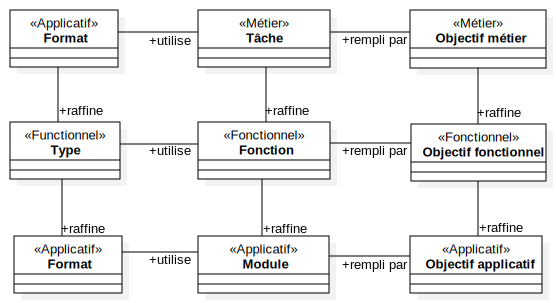
\includegraphics[trim= 0cm 18cm 0cm 0cm, clip, width=1\textwidth]{figures/4_demarche/metamodele_vue_integration.pdf}
    \caption{Métamodèle de la vue intégration}
    \label{fig:metamodele_vue_integration}
\end{figure}


Qu'il s’agisse d'une cohérence intra-vue ou inter-vues, la vue intégration définit un \textit{mapping} en spécifiant
(1)~les entités à aligner, (2)~les liens de cohérence entre ces éléments et (3) des transformations de modèle
associées à ces liens. Nous identifions plusieurs cas de figures où ces transformations de modèle s'avèrent commodes
dans le contexte de l'EA dans la section \ref{sec:executeea}. Parmi ces cas de figure nous citons, notamment,
l'automatisation du passage d'une vue à l'autre en utilisant une transformation de modèle pour générer le code
d'un module de la vue applicative à partir d'un modèle de fonction de la vue fonctionnelle.

\section[Le framework ExecuteEA]{Le \emph{framework} \emph{ExecuteEA}}
\label{sec:executeea}
    
    % framework = approche conceptuelle + structure logique (pour organiser et mettre en cohérence les modèles d'architecture  + outils et langages

    Une approche par points de vue est indispensable à l’appréhension des systèmes complexes car elle permet de séparer
    les préoccupations des parties prenantes dans des vues distinctes. Chaque vue traduit donc la perspective d'une partie-prenante.
    De nombreux \emph{frameworks} d'EA adoptent de ce fait une approche par points de vue. Cependant, les différentes préoccupations
    sont souvent traitées de manière séquentielle et plus ou moins indépendante des autres vues comme l'attestent
    S.~Kurpjuweit et R.~Winter~\cite{kurpjuweit2007viewpoint}.

    Nous proposons donc un \emph{framewok} d'EA permettant de traiter
    les différentes vues d'architecture de manière intégrée tout en permettant à l'architecture d'entreprise d'accompagner l'entreprise
    sur toute sa trajectoire.  Le métamodèle EAT-ME représente la pierre angulaire de ce \emph{framework}.
    Nous recourons en effet à la méta-modélisation pour unifier les différentes activités
    d'architecture —~documentation, analyse et conception~—
    en les inscrivant dans le cadre méthodologique et technologique offert par l'IDM.

    La vision unificatrice de l'IDM a pour \emph{leitmotiv} l'usage systématique de modèles productifs~\cite{2005unification}, c'est-à-dire
    de modèles \textbf{exécutables} \emph{versus} les modèles purement contemplatifs habituellement utilisés pour mener 
    les différentes activités d'EA~\cite{kulkarni2013modelling}. Nous avons donc choisi la dénomination \emph{Execute Enterprise Architecture} (\emph{ExecuteEA}) pour le \emph{framework} que nous présentons dans cette section.

    Le \emph{framework ExecuteEA} repose sur trois piliers~: (1)~une approche unificatrice pour la modélisation d'architecture d'entreprise,
    (2)~un cadre structurant orienté points de vue et (3)~l'identification d'un ensemble de langages et de techniques issus de l'IDM
    et adaptés à l'analyse d'architecture d'entreprise.



    % L'IDM prône en effet le recours systématique aux modèles productifs sur toute la chaine de production d'u 
    % Dans ces travaux de thèse, nous adoptons l'école de pensée \emph{Enterprise System Architecting} telle que définie
    % par Lapalme~\cite{lapalme2012three} et présenté dans le chapitre~\ref{ch:EA} traitant de l'état de l'art du domaine de l'EA.
    % De nombreux travaux ont démontré la capacité de l'IDM à traiter la complexité inhérente aux systèmes logicielles dont notamment
    % ceux de R. France et et B. Rumpe~\cite{france2007model}.


   \subsection{Approche conceptuelle et cadre structurant}

Parmi les différentes activités d'EA, nous avons choisi de focaliser nos travaux de thèse sur l'activité
d'analyse et ce pour plusieurs raisons.

D'abord, l'analyse fait partie des activités les moins traitées en EA~\cite{chen2008architectures}~\cite{barn2013enterprise},
quelle qu'en soit l'école de pensée comme relaté dans l'état 
de l'art concernant l'EA présenté au chapitre~\ref{ch:EA}. Cet état de fait est en partie dû
aux limitations des modèles contemplatifs qui font légion en EA. C'est pendant l'activité l'analyse que les modèles
exécutables sont le plus valorisés et indispensables.

Ensuite, comme l'illustre la figure~\ref{fig:activite_ea} l'analyse joue un rôle central dans une démarche d'EA.
Les modèles issus de l'analyse peuvent directement servir à documenter l'EA (\q{modèles EA validés} dans la figure~\ref{fig:activite_ea}).
Il s'agit de modèles qui recourent directement aux concepts du domaine de l'EA 
et qui ne nécessitent donc pas de changer de niveau d'abstraction pour être appréhendés par les parties prenants.
En IDM, ces modèles sont qualifiés de \emph{problem-level abstration models}~\cite{france2007model}.

\begin{figure}[!ht]
    \centering
    \includegraphics[width=1\textwidth]{figures/4_demarche/activite_ea.pdf}
    \caption{Évolution des modèles d'architecture \\
             et rôle central de l'activité d'analyse en EA}
    \label{fig:activite_ea}
\end{figure}

Enfin, l'analyse de modèles d'architecture est fortement liée à l'activité de conception. Le recours aux modèles
exécutables pour la conception d'architectures d'entreprise permet de mener des analyses directement sur ces
même modèles (\q{modèles EA à améliorer} et \q{modèles EA à valider} dans la figure~\ref{fig:activite_ea}). Dès lors que ces modèles sont validés à l'issue des activités d'analyse et de conception,
il devient possible de les utiliser pour la documentation (en mettant
automatiquement à jour les anciens modèles d'architecture) et pour l'implémentation. L'implémentation peut 
alors se faire par transformation de modèles, en transformant les \q{modèles EA validés} vers la plate-forme cible.

Nous entendons analyser deux aspects distincts mais corrélés d'une architecture
d'entreprise~: la structure et le comportement de la dite architecture.
L'analyse de la structure repose essentiellement sur la formalisation du métamodèle EAT-ME et vise à 
intégrer des modèles provenant des différentes vues d'architecture afin de garantir la cohérence
de l'ensemble de l'architecture. L'analyse du comportement de l'architecture repose quant à elle
essentiellement sur la simulation des modèles issus de l'analyse de la structure.
%Nous détaillons les activités l'analyse de la structure et du comportement dans la section~\ref{sec:analyse}.

\begin{figure}[!ht]
 \centering
 \includegraphics[trim= 0cm 2.5cm 0cm 0cm, clip, width=1\textwidth]{figures/4_demarche/approche_conceptuelle.pdf}
 \caption{Approche conceptuelle du \protect\emph{famework ExecuteEA}}
 \label{fig:approche_conceptuelle}
\end{figure}

Le \emph{framework ExecuteEA} englobe une approche conceptuelle et un cadre structurant les différentes activités d'EA, dont
notamment  l'analyse. Nous commençons par présenter l'approche conceptuelle illustrée par la figure~\ref{fig:approche_conceptuelle}.
L'approche consiste à définir un processus précis en identifiant
quatre rôles participant à ce processus~: l'architecte métier,
l'architecte fonctionnel, l'architecte applicatif et enfin l'architecte d'entreprise. Les trois premiers rôles ont déjà été présentés
dans la section~\ref{sec:roles}. 



Le processus commence par la modélisation de la vue métier par l'architecture
métier. L'architecte fonctionnel traduit la vue métier en une vue fonctionnelle 
en collaborant avec l'architecte
métier. L'architecte applicatif traduit la vue fonctionnelle en une vue applicative
tout en collaborant avec l'architecte fonctionnel et par extension avec l'architecte
métier. Le rôle de l'architecte d'entreprise consiste alors à orchestrer l'ensemble de ces
collaborations.

L'architecture ainsi modélisée est soumise à une analyse
structurelle menée par l'architecte d'entreprise en étroite collaboration avec
les architectes des différentes vues. L'architecte d'entreprise est alors
responsable de la vue intégration qui a pour mission de vérifier la cohérence
globale des modèles d'architecture. Ainsi intégrés, les modèles sont soumis à
une analyse comportementale via la simulation.
L'approche proposée suit un processus itératif. À l'issue de la simulation, l'ensemble des
architectes valident ou modifient leurs modèles selon les résultats de la simulation, et ainsi de
suite jusqu'à obtenir une architecture satisfaisante pour l'ensemble des parties prenantes.

\begin{figure}[!ht]
 \centering
 \includegraphics[trim= 0cm 2cm 0cm 2cm, clip, width=1\textwidth]{figures/4_demarche/vue_integration.pdf}
 \caption{Cadre structurant de \protect\emph{ExecuteEA}}
 \label{fig:cadre_structurant}
\end{figure}

L'approche proposée s'inscrit en outre dans un cadre structurant qui reprend les concepts identifiés dans le métamodèle
EAT-ME. Ce cadre est illustré par la figure~\ref{fig:cadre_structurant}. Ce cadre structure et organise les différents modèles
créés par les architectes~: métier, fonctionnel et applicatif. Chaque vue est en effet composée de trois aspects~: information,
processus et objectif. Notre contribution principale consiste à doter ce cadre d'une vue intégration transverse à toutes les autres vues.
Cette vue reflète la perspective de l'architecte d'entreprise qui a pour mission de garantir la cohérence globale de l'architecture,
et s'assure de l'alignement métier/IT. La vue intégration permet donc à l’architecte d'entreprise
d'expliciter les liens de cohérence intra-vue (\emph{via} les liens \q{remplit} et \q{utilise}) et inter-vues (via les liens de \q{raffinement}).




% Créer des modèles d'architecture d'entreprise qui sont appropriés à l'analyse des 
% modèles d'architecture implique de suivre un processus précis. 
% L'objectif de nos travaux est de définir le processus de modélisation approprié, les
% rôles impliqués, les artefacts conceptuels requis, ainsi que les outils et les
% langages adéquats pour mener des analyses de structure et de comportement.

% Notre contribution est double. Tout d'abord, nous proposons un frune démarche de
% modélisation et d'analyse qui s'appuie sur un cadre d'architecture multi-vues.
% Nous dotons ce cadre d'architecture d'une vue supplémentaire qui est la vue
% \textit{intégration}. Cette vue a pour but d'adresser les problématiques de
% cohérence et d'alignement. Ensuite, nous mettons à profit les langages et
% standards de l'IDM permettant de modéliser et de simuler les architectures
% d'entreprise.




% \begin{figure}[!ht]
%  \begin{center}
%  \includegraphics[trim= 0cm 13cm 0cm 2cm, width=1\textwidth]{figures/4_demarche/metamodele_framework.pdf} \end{center}
%  \caption{Métamodèle du framework proposé}
%  \label{fig:metamodele_framework}
% \end{figure}

% Nous donnons le métamodèle de la vue intégration dans la figure
% \ref{fig:metamodele_vue_integration}. Cette vue permet des vérifications
% horizontales à l'intérieur de chacune des vues. En effet, l'association
% «~utilise~» assure donc la compatibilité des données échangées entre les tâches
% d'un processus métier, les fonctions d'un bloc fonctionnel ou entre les modules
% d'une application (voir figure \ref{fig:metamodele_vue_integration}).
% L'association «~rempli par~» hérite aussi de la classe «~IntraVue~» et associe
% explicitement une entité à l'objectif qui lui est assigné. De cette manière, il
% est possible de tracer l'implémentation effective d'une stratégie métier à
% travers l'ensemble de l'entreprise, des entités métier à l'IT.




% Nous considérons donc que la documentation et la communication, l'analyse et la
% compréhension et enfin la conception et l'implémentation concernent tout le système entreprise et
% pas seulement sa composante SI. Par exemple, contrairement à une EA centrée sur
% les SI, les processus métier sont modélisés et évalués tout autant que
% l'architecture applicative. 



% L'analyste métier, l'architecte fonctionnel et l'architecte applicatif
% collaborent entre eux et avec l'architecture d'entreprise pendant tout le
% processus de modélisation. Par la suite, l'activité d'intégration incombe à
% l'architecte d'entreprise, détenteur de la vision globale. Mais l'intégration
% des vues implique de rebouclage avec les autres acteurs (analyste métier,
% architecte fonctionnel et architecte applicatif) pour garantir l'alignement
% business/IT. Les étapes de modélisation et d'intégration de notre approche
% répondent donc aux objectifs de conception et de communication tels que définis
% par Kurpjuweit et Winter~\cite{kurpjuweit2007viewpoint}.




    \subsection{Analyse de l'architecture d'entreprise}
    \label{sec:analyse}
Le cadre structurant et l'approche conceptuelle du \emph{framework ExecuteEA} permettent de mieux articuler entre elles les activités d'analyse de la structure et du comportement. L'analyse automatisée de ces modèles facilite leur appréhension par l'acteur qui
mène ces analyses (en l'occurrence l'architecte d'entreprise). Dans cette section, nous expliquons comment le recours aux modèles exécutables tel que préconisé par l'IDM permet de réaliser ces analyses.

    \subsubsection{Analyse de la structure}


L'analyse structurelle d'une architecture d'entreprise a plusieurs visées. Il peut s'agir de (1) la
vérification de la cohérence de l'ensemble de l'architecture (2) anticiper les changements en
en mesurant par exemple l'impact~\cite{de2005change} sur la structure de l'architecture.
Le métamodèle EAT-ME rend possible cette analyse en exploitant la relation de conformité qui lie un modèle à son
métamodèle telle que présentée dans l'état de l'art concernant les relations de base de l'IDM
au chapitre~\ref{ch:IDM}. 

La formalisation d'un métamodèle pour l'EA permet de plus de
contrôler la conformité des modèles d'architecture. En effet, le métamodèle
contraint les modèles d'architecture et offre la possibilité de vérifier
que l'ensemble des modèles respecte bien les contraintes exprimées par le
métamodèle.
Dans le cadre de EAT-ME, ces contraintes sont exprimées à travers les liens
de cohérence. Par exemple, toutes les entités de base (action, objectif et information)
doivent toujours appartenir à deux vues~: la vue intégration en plus d'une autre vue
parmi les vues métier, fonctionnelle, applicative et technique. Cette contrainte permet de vérifier
que toutes les entités de l'architecture sont bien répertoriées dans la vue intégration.

Autre exemple de contraintes exprimées dans le métamodèle EAT-ME~: tous les objectifs de la vue métier
doivent avoir des liens de cohérence inter-vues avec les objectifs de la vue fonctionnelle, et de même pour ces derniers
avec les objectifs de la vue applicative. Cette contrainte permet de vérifier que tous les objectifs exprimés par le métier sont bien pris
en compte par les applications de l'entreprise. Cette cohérence inter-vues est renforcée par une autre contrainte intra-vue
exprimée dans le métamodèle EAT-ME. Chaque action doit disposer d'un lien de traçabilité vers l'objectif qu'elle remplit.
Le croisement  de ces deux contraintes, exprimées au niveau du métamodèle, permet de vérifier que les modèles disposent
bien des liens de traçabilité nécessaire à la vérification de l'alignement métier/IT.

L'exploitation des contraintes exprimées sur
les liens de traçabilité de la vue intégration  permet de vérifier par exemple 
que toutes les tâches métier sont bien reliées aux fonctions
qui les réalisent, et que ces fonctions sont bien reliées aux modules applicatifs qui les implémentent.
L'analyse de cohérence permettra de vérifier que tous éléments de base de type action du  modèle
disposent bien de liens de traçabilité, et de les ajouter si nécessaire. Le même principe s'applique sur les
liens de traçabilité entre informations appartenant à différentes vues, auquel cas l'analyse permettra de vérifier que tous
les concepts métier disposent bien de liens vers leurs types dans la vue fonctionnelle, et vers leur format
dans la vue applicative.

L'analyse de la cohérence permet de plus d'identifier les transformations de modèle utiles à l'intégration de l'architecture.
Les transformations de modèle présentent en effet plusieurs atouts dans le contexte de l'IDM en général
et de l'EA en particulier. Supposons par exemple qu'il s'avère que
l'orchestration de deux modules est impossible à cause d'une incompatibilité de format
à l'issue de l'analyse de la cohérence de la structure. Dans ce cas, il est possible de créer une transformation
de modèle et de l'associer au lien de cohérence intra-vue dans la vue intégration. La figure~\ref{fig:transfo_coherence}
illustre ce principe dans le cas général d'une action et d'une information.

\begin{figure}[!ht]
 \centering
 \includegraphics[trim= 0cm 7.5cm 0cm 0cm, clip, width=1\textwidth]{figures/4_demarche/transfo_coherence.pdf}
 \caption{Identification d'une transformation de modèles \\
          pour garantir une cohérence intra-vue}
 \label{fig:transfo_coherence}
\end{figure}

La transformation de modèle est un moyen de renforcer l'alignement métier/IT en automatisant le passage d'une vue
à l'autre. Avec les technologies IDM actuelles, il est possible par exemple de transformer une fonction en un code pour
le module applicatif qui l'implémente. Le passage de la vue métier à la vue fonctionnelle demeure quant à lui essentiellement
manuel. L'analyse de la cohérence vise à identifier, dans la vue intégration, ce type de transformation de modèle
et les entités du modèle qu'il concerne.
Les transformations de modèle constituent une solution pour capitaliser le savoir faire métier au niveau des modèles et le rendre
plus indépendant de la plate-forme d'implémentation. Ainsi, il est possible de raisonner au niveau fonctionnel, en modifiant une fonction par exemple, et de réutiliser une transformation de modèle préalablement créée pour re-générer le code du module applicatif cible.

La vue d'intégration offre ainsi la possibilité d'analyser la cohérence de l'architecture d'entreprise
à travers la méta-modélisation, la relation de conformité de l'IDM et les transformations de modèle.
%À l'issue de l'analyse de la cohérence de la structure, l'architecture est 

Cette vue donne ainsi accès aux informations de traçabilité qui
permettent de déterminer l'impact d'une modification ou d'une défaillance d'un
module applicatif sur les processus métier. Elle permet aussi de vérifier que
les formats applicatifs permettent d'encoder les types de données fonctionnels
requis, qui eux-mêmes raffinent les concepts métiers. Cette vue détermine les
éventuelles transformations de modèle nécessaires au déploiement en spécialisant
l'association «~raffine~». Le choix des modèles à transformer dépend fortement
de leur nature (modèles graphiques, textuels, etc.) et mais aussi de leur niveau
d'abstraction. Par exemple, la génération de code demande un modèle en entrée
suffisamment détaillé pour exécuter une transformation pertinente. L'état de
l'art actuel des langages de transformation de modèle privilégie l'usage des
transformations de modèle entre la vue fonctionnelle et et la vue applicative.


Il est indispensable de s'assurer de la cohérence
entres les modèles des différentes vues avant d'initier une analyse
d'impact du changement qui soit pertinente pour les parties prenantes, en particulier
pour l'architecte d'entreprise. L'analyse de l'impact du
changement consiste à dévoiler les effets de bord d'un changement apporté à un
élément de l'architecture.

Dans le contexte du \q{framework ExecuteEA}, l'analyse d'impact exploite les
liens de traçabilité pour identifier les éléments du modèle impacté par une modification 
apportée à une entité du modèle d'architecture.
L'analyse d'impact évalue par exemple la conséquence de l'indisponibilité d'un module applicatif sur l'architecture
globale~: en mettant à profit les liens de cohérence de la vue intégration, il
est alors possible de déterminer quels sont les processus métier ou
fonctionnels touchés par cette défaillance applicative. De la même manière, il devient
possible d'identifier les modules applicatifs existants pouvant participer à la
réalisation d'un nouveau processus métier si ce processus fait intervenir des tâches
métier déjà implémentées dans le SI.

Nous proposons donc d'analyser les impacts en exprimant des requêtes sur les modèles
d'architecture et d'étudier le résultat de ces requêtes. Nous tirons profit des méthodes IDM telle la méta-modélisation en les
associant à des langages capables d'exprimer et d'exécuter des requêtes sur les modèles d'architecture,
tels que OCLinEcore ou QVT.


L'automatisation de l'analyse d'impact est particulièrement cruciale pour les grandes entreprises qui ont à gérer
un patrimoine applicatif important et un nombre de processus métier conséquent.
Il s'agit là d'une analyse statique, le raisonnement concerne uniquement l'aspect structurel. Nous abordons l'analyse
du comportement de la structure dans la suite de ce chapitre.

% Notre contribution consiste à définir la manière dont les langages et techniques
% de l'IDM peuvent être utilisés pour mener une analyse structurelle des modèles
% d'entreprise. Le cadre d'EA que nous proposons permet d'acquérir une vision
% globale et cohérente de l'ensemble des artefacts qui la composent. La taille de
% plus en plus importantes des entreprises actuelle fait que la complexité de
% l'entreprise en tant que système se retrouve dans les modèles d'architecture qui
% le représentent.



% Les langages de modélisation doivent donc permettre de représenter
% convenablement les différents composants de l'entreprise en plus d'offrir la
% possibilité d'analyser la structure des modèles créés dans l'objectif de mieux
% comprendre le système réel, qui est dans ce cas l'entreprise.  Grâce à ce type de langage
% il est possible de~:

% \begin{enumerate}
%     \item modéliser des règles de structure supplémentaires qui précisent d'avantage méta-modèle d'architecture. Une fois
% que le modèle d'architecture est conforme à ce métamodèle, il est possible de
% vérifier qu'il respecte bien toutes les contraintes exprimées au niveau du
% métamodèle~;
%     \item 
%     \end{enumerate}




        \subsubsection{Analyse du comportement : simulation dirigée par les processus
métier}

Comme relaté dans l'état de l'art, l'analyse fait partie des activités les moins
courantes de l'EA quelle qu'en soit l'école de pensée
\cite{chen2008architectures}~\cite{barn2013enterprise}. Et même lorsqu'une
architecture d'entreprise est analysée, très peu d'approches recourent à la
simulation pour analyser l'aspect comportemental~\cite{glazner2011enterprise}
\cite{manzur2015xarchimate}. La simulation est pourtant une technique reconnue
pour évaluer le comportement d'un système et/ou évaluer plusieurs stratégies
concernant son fonctionnement~\cite{shannon1975systems}. Notre approche
préconise de simuler les modèles issus des activités de modélisation et
d'intégration afin de les valider ou les critiquer par l'ensemble des acteurs
impliqués dans l'EA.

Pour simuler le comportement d'une entreprise nous nous appuyons sur les modèles
d'architecture d'entreprise préalablement définis par les différentes parties
prenantes. L'EA permet de capturer l'essentiel des composants d'une
entreprise sous forme d'abstractions. Une approche par points de vue guide la
décomposition d'une entreprise en vues pertinentes pour les différents acteurs.
Ces vues apportent une aide supplémentaire à la définition du périmètre des
modèles de simulation. La vue intégration permet en particulier de définir les
liens entres les différentes vues, donc entre les différents modèles de
simulation et de garantir la cohérence et donc la pertinence de la simulation.
Comme les modèles de simulation sont directement dérivés de l'architecture
d'entreprise telle qu'elle est définie par les parties prenantes, elle est
d'autant plus facile à appréhender. Ces derniers peuvent aussi
aisément communiquer et échanger autour des résultats de la simulation.

Les modèles d'entreprise doivent offrir un niveau d'abstraction suffisant à la
compréhension, l'analyse et la communication. Les modèles doivent donc permettre
d'abstraire les détails techniques et les nombreuses interconnexions tout en
garantissant la traçabilité et la cohérence de l'ensemble de l'architecture.
Notre approche consiste donc à mettre en lumière les composants et les
relations qui sont critiques pour le comportement de l'ensemble de
l'architecture. En effet, modéliser l'architecture d'une entreprise revient à la
modélisation de systèmes complexes. Herbert Simon~\cite{simon1990prediction}
dans ses travaux de modélisation de systèmes complexes affirme que
«~l'approximation judicieuse et non la puissance de calcul d'une machine~» reste
la manière la plus effective d'adresser des systèmes complexes.

La simulation des processus métier est souvent réduite à de la simple animation
visuelle de diagrammes pour vérifier l'orchestration des tâches métier. Nous
proposons de piloter la simulation du comportement de l'architecture par le
processus métier. Dans ce cas, le calcul d'une valeur ne se fait pas au niveau
de la tâche métier, mais au niveau du module applicatif qui l'implémente. Le processus
métier est modélisé sous forme de diagrammes d'activité fUML. Dans ce cas, la
simulation du comportement de l'architecture d'entreprise est pilotée par les
processus métier qui sont alors responsables d'orchestrer l'ensemble des modèles
comme l'illustre la figure \ref{fig:Simulation_Approche}. 

La simulation est
lancée après l'intégration de l'architecture à travers la création de liens de
cohérences intra-vue et inter-vues. Ces liens sont par la suite utilisés pour
mettre en œuvre la simulation. D'une part, la \textit{Tâche~A} de la figure
\ref{fig:Simulation_Approche} appelle le \textit{Module~A} car le
\textit{Module~A} raffine la \textit{Fonction~A} qui elle-même raffine la
\textit{Tâche~A}. D'autre part, les liens de cohérences intra-vue garantissent une
compatibilité entre les informations envoyées par la \textit{Tâche~A} et celles
attendues par la \textit{Tâche~B}, de même entre la \textit{Fonction~A} et la
\textit{Fonction~B} et entre le \textit{Module~A} et le \textit{Module~B}.

\begin{figure}[!ht]
    \centering
    \includegraphics[trim= 0cm 1cm 0cm 1cm, clip, width=1\textwidth]{figures/4_demarche/approche_simulation.pdf}
    \caption{Simulation de l'architecture dirigée par les processus}
    \label{fig:Simulation_Approche}
\end{figure}

En plus de s'appuyer sur les processus métier pour piloter la simulation de
l'ensemble du comportement de l'architecture d'entreprise, notre approche
consiste à mettre à profit les techniques et les langages de l'IDM pour
faciliter l'automatisation de l'activité d'analyse du comportement. Nous nous
appuyons sur le manifeste de IBM~\cite{chesbrough2006research} concernant l'IDM
dans la sélection de techniques et langages qui soient pertinents pour notre
approche. Le manifeste de IBM recommande l'utilisation de langages
(1)~exécutables, (2)~standardisés et (3)~compréhensibles par les experts du
domaine. C'est le cas de fUML, BPMN et OCL. La table~\ref{fig:IDM_EA} fait la
correspondance entre les langages et la possibilité de les utiliser selon les
vues.

\begin{table}[!ht]
    \centering
    \setlength{\mytablewidth}{0.8\textwidth}
\setlength{\mycolwidth}{\dimexpr0.25\mytablewidth-2\tabcolsep\relax}

\begin{tabulary}{\mytablewidth}{m{\mycolwidth}m{\mycolwidth}m{\mycolwidth}m{\mycolwidth}}
\cmidrule[\heavyrulewidth]{2-4}

                        & \centbf{Metier}       & \centbf{Fonctionnel}  & \centbf{Applicatif}   \tabularnewline\midrule
    \centbf{BPMN}       & \center{\checkmark}   &                       &                       \tabularnewline
    \centbf{fUML}       & \center{\checkmark}   & \center{\checkmark}   &                       \tabularnewline
    \centbf{OCL}        &                       & \center{\checkmark}   &                       \tabularnewline
    \centbf{MiniZinc}   &                       &                       & \center{\checkmark}   \tabularnewline

\bottomrule
\end{tabulary}

    \caption{Langages de l'IDM pour l'EA}
    \label{fig:IDM_EA}
\end{table}


Ces langages permettent une exécution directe des modèles créés, contrairement à
d'autres méthodes de simulation de processus métier qui utilisent l'IDM pour
isoler la définition du processus de son exécution. Ces méthodes font ensuite
appel aux transformations de modèle pour automatiser la conversion entre les
modèles de représentation et leur exécution.

\section{Conclusion}

Dans ce chapitre, nous avons présenté un \emph{framework} offrant un cadre structurant et unificateur 
pour les différentes activités d'EA. Ce \emph{framework}, appelé ExecuteEA, permet d'automatiser
l'analyse structurelle et comportementale d'une architecture d'entreprise. 

L'analyse structurelle
s'appuie sur l'exploitation des liens de traçabilité du métamodèle EAT-ME. Ce métamodèle
explicite en effet des liens de cohérence intra-vue et inter-vues reliant les différents composants
d'une architecture d'entreprise. 

Nous avons proposé, pour l'analyse comportementale, une approche
de simulation d'architecture dirigée par les processus métier. La simulation est rendue possible par
le recours aux transformations de modèle et aux langages de modélisation exécutable.

La définition du métamodèle EAT-ME a nécessité une analyse du domaine de l'EA en général, et dans le
contexte des Smart Grids en particulier, conformément à la démarche préconisée par l'IDM.  

Dans le chapitre suivant, nous décrivons une implémentation du \emph{framework} ExecuteEA que nous
éprouvons sur le cas métier d'une gestion de flotte de véhicules électriques.



















% \begin{figure}[!ht]
%     \begin{center}
%     \includegraphics[trim= 0cm 3cm 0cm 0cm, width=1\textwidth]{figures/4_demarche/vue_aspect.pdf}
%     \end{center}
%     \caption{Points de vue et aspects utilisés} \label{fig:vue_aspect}
% \end{figure}

% Nous
% préconisons l'utilisation de formalismes standards pour la modélisation de
% processus métier qui soient exécutables, tels que les diagrammes d'activité \gls{fuml} 
% ou les diagrammes \gls{bpmn} dans une perspective de simulation. Des langages
% spécifiques à un domaine (\gls{dsml}) peuvent également être utilisés~;






    %!TEX  root = main.tex
\chapter{Prototypage et validation du \emph{framework ExecuteEA}}
\label{ch:implem}

\PartialToc


\section{Environnement retenu : la plate-forme Eclipse}

Notre choix s'est orienté vers la plate-forme Eclipse et ce pour plusieurs
raisons.

Tout d'abord, il s'agit d'une plate-forme open-source dont l'utilisation est
particulièrement répandue dans la communauté IDM. En effet, la plate-forme
Eclipse abrite le projet
\gls{emf}\footnote{http://www.eclipse.org/modeling/emf/} qui a pour objectif de
doter Eclipse d'outils orientés IDM.

Ensuite, \gls{emf} s'appuit sur les standards du domaine. Par exemple, le méta-
métamodèle Ecore, pilier central de \gls{emf}, se base sur le standard
\gls{mof}\footnote{http://www.omg.org/mof/} . Aure exemple, le langage de
contraintes OCLinEcore se base sur le standard \gls{ocl}. OCL et MOF sont des
standard de l'OMG.

Puis, \gls{emf} se décompose en sous-projets orientés vers différents aspects de
l'IDM tels que la méta-modélisation, la transformation de modèle, les éditeurs
graphiques de modèles, les langages spécifiques au domaine. \gls{emf} offre
ainsi un environnement personnalisable pour mettre en œuvre une approche IDM.

Enfin, il s'agit de la plate-forme retenu par le projet Pomme du département
MIRE, dans lequel s'inscrit nos travaux de thèse. Le projet Pomme vise à
réaliser un outil pour la co-simulation des trois domaines qui compose un Smart
Grid~: SI, infrastructure électrique, infrastructure de télécommunication.

Pour ces travaux de thèse, nous avons donc retenu~:

\begin{itemize}

    \item Ecore pour la méta-modélisation~;

    \item OCLinEcore pour l'expression de contraintes et de requêtes sur le métamodèle~;

    \item Le langage Acceleo pour les transformations de modèle~;

    \item Le plugin Papyrus\footnote{https://eclipse.org/papyrus/} pour la simulation
    des modèles d'architecture. Papyrus est compatible avec le standard fUML et
    permet donc d'exécuter les diagrammes de classes et d'activité. 

\end{itemize}


\section{Réalisation et difficultés rencontrées}

    \subsection{Implémentation du métamodèle EA2M avec Eclipse Modeling Framework}

    Le métamodèle EA2M est le pilier central du \emph{framework ExecuteEA}. Nous
    l'avons implémenté à l'aide de \gls{emf}. Il est donc conforme au méta-
    métamodèle Ecore. EMF génère automatiquement un éditeur de modèle à partir
    d'un métamodèle conforme à Ecore. Cet éditeur permet de créer des modèles
    d'architecture d'entreprise conformes au métamodèle EA2M ainsi implémenté.
    La figure~\ref{fig:editeur_modele1} et la figure~\ref{fig:editeur_modele2}
    sont une capture d'écran de l'éditeur de modèles générée automatiquement à
    partir du métamodèle EA2M. L'utilisateur a le choix de créer une vue métier,
    fonctionnelle, applicative ou intégration et pour chacune des vues il peut
    choisir de créer un aspect objectif, processus ou information.


    \begin{figure}[!htbp]
     \begin{center}
      \includegraphics[width=0.8\textwidth]{figures/5_implementation/editeur_modele1.png}
     \end{center}
     \caption{Edition de modèles d'architecture d'entreprise avec ExecuteEA\\création de vues}
     \label{fig:editeur_modele1}
    \end{figure}

    \begin{figure}[!htbp]
     \begin{center}
      \includegraphics[width=0.8\textwidth]{figures/5_implementation/editeur_modele2.png}
     \end{center}
     \caption{Edition de modèles d'architecture d'entreprise avec ExecuteEA\\création d'aspects}
     \label{fig:editeur_modele2}
    \end{figure}

    La figure~\ref{fig:modeleEA} représente une capture d'écran d'un modèle d'architecture
    d'entreprise créé avec l'éditeur de modèle ExecuteEA.

    \begin{figure}[!htbp]
     \begin{center}
      \includegraphics[trim=0cm 3cm 0cm 0cm, width=0.8\textwidth]{figures/5_implementation/modele_ea.pdf}
     \end{center}
     \caption{Modèle d'architecture d'entreprise créé avec l'éditeur ExecuteEA}
     \label{fig:modeleEA}
    \end{figure}

    La difficulté majeure rencontrée en implémentant le métamodèle EA2M a été de
    trouver le bon équilibre entre deux impératifs~: (1) implémenter le
    métamodèle en utilisant des concepts et des relations qui font sens d'un
    point de vue EA, en se gardant la possibilité de l'étendre facilement,
    notamment, par d'autres aspects ou d'autres vues, (2) tout en créant un
    éditeur suffisamment contraignant pour créer des modèles d'architecture
    corrects. Par exemple, utiliser uniquement le mécanisme de multiplicités
    entre la classe abstraite \q{Vue} et la classe \q{Architecture} ne contraint
    pas le modélisateur à ne pas créer plusieurs fois le même type de vue pour
    une seule architecture. Un modèle avec deux vues métier serait par
    conséquent conforme au métamodèle mais ne serait pas pertinent d'un point de
    vue EA.

    Nous avons donc exprimé des contraintes avec OCLinEcore pour ne créer que
    des modèles pertinents tout en gardant un métamodèle pertinent d'un point de
    vue purement EA.  Une contrainte est une expression à valeur booléenne qui
    sert à préciser ou restreindre n'importe quel élément du métamodèle.

    La figure~\ref{fig:contraintes_ocl_architecture} illustre le métamodèle
    EA2M, implémenté à l'aide d'\gls{emf}, sous une forme textuelle\footnote{EMF
    est doté d'une éditeur graphique qui permet de créer des métamodèles de
    manière graphique (par \emph{drag and drop}) sous la forme d'un diagramme de
    classe et de générer le même métamodèle sous une forme textuelle.}. Il
    s'agit donc de la classe \q{Architecture} à la quelle on a ajouté des
    contraintes de type \q{invariant} pour qu'elle ne contiennent pas de vue du
    même type.

    \begin{figure}[!htbp]
     \begin{center}
      \includegraphics[width=0.8\textwidth]{figures/5_implementation/ocl_in_ecore_vue.png}
     \end{center}
     \caption{Contraintes OCLinEcore attachées à la classe \protect\q{Architecture} }
     \label{fig:contraintes_ocl_architecture}
    \end{figure}

    \subsection{Exécution des modèles d’architecture avec Papyrus}
    \label{sec:opaque_action_papyrus}

    Papyrus est un atelier de modélisation orienté IDM doté d'un moteur
    d'exécution de diagrammes fUML conformément aux spécifications de l'OMG.
    Nous l'avons utilisé pour simuler l'architecture. Comme présenté dans le
    chapitre~\ref{ch:proposition}, nous proposons de simuler l'ensemble de
    l'architecture en la pilotant par les modèles.  La difficulté majeure
    rencontrée à cette étape de l'implémentation a été de réussir à exécuter des
    comportements difficile à modéliser avec un diagramme
    UML\footnote{Typiquement, l'optimisation d'une affectation de véhicules
    électriques à des tournées d'agents qui intervient dans le cas d'études
    présenté dans la suite de ce chapitre}. Le principe de simulation pilotée
    par les processus métier, tel que présenté dans la
    figure~\ref{fig:Simulation_Approche}
    (page~\pageref{fig:Simulation_Approche}), exige de plus de faire appel aux
    modules de la vue applicative.
    
    Le standard fUML a prévu l'exécution de comportements spécifiques difficiles
    à modéliser avec  des diagrammes d'activité. Il dédie à cet effet une
    action\footnote{Dans les spécifications d'UML et de fUML, une action est une étape
    unitaire à l'intérieur d'une activité. Une activité est donc composée de
    plusieurs actions.} spécialisée~: l'\emph{OpaqueAction}. Papyrus s'appuie
    sur le moteur d'exécution Moka pour simuler les diagramme fUML. Moka est
    conforme à la sémantique d'exécution spécifiée par l'OMG pour fUML. Or la
    sémantique d'exécution de l'\emph{OpaqueAction} n'a pas encore été
    spécifiée. Le standard fUML est en effet relativement récent\footnote{La
    première version de fUML a été publiée par l'OMG en févier 2011} et n'a pas
    encore été entièrement spécifié. Pour cette raison, le moteur d'exécution
    Moka ne prend pas en charge l'exécution de l'\emph{OpaqueAction}

    Cependant, Papyrus donne la possibilité d'étendre le moteur d'exécution Moka
    et en attribuant le comportement souhaité à \emph{OpaqueAction} et en
    l'exécutant comme les autres actions au cours d'une simulation de diagramme
    d'activité. Cette extension n'a toutefois pas été facile à implémenter. Les
    tutoriels mis à disposition par l'équipe de développement du module Moka
    sont utiles pour une utilisation basique mais ne répondent à des besoins
    d'utilisation pointues telle que l'extension du moteur d'exécution
    disponible. À cet effet, nous avons sollicité l'aide de contributeurs au
    développement du module Moka et nous nous sommes également appuyé sur un
    stagiaire en dernière école d'ingénieur. Le comportement de
    l'\emph{OpaqueAction} mis en œuvre dans ces travaux de thèse consiste donc à
    appeler un module extérieur durant l'exécution d'un diagramme d'activité
    fUML et à retourner le résultat fourni par le module à l'action ou
    l'activité suivante.

    Dans la suite de ce chapitre, nous éprouvant le \emph{framework ExecuteEA}
    ainsi doté d'un environnement de modélisation et de simulation de modèles
    d'architecture. La validation est faite à travers le cas d'étude de la
    gestion d'une flotte de véhicules électrique. Nous avons créé à cet effet
    (1) les modèles d'architecture d'entreprise requis par les différentes vues
    et selon les aspects spécifié par \emph{ExecuteEA} en adoptant les langages
    prescrit par le \emph{framework}, et (2) les transformations de modèle
    nécessaires. Nous avons ensuite analyser l'architecture obtenue.


\section{Concrétisation de l'approche avec un cas d'étude}

    Les contraintes de temps et de confidentialité ne nous ont pas permis
    d'éprouvé le framework ExecuteEA sur une architecture d'entreprise à taille
    réelle. Pour cette raison, le cas d'étude concerne plutôt un seul processus
    métier faisant intervenir plusieurs tâches et sa déclinaison sur les vues
    fonctionnelle et applicative. Il s'agit de la gestion d'une flotte de
    véhicules électriques. Ce cas métier nous permet néanmoins de concrétiser
    les propositions de ces travaux de thèse et de parer à la difficulté
    d'évaluer quantitativement ces propositions.

    \subsection{Présentation du cas d'étude~:\\la gestion d'une flotte de véhicules électriques}

    Les raisons motivant le choix de ce cas d'étude pour éprouver le framework
    proposé dans ces travaux de thèse ont été discutées dans le
    section~\ref{motivations_cas_metier} (voir
    page~\pageref{motivations_cas_metier}).  Dans cette partie, nous nous
    contentons donc simplement de le présenter.

    Il s'agit du processus d'affectation de véhicules à des tournées d'agents
    (par exemple, une tournée d'un agent EDF qui relève les compteurs chez les
    client, ou encore qui fait des réparations le réseau électrique).  La
    mobilité électrique implique un changement de paradigme pour le gestionnaire
    de flotte de l'entreprise. D'une part, le véhicule électrique est limité par
    son autonomie et ne peut donc pas effectuer n'importe quelle tournée.
    D'autre part, la recharge d'un véhicule électrique implique des contraintes
    (temps de recharge, disponibilité des bornes) que ne présente pas le
    véhicule thermique qui se contente d'un plein de carburant.
    
    Dès lors, le processus d'affectation de véhicules aux tournées des agents,
    la gestion de la flotte de véhicules dans son ensemble et donc le SI qui
    l'implante sont fortement impactés par l'arrivée massive des véhicules
    électriques. Nous proposons de modéliser de cas d'étude selon en mettant en
    œuvre le \emph{framework ExecuteEA}. Nous adoptons donc l'approche
    conceptuelle préconisée par le framework (voir
    figure~\ref{fig:approche_conceptuelle},
    \pageref{fig:approche_conceptuelle}). Nous commençons donc par modéliser des
    différentes vues d'architecture —~métier, fonctionnelle, applicative et
    intégration~— en respectant le cadre structurant du \emph{framework
    ExecuteEA} (illustré par la figure~\ref{fig:cadre_structurant},
    page~\pageref{fig:cadre_structurant}) ce qui nous permettra ensuite
    d'analyser la structure et le comportement de l'architecture ainsi obtenue.

    \begin{figure}[!htbp]
     \begin{center}
      \includegraphics[trim=0cm 3cm 0cm 0cm, width=0.8\textwidth]{figures/5_implementation/processus_metier.pdf}
     \end{center}
     \caption{Processus d'affectation de véhicules électriques à des tournées}
     \label{fig:processus_metier}
    \end{figure}

    Pour ce cas d'étude, l'analyse de la structure exploite les liens de la vue
    intégration et la conformité du modèles d'architecture au métamodèle EA2M.
    L'analyse du comportement consiste à simuler l'ensemble de l'architecture en
    pilotant la simulation par le processus métier. Cette simulation a pour
    objectif de valider et critiquer  les choix de modélisation et d'anticiper
    l'éventuel dimensionnement de la flotte. Par exemple, si une forte
    proportion des tournées implique une distance effectuée supérieure à
    l'autonomie des véhicules électriques sans possibilité de recharge en cours
    de route (pas de borne à disposition au cours de la tournée), la simulation
    permet  de trouver la proportion de véhicules thermiques à garder a minima
    dans une flotte. L'affectation doit aussi privilégier l'utilisation des
    véhicules électriques car la rentabilité d'un parc de véhicules électriques
    est proportionnelle au nombre de kilomètres effectués par ces véhicules.

    \subsection{Mise en œuvre du \emph{framework ExecuteEA}\\
    pour la modélisation des vues métier, fonctionnelle et applicative}

    La première étape consiste donc à créer les modèles des vues métier, fonctionnelle
    et applicative en recourant à des langages de modélisation exécutables. Selon les
    propositions de ces travaux de thèse, l'usage de ces langages automatisent
    la manipulation des modèles et facilitent leur analyse. La
    figure~\ref{fig:architecture_generale_usecase} présente l'architecture \emph{in globo}
    du cas métier ainsi modélisé, selon le cadre structurant \emph{ExecuteEA}.






% Nous éprouvons notre démarche au cas métier de la gestion d'une flotte de
% véhicules électriques. Nous construisons les modèles adéquats pour les vues
% métier, fonctionnelle et applicative en adoptant des langages exécutables. La
% cohérence est modélisée dans la vue intégration. L'architecture globale du cas
% métier est illustrée dans la \ref{fig:architecture_generale_usecase}.


\begin{figure}[!htbp]
 \begin{center}
  \includegraphics[angle=90, width=1\textwidth]{figures/5_implementation/architecture_generale_usecase.pdf}
 \end{center}
 \caption{Architecture globale du cas d'étude \\mettant en œuvre le \protect\emph{framework ExecuteEA}}
 \label{fig:architecture_generale_usecase}
\end{figure}


\subsubsection{Modélisation de la vue métier} 

Nous utilisons fUML comme langage
exécutable pour modéliser cette vue. Le processus métier consiste à collecter
les données relatives aux véhicules (électriques et thermiques) ainsi qu'aux
tournées à effectuer, de calculer l'énergie nécessaire à chaque tournée et
l'affectation véhicule/tournée avant de faire valider cette dernière par le
manager de flotte. Nous modélisons ce processus métier sous forme de diagramme
d'activité fUML en utilisant l'atelier de modélisation Papyrus. Selon notre cadre
d'architecture, les modèles créés représentent donc l'aspect processus de la vue
métier. La figure~\ref{fig:processus_fuml} présente le diagramme d'activité fUML obtenu à
l'aide de Papyrus.

\begin{figure}[!htbp]
 \begin{center}
  \includegraphics[width=1\textwidth]{figures/5_implementation/processus_fuml.png}
 \end{center}
 \caption{Aspect processus de la vue métier modélisé sous la forme d'un diagramme d'activité fUML avec Papyrus}
 \label{fig:processus_fuml}
\end{figure}


Pour l'aspect information, nous utilisons des diagrammes de classe UML pour
représenter les concepts métier et leurs relations. Nous modélisons ainsi les
concepts de Véhicule, Tournée et Affectation. La figure~\ref{fig:information_metier}
présente le diagramme de classes fUML modélisé dans Papyrus.

\begin{figure}[!htbp]
 \begin{center}
  \includegraphics[width=1\textwidth]{figures/5_implementation/information_metier.png}
 \end{center}
 \caption{Aspect information de la vue métier modélisé sous la forme d'un diagramme de classes fUML avec Papyrus}
 \label{fig:information_metier}
\end{figure}

Gérer une flotte de véhicules peut
avoir plusieurs objectifs métier. Dans notre cas, obtenir le meilleur retour sur
investissement suite à l'intégration de véhicules électriques dans la flotte de
véhicules. Nous modélisons l'objectif métier sous la forme d'une classe UML
représentant l'aspect objectif de la vue métier comme l'illustre la 
figure~\ref{fig:architecture_generale_usecase}.

% Le choix des langages de modélisation et de l'outil de simulation est motivé par
% les pratiques du domaine. En effet, la Commission Électrique Internationale a
% adopté Enterprise Architect comme outil pour maintenir et distribuer le
% CIM\footnote{Common Information Model}\cite{uslar2012standardization}, un modèle
% d'information commun pour le domaine électrique
% \footnote{www.sparxsystems.com.au/press/articles/iec.html}.
	

\subsubsection{Modélisation de la vue fonctionnelle}

Nous modélisons l'aspect information de la vue fonctionnelle sous la forme d'un diagramme de classes
fUML. Ce modèle raffine les concepts métier en spécifiant leurs types. Dans la
vue fonctionnelle, le concept d'allocation prend la forme d'une association
entre les véhicules et les tournées. 

\begin{figure}[!htbp]
 \begin{center}
  \includegraphics[width=1\textwidth]{figures/5_implementation/information_fonctionnelle.png}
 \end{center}
 \caption{Aspect information de la vue fonctionnelle modélisé sous la forme d'un diagramme de classes fUML avec Papyrus}
 \label{fig:information_fonctionnelle}
\end{figure}

L'objectif fonctionnel est d'optimiser
l'utilisation des véhicules électriques pour atteindre l'objectif métier qui est
d'avoir un meilleur retour sur investissement. Nous modélisons cet objectif 
sous la forme d'une classe UML
représentant l'aspect objectif de la vue fonctionnelle comme l'illustre la 
figure~\ref{fig:architecture_generale_usecase}.

Pour l'aspect processus de la vue fonctionnelle, nous commençons par identifier trois blocs fonctionnels~:
un bloc pour la gestion de la flotte de véhicules (électriques et thermiques),
un bloc pour la gestion des tournées, un bloc pour la gestion de l'affectation
(voir figure \ref{fig:architecture_generale_usecase}. Ces blocs contiennent les
fonctions qui raffinent les tâches du processus métier. Comme expliqué plus tôt
dans la démarche, le fait de les rassembler dans des blocs selon les concepts
métier augmente la modularité et l'évoluvilité de l'architecture. De plus, nous
consacrons un bloc à la gestion des processus fonctionnels. Ce bloc est
responsable de l'orchestration des fonctions du processus fonctionnel.

Les blocs fonctionnels offrent une vue plus détaillée des tâches métier. 
Pour ce cas d'étude, nous détaillons uniquement la tâche métier qui consiste à
affecter un véhicule à une tournée. Nous modélisons l'affectation des véhicules 
aux tournées
sous la forme de contraintes \gls{ocl}~: pour affecter un véhicule à une tournée, il
faut que l'énergie nécessaire à celle-ci soit inférieure à l'autonomie de la
batterie. Dans notre cas d'application, nous considérons qu'il n'est pas
possible de recharge le véhicule pendant la tournée de l'agent.

Nous modélisons la fonction d'affectation sous la
forme de deux contraintes et d'une requête en utilisant OCL. La première contrainte OCL signifie
que si un véhicule électrique est affecté à une tournée alors l'énergie dont il
dispose permet d'assurer la totalité de la tournée. La deuxième contrainte
signifie que si aucun véhicule électrique n'est capable d'assurer une tournée
donnée alors c'est un véhicule thermique qui lui est associé. Enfin, la requête
calcule le nombre total de kilomètres électriques correspondant à la distance
parcourue par les véhicules électrique après l'affectation. Cette requête permet
d'évaluer l'utilisation  des véhicules électriques dans l'optique d'atteindre
l'objectif fonctionnel.

Il est possible de modéliser les autres algorithmes de
traitement (calcul des tournées à partir de bon de travaux, calcul de l'énergie
nécessaire à une tournée, etc.) à l'aide de diagrammes d'activité exécutables.



\lstinputlisting[caption=Contraintes OCL pour la fonction d'affectation]{figures/5_implementation/tournee.ocl}

\subsubsection{Modélisation de la vue applicative}

Pour les processus applicatifs, nous commençons par identifier  les applications
nécessaires à l'implantation des blocs fonctionnels. Dans notre cas, le
patrimoine applicatif de l'entreprise dispose déjà d'applications pour la
gestion de tournées (calcul de tournées optimisé à partir de bons de travaux) et
la gestion de véhicules (administration, maintenance, etc.). Pour la fonction
d'allocation, nous faisons le choix d'utiliser MiniZinc pour modéliser les
contraintes au niveau applicatif \ref{fig:contraintesMiniZinc}.

\begin{figure}[!htbp]
 \begin{center}
  \includegraphics[width=1\textwidth]{figures/5_implementation/module_minizinc.png}
 \end{center}
 \caption{Contraintes du module MiniZinc}
 \label{fig:contraintesMiniZinc}
\end{figure} 

MiniZinc est un langage de modélisation et de résolution de contraintes de
niveau intermédiaire qui a pour vocation de devenir un langage de modélisation
standard dans le domaine de la programmation par contraintes. L'aspect
information contient les formats de données nécessaires aux différentes
applications. La figure \ref{fig:formatMiniZinc} représente le fichier de
données (le format .dzn) nécessaire à l'application MiniZinc pour calculer
l'affectation.

\begin{figure}[!htbp]
 \begin{center}
  \includegraphics[width=0.5\textwidth]{figures/5_implementation/format_minizinc.png}
 \end{center}
 \caption{Fichier de données pour le module MiniZinc}
 \label{fig:formatMiniZinc}
\end{figure} 

Nous modélisons l'objectif applicatif sous la forme d'une classe UML
représentant l'aspect objectif de la vue applicative comme l'illustre la
figure~\ref{fig:architecture_generale_usecase}. Un véhicule électrique devient
rentable par rapport à un véhicule thermique à partir d'un certain nombre de
kilomètre parcouru. C'est pourquoi l'objectif fonctionnel qui est d'optimiser
l'usage de la flotte électrique se traduit par la maximisation du nombre de
kilomètres électriques, c'est à dire affecter aussi souvent que possible un
véhicule électrique aux tournées. Ainsi, le module MiniZinc prend en compte cet
objectif en résolvant les contraintes tout en maximisant la distance électrique.



\subsection{Intégration et analyse de la structure}

L'approche conceptuelle que nous proposons pour le \emph{framework ExecuteEA},
illustrée par la figure~\ref{fig:approche_conceptuelle} à la
page~\pageref{fig:approche_conceptuelle}, met l'accent sur le rôle intégrateur
de l'architecte d'entreprise~: il doit s'assurer de la cohérence intra-vue et
inter-vues de l'architecture globale tout en collaborant avec les architectes
métier, fonctionnel et applicatif.

L'intégration de l'architecture passe par la modélisation de la vue intégration,
c'est-à-dire par la spécification des liens de cohérence  intra-vue et et inter-
vues conformément au métamodèle EA2M. Nous avons donc modélisé ces liens pour
l'ensemble des vues métier, fonctionnelle et applicative. Néanmoins, la figure
\ref{fig:integration_gestion_flotte} ne présente qu'une partie modèles
d'intégration pour des raisons de lisibilité. Nous y modélisons à titre
d'illustration les liens de cohérence intra-vue entre la fonction d'affection,
ses inputs et output en termes de types fonctionnels, ainsi que son objectif
fonctionnel. Nous faisons de même pour le module d'optimisation MiniZinc, ses
inputs et outputs ainsi que l'objectif applicatif qu'il remplit. Le même
principe d'intégration intra-vue, c'est à dire entre les aspects d'une même vue,
est applicable à tous les autres éléments de la vue métier, fonctionnelle et
applicative.

\begin{figure}[!htbp]
 \begin{center}
  \includegraphics[trim= 0cm 0cm 0cm 0cm, width=1\textwidth]{figures/5_implementation/integration_affectation.pdf}
 \end{center}
 \caption{Une vue partielle des modèles d'intégration \\de la vue fonctionnelle et de la vue applicative}
 \label{fig:integration_gestion_flotte}
\end{figure}

De la même manière, nous modélisons les liens de cohérence inter-vues. Par
exemple, le lien \q{consomme} exprime qu'un type de données est compatible avec
la fonction qui l'utilise et qu'un format est compatible avec le module
applicatif qui l'utilise en entrée. Pour garantir une bonne orchestration des
processus, il faut que le \q{produit} d'une tâche (respectivement une fonction,
un module applicatif) soit compatible avec le ce que produit la tâche suivante
(respectivement une fonction, un module applicatif).

L'intégration passe aussi par l'identification des éventuelles transformation de
modèles. Rappelons ici que les transformations ont pour objectif d'améliorer
l'alignement métier/IT en automatisant le passage d'une vue à une autre. Pour le
cas métier de la gestion de flotte de véhicules, nous utilisons une
transformation de modèle pour générer les contraintes pour le module de calcul
d'affectation MiniZinc de la vue applicative à partir des contraintes OCL
exprimées dans la fonction affectation de la vue fonctionnelle. La
transformation est écrite dans le langage de transformation Acceleo. En plus de
transformer les contraintes décrite dans l'aspect métier, cette transformation
de modèle permet aussi de transformer les instances des types fonctionnels en
instances dans le format \q{.dzn} utilisé par le module MiniZinc comme
l'illustre la figure \ref{fig:integration_gestion_flotte}. La génération de code
pour le module MiniZinc peut être lancée à partir de la vue fonctionnelle que
nous avons précédemment modélisée dans Papyrus comme l'illustre la
figure~\ref{fig:acceleo_papyrus}.

\begin{figure}[!htbp]
 \begin{center}
  \includegraphics[width=0.7\textwidth]{figures/5_implementation/acceleo_papyrus.png}
 \end{center}
 \caption{Génération du code pour le module MiniZinc\\à partir de la vue fonctionnelle dans Papyrus}
 \label{fig:acceleo_papyrus}
\end{figure}


\subsection{Simulation et analyse du comportement}

Grâce aux langages exécutables, l'analyse du comportement des modèles
d'architecture se fait directement dans les langages de modélisation utilisés
pour les vues. Avec le \emph{framework} ExecuteEA, nous proposons de simuler de
l'ensemble de l'architecture en la pilotant par l'exécution du processus métier.
La simulation du processus métier se traduit par l'exécution du diagramme
d'activité fUML à l'aide du moteur d'exécution Moka intégré à Papyrus. Un des
avantages de l'outil Papyrus est de permettre la modélisation \emph{et} la
simulation de l'architecture dans un même environnement.

Notre approche préconise de modéliser les détails des taches dans les vues
inférieure afin de respecter le niveau d'abstraction requis par chaque point de
vue et ainsi de ne pas altérer la compréhension des parties prenantes de la vue
qui leur destinée. Par exemple, l'analyse métier n'aura ainsi pas à discuter du
détails des applications implémentant les tâches métier avec l'architecte
applicatif.

Comme expliqué dans la section~\ref{sec:opaque_action_papyrus}, Papyrus offre la
possibilité d'étendre la sémantique d'exécution de fUML à travers les
\emph{Opaque Action}. Celles-ci permettent d'invoquer des modules d'applications
extérieures au moment de l'exécution du diagramme d'activité fUML.
Développée pour les besoins du cas d'étude, cette extension rend possible l'invocation directe
du module MiniZinc pendant l’exécution du processus métier pour optimiser
l'affectation des véhicules aux tournées. Rappelons que le module MiniZinc est
obtenu par transformation de modèle à partir de la vue fonctionnelle.

La simulation prend la forme d'une animation de diagramme. La figure
\ref{fig:simu_capture_ecran} est une capture d'écran montrant la simulation du processus métier
en cours d'exécution. Papyrus offre la possibilité de mettre des \emph{breakpoints} sur
certaines activités et de paramétrer le pas de temps pour contrôler le
déroulement du processus.

\begin{figure}[!htbp]
 \begin{center}
  \includegraphics[angle=90, width=1\textwidth]{figures/5_implementation/simu_capture_ecran.pdf}
 \end{center}
 \caption{Simulation de l'architecture sous Papyrus}
 \label{fig:simu_capture_ecran}
\end{figure}

La simulation retourne comme résultat les affectations des véhicules aux
tournées. Ce résultat est affiché dans la console fUML comme l'illustre la
figure \ref{fig:resultat_simu}. La simulation a pour objectif de voir si
l'utilisation des véhicules électrique est rentable en comparant la distance
parcourue par le véhicule électrique et la distance minimale permettant de le
rentabiliser. Dans ce cas, il est par exemple envisageable de reconfigurer les
tournées de manière à ce que plus de véhicules électriques soient affectés. En
effet, notre démarche a pour but l'analyse fonctionnelle. La validation s'appuie
sur les indicateurs dérivés de l'aspect objectif et sur l'avis des experts. Des
analyses statistiques peuvent être conduites mais elles ne rentrent pas dans le
périmètre de nos travaux.

\begin{figure}[!htbp]
 \begin{center}
  \includegraphics[width=0.6\textwidth]{figures/5_implementation/resultat_simu.png}
 \end{center}
 \caption{Résultat retourné par la simulation du cas d'étude dans Papyrus}
 \label{fig:resultat_simu}
\end{figure} 

Comme exposé dans l'état de l'art, l'approche ExecuteEA s'inscrit dans l'école
de pensée \emph{Enterprise System Architecting}~: par l'analyse du comportement
de l'architecture, nous souhaitons non seulement vérifier l'alignement de l'IT à
la stratégie de l'entreprise mais aussi donner la possibilité au métier
d'évaluer sa propre stratégie en fonction de sa déclinaison au niveau de l'IT.
Dans le contexte de la gestion d'une flotte de véhicules électriques, la
simulation peut aboutir à la non adéquation du type de tournées avec l'impératif
de rentabiliser l'investissement dans une flotte de véhicules électriques à
cause de la distance des tournées. En pareil cas, les architectes —~métier,
fonctionnel et applicatif~— en étroite collaboration avec l'architecte
d'entreprise peuvent envisager de faire évoluer l'application qui optimise les tournées quotidiennes 
crées à partir des bons de travaux pour en écourter la distance.




%\section{analyse de la structure}
%Validate modèle -> pour tester l'intégrité du modèle
%Requêtes sur le modèle OCL
%Si appli hirs service quel sont les processus impacté etc.
%Un nouveau process faisant intervenir d'ancienne tâche, quelle ancienne appli réutilisée
%Détecter les problèmes d'interop' entre modules
 
%\lstinputlisting{figures/5_implementation/affectations.mzn}

\section[Discussion et perspectives]{Discussion et perspectives pour le prototypage\\
            et la validation du \emph{framework} ExecuteEA}

    Le développement du prototype et son application au cas métier
    de la gestion d'une flotte de véhicules électriques concrétise l'ensemble des
    propositions autour du \emph{framework} ExecuteEA et du métamodèle EA2M
    et fournit un outil d'analyse de la structure et du comportement
    d'une architecture d'entreprise.

    Bien que nous n'avons modélisé et simulé qu'un seul processus métier, la mise
    en œuvre du \emph{framework} ExecuteEA a permis de valider les apports de l'IDM
    en tant que cadre technologique et méthodologique aux différentes activités d'EA.
    La première limite de cet implémentation est donc le passage à l'échelle. C'est en effet dans le
    traitement d'une grande quantité d'artefacts utiles à l'EA, dont la gestion dépend souvent du 
    savoir-faire de l'architecte d'entreprise uniquement
    sans assistance informatique particulière, que notre  proche prouve sa valeur.

    Une premier passage à l'échelle serait donc de d'élargir le cas métier en incluant par exemple
    le processus de calcul de tournées journalières à partir de bons de travaux, le processus
    de recharge de la batterie et ses impacts sur le réseau électrique, le processus d'entretien des
    voitures, le processus de réservation de voitures par d'autres agents non impliqués dans les tournées,
    etc. 

    Lors de la simulation du processus métier, nous avons implémenté la
    tâche de l'affectation de véhicules aux tournées. Cette implémentation a consisté à modéliser
    la fonction qui réalise cette tâche sous la forme de contraintes OCL puis à obtenir par transformation
    de modèle le code pour le module MiniZinc de la vue applicative. 
    Ces développements valident le principe
    de simulation que nous proposons (cf. figure~\ref{fig:Simulation_Approche} page~\pageref{fig:Simulation_Approche}).
    Il serait donc intéressant de l'étende au reste des tâches métier du processus en utilisant cette fois des diagrammes
    d'activité fUML pour modéliser et simuler leur comportement.

    De manière générale, bien qu'il ne s'agisse que d'un prototype, l'implémentation de la vue intégration avec EMF
    a permis de mettre en lumière les avantages que présente la méta-modélisation pour l'analyse structurelle
    des modèles d'architecture, notamment grâce à la relation de conformité qui lie un modèle à son métamodèle.
    La méta-modélisation avec Ecore est d'autant plus pertinente avec le recours aux contraintes OCLinEcore
    permettant de préciser d'avantage le métamodèle EA2M. Ces mêmes contraintes peuvent aussi servir à
    exprimer des requêtes sur le modèles. À titre d'exemple, nous sommes en train de développer des requêtes
    permettant de retrouver toutes les tâches (respectivement
    fonctions et modules) utilisant un certain concept (respectivement type et format). Une multitude de requêtes de ce
    type gagnent à être développées pour faciliter l'analyse structurelle de l'architecture.

    Enfin, la question de l'adoption des langages de modélisation par les différents parties-prenantes (architectes
    d'entreprise, métier, fonctionnel, applicatif) est cruciale. Bien que l'utilisation de UML comme
    langage de modélisation n'est pas évident de prime abord par des personnes à profile non technique,
    les spécifications des use case Smart Grids recourent de plus en plus à UML au sein de la \gls{cei}.
    Les entretiens menés avec les différents experts d'EA et du réseau électrique révèlent cependant la frilosité
    de certaines personne à adopter UML pour décrire leurs spécifications dans leur intégralité. Néanmoins, ces
    personnes recourent de plus en plus à certains diagrammes comme les diagrammes d'activités pour décrire
    leurs processus. Dans ce contexte, le choix de fUML et de OCL nous semble être \q{raisonnable}.

    \section{Positionnement par rapport aux autres \emph{frameworks} d'EA}

\subsubsection{Par rapport aux autres cadres d'architecture}
par rapport à ToGAF

Conformité à ZAchman mais on va plus loin en formalisant un métamodèle

On ne veut pas le détails mais la vue holistique, les liens etc.

La revue de la littérature ainsi que
l'analyse des pratiques courante d'EA Plusieurs raisons
motivent l'utilisation de ces points de vue. D'abord, la vue métier et la vue
applicative sont incontournables pour n'importe quel cadre d'architecture.
Ensuite, selon les cadres d'architecture, la vue fonctionnelle est modélisée de
deux manière~:~ elle est soit intégrée à la vue applicative sous forme de
services (Archimate, TOGAF, RM-ODP), soit modélisée à part entière dans une vue
dédiée (Club Urba, \gls{sgam}, Zachman). Nous prenons le parti de modéliser
explicitement les fonctions dans une vue dédiée. En effet, passer directement
de la vue du métier à la vue applicative peut être en quelque sorte brutal pour
l'architecte métier mais aussi pour l'architecte applicatif. La vue fonctionnelle
permet une transition progressive de la logique métier vers l'architecture
logicielle.

Nous ne modélisons pas les informations dans une vue dédiée contrairement aux
cadre RM-ODP ou \gls{sgam}. Nous explicitons les informations en tant qu'aspect
pour chacune des autres vues comme recommandé par le cadre Zachman (Le quoi de
la dimension horizontale).

\begin{figure}[!ht]
    \begin{center}
    % Resources:
% Arrows: http://tex.stackexchange.com/a/60627/32098
% Rotating tikz label: http://tex.stackexchange.com/a/115565/32098

% HACK (and an ugly one) since booktabs breaks vertical separators, we use tikz
% to draw them. Alignment is pretty much custom. I just hope this is gonna work
% with no adjusment when putting this in the main document.
\setlength{\mytablewidth}{\textwidth}
\setlength{\myfirstcolwidth}{\dimexpr0.2\mytablewidth-2\tabcolsep\relax}
\setlength{\mycolwidth}{\dimexpr0.17\mytablewidth-2\tabcolsep\relax}
\newcommand\mycell[1]{{\tiny{#1}}}

\begin{adjustbox}{width=\mytablewidth,center}
    \scriptsize
    \noindent\begin{tabulary}{\mytablewidth}{m{\myfirstcolwidth}m{\mycolwidth}m{\mycolwidth}m{\mycolwidth}m{\mycolwidth}m{\mycolwidth}}

        % \cmidrule[\heavyrulewidth]{2-6}
        \multirow{2}{*}{}\tikzmark{zachmantopleft} \
        & \centbf{Données} \
        & \centbf{Fonctions} \
        & \centbf{Personnel} \
        & \centbf{Temps} \
        & \centbf{Motivation}\tikzmark{zachmantopright} \
        \tabularnewline
        & \centit{Quoi} \
        & \centit{Comment} \
        & \centit{Qui} \
        & \centit{Quand} \
        & \centit{Pourquoi} \
        \tabularnewline\midrule

        \tikzmark{zachmanlefttop}\textbf{Exécutif}\newline\textit{Planification} \
        & {\tiny{Identification\newline des données}} \
        & {\tiny{Identification\newline des processus}} \
        & {\tiny{Identification\newline des responsabilités}} \
        & {\tiny{Identification\newline des échéances}} \
        & {\tiny{Identification\newline des motivations}} \
        \tabularnewline\midrule

        \textbf{Management}\newline\textit{Définition} \
        & {\tiny{Définition\newline des données}} \
        & {\tiny{Définition\newline des processus}} \
        & {\tiny{Définition\newline des responsabilités}} \
        & {\tiny{Définition\newline des échéances}} \
        & {\tiny{Définition\newline des motivations}} \
        \tabularnewline\midrule

        \textbf{Architecte}\newline\textit{Conception}  \
        & {\tiny{Conception\newline des données}} \
        & {\tiny{Conception\newline des processus}} \
        & {\tiny{Conception\newline des responsabilités}} \
        & {\tiny{Conception\newline des échéances}} \
        & {\tiny{Conception\newline des motivations}} \
        \tabularnewline\midrule

        \textbf{Ingénieur}\newline\textit{Spécification} \
        & {\tiny{Spécification\newline des données}} \
        & {\tiny{Spécification\newline des processus}} \
        & {\tiny{Spécification\newline des responsabilités}} \
        & {\tiny{Spécification\newline des échéances}} \
        & {\tiny{Spécification \newlinedes motivations}} \
        \tabularnewline\midrule

        \tikzmark{zachmanleftbottom}\textbf{Technicien}\newline\textit{Implémentation} \
        & {\tiny{Implémentation\newline des données}} \
        & {\tiny{Implémentation\newline des processus}} \
        & {\tiny{Implémentation\newline des responsabilités}} \
        & {\tiny{Implémentation\newline des échéances}} \
        & {\tiny{Implémentation\newline des motivations}} \
        \tabularnewline\bottomrule
    \end{tabulary}
    \begin{tikzpicture}[overlay,remember picture]

        % top horizontal arrow
        \draw[<->] let \p1=(zachmantopleft), \p2=(zachmantopright) in ($(\x1,\y1)+(1.6,0.4)$) -- node[label=Abstractions (colonnes)] {} ($(\x2,\y2)+(0.4,0.4)$);

        % left vertical arrow
        \draw[<->] let \p3=(zachmanlefttop), \p4=(zachmanleftbottom) in ($(\x3,\y3)+(-0.3,0.3)$) -- node[label={[label distance=-2ex, text depth=3ex, label position=above, rotate=90]above:Perspectives (lignes)}] {} ($(\x3,\y4)+(-0.3,-0.45)$);

%         % HACK: draw vertical column separators
%         \def\zachmancolwidth{2.41}  % ~ column width (found manually)
%         \def\zachmanleftoffset{3.55}  % ~ first column offset (found manually)
%         \newcommand\drawcolsep[1]{%
%             \draw[dotted] let \p3=(zachmanlefttop), \p4=(zachmanleftbottom) in ($(\x3,\y3)+(\zachmanleftoffset+#1*\zachmancolwidth,0.24)$) -- ($(\x3,\y4)+(\zachmanleftoffset+#1*\zachmancolwidth,-0.59)$);}
%         \drawcolsep{0}
%         \drawcolsep{1}
%         \drawcolsep{2}
%         \drawcolsep{3}
%         \drawcolsep{4}
    \end{tikzpicture}
\end{adjustbox}

    \end{center}
    \caption{Positionnement de ExecteEA par rapport\\ au cadre Zachman}
    \label{fig:positionZachman}
\end{figure}


\begin{figure}[!ht]
    \begin{center}
    \begin{tikzpicture}[
    mynode/.style={inner sep=0pt, circle,draw,font=\footnotesize,minimum size=2.3cm,align=center},
    mycolorednode/.style={inner sep=0pt, circle,draw,font=\footnotesize,minimum size=2.3cm,align=center,fill=gray!60}]
    \node at (0,0) [mycolorednode] (center) {Intégration\\et Simulation} ;
    \foreach \i in {0,...,7} {
        \def\nodestyle{mynode}
        \ifthenelse{\i=0}{\def\mytext{\textbf{A}\\ Vision}\def\nodestyle{mycolorednode}}{}
        \ifthenelse{\i=1}{\def\mytext{\textbf{B}\\ Architecture\\ métier}\def\nodestyle{mycolorednode}}{}
        \ifthenelse{\i=2}{\def\mytext{\textbf{C}\\ Architectures SI}\def\nodestyle{mycolorednode}}{}
        \ifthenelse{\i=3}{\def\mytext{\textbf{D}\\ Architectures\\ techniques}}{}
        \ifthenelse{\i=4}{\def\mytext{\textbf{E}\\ Opportunités \\ et solutions}}{}
        \ifthenelse{\i=5}{\def\mytext{\textbf{F}\\ Plan de\\ migration}}{}
        \ifthenelse{\i=6}{\def\mytext{\textbf{G}\\ Gouvernance}{}}
        \ifthenelse{\i=7}{\def\mytext{\textbf{H}\\ Gestion du\\ changement\\ d'architecture}}{}
        \node at (90+-45*\i:4cm) [\nodestyle] (\i) {\mytext} ;
    }
    \node at (0, 7.3cm) [mynode] (preliminaires) {Préliminaires} ;

    \draw[angle 60-angle 60] (preliminaires) -- (0);

    \draw[-angle 60] (0) -- (1);
    \draw[-angle 60] (1) -- (2);
    \draw[-angle 60] (2) -- (3);
    \draw[-angle 60] (3) -- (4);
    \draw[-angle 60] (4) -- (5);
    \draw[-angle 60] (5) -- (6);
    \draw[-angle 60] (6) -- (7);
    \draw[-angle 60] (7) -- (0);

    \draw[angle 60-angle 60] (center) -- (0);
    \draw[angle 60-angle 60] (center) -- (1);
    \draw[angle 60-angle 60] (center) -- (2);
    \draw[angle 60-angle 60] (center) -- (3);
    \draw[angle 60-angle 60] (center) -- (4);
    \draw[angle 60-angle 60] (center) -- (5);
    \draw[angle 60-angle 60] (center) -- (6);
    \draw[angle 60-angle 60] (center) -- (7);
\end{tikzpicture}

    \end{center}
    \caption{Positionnement de ExecteEA par rapport\\ au cadre TOGAF}
    \label{fig:positionTogaf}
\end{figure}

            \subsubsection{Par rapport aux autres approches selon la classification de Buckl}

\begin{figure}[!ht]
    \begin{tikzpicture}[scale=0.9]
    \path[
        mindmap,
        every node/.style={concept, color=black},
        level 1/.append style={sibling angle=360/5, distance=1cm},
        grow cyclic]
    node {L'analyse en Architecture d'Entreprise}
    child {
        node {Sujet de l'analyse}
        child {
            node [fill=gray!30]{Structure}
        }
        child {
            node [fill=gray!30]{Dynamique}
        }
        child {
            node {Statistiques}
        }
    }
    child {
        node {Référence temporelle}
        child {
            node [fill=gray!30]{Ex post}
        }
        child {
            node [fill=gray!30]{Ex ante}
        }
    }
    child {
        node {Techniques}
        child {
            node [fill=gray!30]{Basée sur les experts}
        }
        child {
            node [fill=gray!30]{À base de règles}
        }
        child {
            node {À base d'indicateurs}
        }
    }
    child {
        node {Préoc\-cupations}
        child {
            node [fill=gray!30]{Fonction\-nelles}
        }
        child {
            node {Non Fonctionnelles}
        }
    }
    child {
        node {Auto\-référentialité}
        child {
            node [fill=gray!30]{Aucune}
        }
        child {
            node {un niveau}
        }
        child {
            node {plusieurs niveaux}
        }
    };
\end{tikzpicture}

    \caption{Positionnement de ExecteEA par rapport\\au schéma de classification de
    Buckl et al. \protect\cite{buckl2009classifying}}
    \label{fig:positionBuckl}
\end{figure}


    % De manière nous avons mis l'accent sur la simulation est pas assez sur l'analyse de la structure. 


    \chapter{Méthodologie de la recherche}
\label{ch:methodo}

\PartialToc

La méthodologie de recherche permet non seulement de comprendre la mise en place 
d'une démarche de recherche mais aussi les résultats l'étude. Le but de ce 
chapitre est double. D'une part, nous veillons à démonter l'adéquation entre 
notre démarche et l'objet de recherche. D'autres part, ce chapitre éclaire le 
cheminement des travaux de recherche pour comprendre la construction de la 
démarche adoptée. 

Une démarche classique de recherche commence par la formulation d'une question 
de départ. La question qui a initié nos travaux est la suivante~: «~Comment 
simuler afin de les valider les SI des Smart Grids ?~».  Comme en témoigne notre 
l'état de l'art, cette question fait l'objet de très peu de travaux (section 
\ref{approche_simu_existante}). Une recherche exploratoire a donc été nécessaire 
pour mettre en évidence les caractéristiques d'un phénomène nouveau selon une 
démarche inductive. 

Cette phase exploratoire a été préalable à la définition du cadre d'architecture 
\textit{ExcuteEA}. La construction de ce cadre d'architecture et sa mise à 
l'épreuve ont fait l'objet d'une recherche explicative pour laquelle nos avons 
adopté une démarche déductive.

L'intérêt de cette partie est de traiter la question de la cohérence entre nos 
objectifs de recherche et la démarche que nous adoptons pour y répondre. Mais 
nous ne cherchons pas à donner l'impression que notre plan de recherche a été 
entièrement établi avant de le mettre en œuvre. À l'inverse, nous l'avons 
construit au fur et à mesure de nos interactions avec le terrain d'étude. 

Tout d'abord, nous présentons la démarche inductive entreprise pour délimiter 
notre objet d'étude. Nous reprenons les étapes de cette recherche exploratoire 
par ordre chronologique~: exploration de la vue métier, puis de la vue 
applicative et en fin de la vue fonctionnelle. Nous présentons ensuite la 
démarche déductive ayant abouti à la construction du cadre d'architecture 
ExecuteEA.

%"Quelle que soit la nature de la démarche, la capacité d'ouverture et de prise 
%en compte d'éléments nouveaux est primordiale." ici ou dans la conclusion ?

%Dans une démarche classique de recherche, la définition de l'objet d'étude est 
%préalable à la 
%Plusieurs méthodes de recherche
%démarches de recherches employée par ordres chronologiques
%Combinaisons de méthodes 
%Vocation exploratoires de nos recherches
%Nous ne cherchons pas ici à donner l'impression que nous avons entièrement mis 
%au point notre plan de recherche avant de le mettre en œuvre. Celui-ci s'est au 
%contraire construit au fur et à mesure de notre interaction avec le terrain.
%
%"la cohérence du protocole de recherche avec la nature des questions que nous 
%nous posons"
%"Mais un autre élément mérite d'être distingué : la délimitation de l'objet 
%d'étude pose des problèmes tels qu'elle constitue une recherche en elle-même"
%"Quelle que soit la nature de la démarche, la capacité d'ouverture et de prise 
%en compte d'éléments nouveaux est primordiale."


	\section{Délimitation de l'objet de recherche}
%	Q : Est-ce que le recours à la demarche inductive est bien justifié ?
%		Est-ce l'investigation satisfait bien les critères de cohérence interne ?
		
	Une attention singulière est apportée à la délimitation de l'objet d'étude. 
Cette délimitation est souvent le résultat de l'observation du terrain d'étude~: 
l'entreprise et son SI d'une manière générale et l'entreprise et son SI dans le 
cas particulier des Smart Grids. L'entreprise et son SI forment un système 
complexe dont l'observation n'est pas triviale. La délimitation de l'objet 
d'étude a donc été en soi à l'origine d'une démarche de recherche.
	
	Cette partie a pour objectif de démonter la pertinence d'une démarche inductive 
pour l'identification de notre objet d'étude. D'une part, une démarche inductive 
est utile pour formuler des hypothèses ou soulever des questions et pour aborder 
un problème qui a été peu étudié comme c'est le cas de la simulation des SI. 
Elle aboutit à des propositions générales à partir de cas particuliers~: c'est 
une démarche par exploration. 
	Cette démarche est donc adaptée pour~: 
	\begin{enumerate}
	\item délimiter l'objet de l'étude, c'est à dire identifié ce qui est dans le 
contexte de la simulation des SI et ce qui ne l'est pas~;
	\item jeter les bases d'une étude théorique ultérieure.
	\end{enumerate}
	
	D'autre part, l'induction est une démarche de recherche classique en sciences 
sociales. Elle correspond au raisonnement empiriste qui affirme que 
l'observation et l'expérience sont la source de la connaissance du monde réel et 
du concret \cite{madeleine2001methodes}. Nous cherchons en effet à comprendre 
notre objet d'étude empiriquement. Le recours à cette démarche est d'autant plus 
justifié par la nature socio-technique du SI. En définissant le SI, Robert Reix 
met en évidence sa composante sociale (\ref{ch:EA}). 
	
	%Une étude ethnographique est Notre démarche inductive est donc doublée d'.

	La volonté d'identification de notre objet d'étude est portée par la question 
suivante «~Qu'est ce que la simulation d'un SI d'entreprise ?~». Néanmoins, même 
empirique, une démarche de recherche doit nécessairement s'inscrire dans un 
cadre de cohérence. Nous avons donc veillé à construire un protocole 
d'investigation épistémologiquement valide et conforme aux critères de cohérence 
interne. Notre protocole d'investigation est axé sur l'observation et 
l'expérience. Il est constitué de trois grandes étapes ~:
		
		\begin{enumerate}
		
	\item observation du terrain d'étude, c'est à dire analyse des pratiques 
courantes des personnes concernées par la simulation. Nous avons identifié deux 
catégories de personnes susceptibles de nous intéresser~: les experts (en SI ou 
en simulation) et les personnes susceptibles d'instrumenter la simulation des SI 
pour leurs travaux de recherche ou d'ingénierie (il s'agit là des utilisateurs 
finaux). Nous avons privilégié les ingénieurs-chercheurs d'\gls{edf}~R\&D car le 
contexte \gls{cifre} de la thèse a facilité l'accès à ces 
personnes.L'observation aboutit à la formulation d'hypothèses «~aprioristes~». 
Ce type d'hypothèse est exploratoire car elles ont pour but de soulever des 
interrogations~;
	%observatio participative, démarche ethnographique
	
	\item développement d'un prototype de simulation tenant compte du résultat des 
observations de l'étape précédente. Le prototype n'a pas pour vocation de 
proposer une solution finale mais plutôt tester rapidement les hypothèses 
formulées précédemment~;
	
	\item validation ou mise à l'épreuve du prototype sur le terrain d'étude. Cette 
mise à l'épreuve commence par la définition d'un cas d'application pertinent 
permettant de vérifier les hypothèses formulées à l'étape d'observation. Elle se 
poursuit par la collecte et l'analyse du retour des personnes concernées. Le 
contexte \gls{cifre} a là aussi facilité les échanges avec les 
ingénieurs-chercheurs de EDF R\&D, et en particulier ceux du département 
\gls{mire}. Notre intégration à l'équipe des ingénieurs-cherches du département 
\gls{mire}, et en particulier à l'équipe du projet de simulation des Smart Grid, 
a contribué à la qualité des échanges avec les personnes interrogées.
	
		\end{enumerate}
		
	Le raisonnement par induction aboutit à des propositions générales à partir de 
cas singuliers. Nous avons donc commencer par décomposer le terrain d'étude, 
c'est à dire le SI de l'entreprise. Les bases théoriques de la discipline des SI 
ont permis de procéder à cette décomposition afin de mettre en évidence ses 
singularités. Les approches par points de vue sont largement utilisée pour 
traiter la complexité des SI en le décomposant en plusieurs vues~: la vue 
métier, la vue fonctionnelle, la vue applicative, la vue technique. Chaque vue 
correspond à la perspective d'un groupe de personnes aux profils différents mais 
complémentaires. Les investigations ont été menées sur les trois premières vue — 
métier, fonctionnelle, applicative. La vue technique n'a pas été traitée~: le 
temps nécessaire aux expérimentations est incompatible avec les délais de cette 
thèse et son financement dans le cadre d'une \gls{cifre}.
	
	Le protocole d'investigation est alors appliqué à chacune des vues métier, 
fonctionnelle et applicative. L'objectif de la démarche engagée est de définir 
l'objet d'étude, en ayant comme question de départ «~Qu'est ce que la simulation 
d'un SI d'entreprise ?~». Cependant, nous avons veillé à garder une capacité 
d'ouverture aux idées nouvelles. Nous présentons
	
		\subsection{Investigations menées pour la vue métier}
			La première étape d'observation a débuté avec un stage de fin d'étude de six 
mois que nous avons effectué au sein du département \gls{mire}. L'objectif du 
stage a consisté à explorer le sujet «~Simulation du SI des Smart Grids~» afin 
de préparer un sujet de thèse. Il s'est donc accordé avec l'objectif des 
investigations menées pour la vue métier.
			
			\subsubsection{Observation}
				Pour cette première phase d'observation, des entretiens ont été menés avec 
des experts SI internes à l'entreprise et mais aussi externes à celle-ci lors 
d'un séminaire professionnel ayant pour thème la modélisation des SI \footnote{Model Driven Day, 21 novembre 2001, Paris 
Cœur Défense}. Des entretiens ont aussi été menés avec des ingénieurs-chercheurs 
du département \gls{mire} ayant participé à des démonstrateurs Smart Grids 
européens pour mettre en évidence les pratiques de spécification de la 
composante SI des Smart Grids. 

				Les hypothèses formulées à l'issue des ces observations sont les suivantes~:
				\begin{itemize}
					\item la simulation de SI est une discipline peu étudiée~;
					\item la simulation des processus métier est pertinente pour les SI des 
Smart Grids dans le mesure ou elle permet de valider les scénarios élaborés pour 
les démonstrateurs, mais aussi pour les SI tout court~;
					\item lors de cette simulation, il est nécessaire de maintenir une 
cohérence entre le processus et les données qu'il manipule~;
					%\item les langages de modélisation exécutables présentent des avantages pour la simulation des SI.
				\end{itemize}
		
			\subsubsection{Prototypage}
				Le prototypage a nécessité une étude des outils existants proposant de 
simuler des processus métier, ce qui a permis d'identifier les outils suivant~: 
Enterprise Architect, Bonita, Amuse et Rhapsody. Il a ensuite essentiellement à 
tester leur capacité de simulation selon une grille d'évaluation. Le critère de 
sélection principal a été la capacité de l'outil à exécuter des diagrammes 
d'activité UML. En effet, c'est dans ce langage que sont représentés les 
processus métier dans les documents de spécification des démonstrateurs Smart 
Grid. Le deuxième critère d'évaluation retenu a été la possibilité d'ajout de 
nouvelles fonctionnalités à l'outil. À l'issue de cette étude comparative, 
l'outil Enterprise Architect dans sa version 9.2 a été retenu. En effet, à 
l'époque de l'étude, EA était le seul à pouvoir animer des diagrammes d'activité 
et à offrir la possibilité d'ajout de fonctionnalité par le mécanisme de plugin. 
C'était en outre l'outil de modélisation UML de référence de l'équipe 
d'ingénieurs-chercheurs au sein de laquelle nous avons effectué ce stage.
				
				Cependant, dans sa version 9.2, l'outil n'assure pas la cohérence entre les 
objets métier (modélisés avec diagramme de classe) et le processus (modélisé 
avec un diagramme d'activité) au cours de la simulation. De plus, l'outil ne 
gère pas la persistance des résultats de la simulation. La mise en cohérence a 
donc nécessité le développement d'un plugin que nous avons baptisé DataSimu. 
DataSimu permet de (1)~créer un jeu de donnée en entrée de la simulation à 
partir des concepts métier en instanciant un diagramme de classe (2)~simuler le 
processus métier avec ce jeu de donnée (3)~récupérer le jeu de données en sortie 
de la simulation et les stocker dans une base de données. Nous avons mené 
l'implémentation de DataSimu en binôme avec un étudiant en troisième année 
d'école d'ingénieur. L'interface graphique de DataSimu est illustrée par la 
figure. L'annexe (ANNEXE) détaille l'architecture de DataSimu et présente un 
manuel d'utilisation. 
				
\begin{figure}[!ht]
 \begin{center}
  \includegraphics[width=1\textwidth]{figures/6_methodologie/data_simu.png}
 \end{center}
 \caption{Interface Graphique de DataSimu}
 \label{fig:data_simu}
\end{figure}
				
			\subsubsection{Validation}
			Pour valider les hypothèses formulées à l'issue de l'observation, un cas 
d'application Smart Grid a été mis au point~: le pilotage d'une charge 
domestique. Ce cas d'application est issu de l'étude des spécifications des 
démonstrateurs Smart Grid ADDRESS et PREMIO introduits dans la 
section~\ref{sec:DemonstrateursSG}. Il s'agit de piloter une batterie de 
stockage d'énergie installée chez un client (particulier ou industriel). En 
fonction de l'état du réseau, une centrale de pilotage contrôle cette batterie 
(stockage d'énergie pour une utilisation ultérieure), tout en tenant compte des 
consignes du client. Ce cas métier a été modélisé et simulé avec l'outil 
Enterprise Architect doté du plugin DataSimu. Une description détaillée du cas 
métier et du déroulement de la simulation est donnée dans l'annexe 
\ref{annexe:DataSimu}. 
			
			Le prototype de simulation et sa mise en œuvre à travers le cas métier du 
pilotage d'une charge domestique ont été soumis aux experts SI du département 
\gls{mire} et aux ingénieurs-chercheurs contribuant aux démonstrateurs Smart 
Grid PREMIO et ADDRESS. Les entretiens suivant la démonstration ont validé (1) 
la pertinence de la simulation dans le contexte des SI des Smart Grids (2) la 
séparation du processus métier et des objets métier tout en maintenant une 
cohérence lors de la simulation. 
			
			Ces entretiens, assortis l'étude des outils de simulation des processus 
métier, ont permis de constater que la question de la simulation est peu abordé 
dans le contexte des SI. Ces travaux d'investigation ont de plus donné lieu à 
une publication \cite{seghiri2012animation} et ont été poursuivis par les 
travaux présentés dans cette thèse.
 
				\subsubsection{Conclusion}
			Cette première application du protocole d'investigation a conforté nos hypothèses initiales à savoir que la simulation est peu abordée dans le contexte des SI mais qu'elle est pertinente pour valider/critiquer les scénarios de cas métier Smart Grid avant leur implémentation.

			\subsection{Investigations menées pour la vue applicative} 
			\label{sec:investig_appli}
				La vue applicative tient une place de choix dans les SI des entreprises. Pour des SI fortement informatisé, il arrive même souvent que le SI soit réduit aux applications informatiques et à l'infrastructure qui les supportent. Cette constatation est encore plus avérée dans le cas des Smart Grids dont le principe est le déploiement de TIC sur le réseau électrique pour automatiser son pilotage. Le choix chronologique de poursuivre les investigations en abordant la vue métier découle de cette constatation.		
			
				\subsubsection{Observation}
				Les investigations menées pour la vue applicative ont nécessité d'approfondir nos connaissances du fonctionnement du réseau électrique. Pour cette deuxième phase d'observation, nous avons conduit des entretiens avec deux profiles de personnes~: des experts et des ingénieurs-chercheurs spécialisé dans le réseau électrique de distribution  appartement au département \gls{mire}. En effet, plus que les réseaux de transport, ce sont les réseaux de distribution qui sont concernée par les Smart Grids. Les réseaux de transports français sont déjà fortement automatisés. 
				L'objectif de ces entretiens est double~: approfondir nos connaissances du réseau électrique et comprendre les pratiques des personnes interrogées en matière de simulation.
				Les experts sus-mentionnés sont responsables de la conception d'applications pour la conduite du réseau électrique. Le langages de conception les plus utilisés sont les automates programmables. Les ingénieurs-chercheurs sont quand à eux responsable du développement des applications, le plus souvent en Matlab ou  C++.
				Les hypothèses formulées à l'issue de cette observation sont les suivante~:
				\begin{itemize}
					\item la simulation du SI pour les Smart Grid est liée à la simulation des réseaux électriques~;
					\item la simulation du SI des Smart Grid nécessite de traiter la problématique de l'hétérogénéité des modèles.
				\end{itemize}
				
				\subsubsection{Prototypage}
				
				Nous avons utilisé l'outil de modélisation hétérogène Ptolemy\footnote{http://ptolemy.eecs.berkeley.edu/}  pour développer un prototype de simulation illustré par la figure~\ref{fig:simu_ptolemy}. L'observation a permis d'identifier les éléments à modéliser, à savoir le SI et le réseau électrique. Ici l'hétérogénéité des modèles provient de leur dépendance au temps. La modélisation du comportement du SI et celui du réseau électrique fait intervenir deux domaines de calcul différents~: à temps discret pour le SI et à temps discret périodique pour le réseau électrique. 
				Ainsi, dans le modèle Ptolemy illustré par la figure ~\ref{fig:simu_ptolemy}, le domaine de calcul adopté pour le SI est le \textit{Descrete Event} (DE), celui adopté pour le réseau de distribution électrique est le \textit{Synchronous Data Flow} (SDF). Ptolemy permet d'adapter ces deux domaines de calcul pendant la simulation d'un cas métier et d'adresser l'hétérogénéité des modèles du SI et du réseau électrique. 
				
\begin{figure}[!ht]
 \begin{center}
  \includegraphics[trim = 0cm 8cm 0cm 0cm, width=1\textwidth]{figures/6_methodologie/simu_ptolemy.pdf}
 \end{center}
 \caption{Prototype Ptolemy pour une simulation hétérogène comprenant le SI (discret) et le réseau électrique (continu)}
 \label{fig:simu_ptolemy}
\end{figure}
		
				\subsubsection{Validation}
		Le cas d'application du pilotage d'une charge domestique n'a pas été utilisé pour le prototypage de la vue applicative. Les modèles de la vue applicative nécessitent un niveau de détail plus élevé que les modèles de la vue métier. Or les spécifications des démonstrateurs ADDRESS et PREMIO n'offrent pas le niveau de détails nécessaires. Le Use Case normalisé par \gls{enel} (voir section~\ref{sec:ENEL} pour la régulation de tension sur les réseau de distribution a été adopté et affiné par les discutions avec les ingénieurs-chercheurs du département \gls{mire} travaillant sur la même thématique. 
		
		Ils s'agit d'adapter la tension du réseau électrique en fonction de la charge et de la production pour maintenir un niveau de tension respectable. Les deux leviers d'action sont utilisés, les régleurs en charge et les \gls{der}. Les régleurs en charges pilotés à distance agissent sur le niveau de tension au niveau des postes sources. Le pilotage des \gls{der} permet de contrôler la quantité d'énergie qu'ils injectent sur le réseau. Ce cas métier fait intervenir un SI qui calcule les consignes envoyées aux DER et au régleur en charge et un réseau électrique qui réagit à ces consignes. Il est à noté que le SI réduit à sa vue purement applicative en ne de modélisant que l'application qui calcule les consignes.
		
		Ce cas métier a été modélisé puis simulé avec le prototype Ptolemy de modélisation et de simulation hétérogènes. Le comportement du SI est modélisé avec une machine à état qui calcule des consignes pour le DER et le régleur en charge en fonction du niveau de tension du réseau électrique. Le DER et le régleur en charge  régulent la tension du réseau électrique en appliquant ces consignes. Le réseau de distribution est composé d'un DER, d'un consommateur d'électricité et d'un régleur en charge dont les comportements font varier le niveau de tension.
		
		La simulation de la régulation de tension avec le prototype Ptolemy ont été soumis aux experts et ingénieurs chercheurs identifiés dans la phase d'observation. Bien que leurs retours ait permis de confirmer les hypothèses formulées concernant la problématique d'hétérogénéité, cette problématique a été écartée de notre périmètre de recherche. En effet, les ingénieurs-chercheurs spécialistes du réseau électrique de distribution utilisent leur propres outils de simulation. Le prototype développé a permis de mettre en évidence la problématique de l'hétérogénéité des modèles mais pas de les résoudre. Un projet de co-simulation des domaines SI, réseau électrique et télécommunication a été lancé, suite aux résultats de différents projets de simulation dans le département \gls{mire}, dont nos travaux de thèse pour le domaine SI.
		
		  
				\subsubsection{Conclusion}
		Cette deuxième application du protocole d'investigation pour la vue applicative a permis de confirmer nos hypothèses concernant la problématique de l'hétérogénéité des modèles de simulation mais surtout de réduire notre périmètre de recherches. En effet, l'hétérogénéité est traitée par un projet du département \gls{mire}, auquel nos travaux ont été intégrés. L'implémentation du cas métier de la régulation de tension à travers le prototype Ptolemy, et le retours qu'en ont fait les personnes interrogées, nous a en outre permis d'affiner le cas métier de la régulation de tension. Sa réutilisation pour les investigations menées pour la vue fonctionnelle en a été d'autant plus facilitée.   
	
		\subsection{Investigations menées pour la vue fonctionnelle} 
		La vue fonctionnelle est une vue charnière entre le métier et les applications qui les implémente. En effet, elle décompose chacune tâche métier en fonctions. Les investigations menées sur la vue fonctionnelle sont essentiels dans la mesure où cette vue permet de maintenir le lien entre le métier et l'IT. 
			\subsubsection{Observation}
		Pour cette dernière phase d'observation, nous avons mené des entretiens avec des personnes du domaine SI et des personnes du domaine du réseau électrique. Nos observations ont permis de constater que les ingénieurs-chercheurs du département \gls{mire} qui conçoivent des applications pour les réseaux électriques, utilisent leurs propres systèmes de notations et ne sont que très peu familiers avec les concepts du domaine SI telle que la vue fonctionnelle. Il s'est avéré en effet, qu'une distinction entre SI de gestion et SI industriel est faite au sein du département. Les applications qui automatisent la conduite du réseau relèvent des SI industriels. Les SI de gestion, ou SI transverses, correspondent à des SI intégrant des actions humaines dans leurs processus ou gérant des activités liées aux personnes.
		Ainsi, les hypothèses formulées suite à ses observations sont les suivantes~:
		\begin{itemize}
			\item la simulation des SI des Smart Grids est aussi pertinente pour les SI industriels que pour les SI de gestion~;
			\item le langage de modélisation su SI doit être compréhensibles par les parties prenantes~;
		\end{itemize}	 
			\subsubsection{Prototypage}
		Les hypothèses formulées à l'issue de l'observation impliquent le prototypage nécessite la mise au point préalable d'un cas métier. D'une part, les investigations pour la vue métier ont permis de validé la pertinence de la simulation d'un SI de gestion. En effet, le pilotage d'une batterie installée chez un client implique l'intervention systématique de ce dernier à travers son consentement/refus à stocker ou injecter l'énergie de sa batterie en fonction de la compensation tarifaire perçue. Il a été donc plus judicieux de s'orienter vers un SI industriel pour cette dernière application du protocole  d'investigation. D'autre part, la deuxième hypothèse portant sur la compréhension du langage de modélisation su SI par les partie prenante a orienté le prototypage vers la création d'un \gls{dsml}. La création d'un \gls{dsml} nécessite cependant de connaitre au préalable son domaine d'application, qui est ici le cas métier Smart Grid traité. 
		Le cas métier retenu est la régulation de tension d'un réseau électrique présentant une forte pénétration de \gls{der}. En effet, les ingénieurs-chercheurs du département \gls{mire} considèrent qu'il relève du domaine des SI industriel. Son implémentation pour la vue applicative a permis en outre de l'affiner. 
		Ainsi, le prototypage a consisté à développer un \gls{dsml} pour la vue fonctionnelle selon une démarche IDM. Après l'analyse du processus fonctionnel de la régulation de tension, nous avons développé un métamodèle. Dans ce métamodèle, illustré par la figure~\ref{fig:meta_dsml}, les concepts essentiels d'un processus fonctionnel de régulation de tension ont été définis en respectant les termes utilisés par les experts du réseau électrique~:
		
		\begin{itemize}
		
\item Événement (\textit{Event})

Ce sont les événements qui peuvent apparaitre sur le réseau de distribution. Il s'agit de la contrainte haute (la tension sur le réseau dépasse la tension réglementaire U\textsubscript{Max}), de la contrainte basse (la tension sur les réseau dépasse la tension réglementaire U\textsubscript{Min}) et contrainte à la fois haute et basse~;

\item Action de régulation (\textit{RegulationAction})

Ce sont les leviers à actionner pour adresser une contrainte : élever le niveau de tension via le régleur en charge (\textit{IncreasePad}), baisser le niveau de tension via le régleur en charge (\textit{DecreasePad}), ou en effaçant un DER (\textit{DeleteDER})~;

\item Contrainte à respecter (\textit{Constraint})

Le processus fonctionnel de régulation de tension est limité par des contraintes liée aux équipements du réseau. Le régleur en charge abaisse (respectivement élève) la tension sans dépasser une marge basse (LowMargin) (respectivement une marge haute(\textit{HighMargin})). Il n'est de plus pas possible de mettre le régleur en charge en butée haute ou basse (\textit{LowerStop, UpperStop}). En effet, quand le régleur en charge abaisse ou élève la tension, il change de plot. Le nombre de plot étant limité, il est interdit d'utiliser les plots extrêmes par mesure de sécurité~;

\item Structure de contrôle (\textit{ControlStructure})

Pour ce prototype, nous avons uniquement implémenté le \textit{If}. 

		\end{itemize}
		
\begin{figure}[!ht]
 \begin{center}
  \includegraphics[trim = 0cm 3cm 0cm 0cm, width=1\textwidth]{figures/6_methodologie/metamodele_dsml.pdf}
 \end{center}
 \caption{Métamodèle d'un processus fonctionnel de régulation de tension sur un réseau de distribution électrique}
 \label{fig:meta_dsml}
\end{figure} 

Une syntaxe concrète et une sémantique d'exécution ont aussi été conçues pour ce \gls{dsml}. Le DSML a ensuite été implémenté par un stagiaire dans l'environnement Eclipse. L'utilisation d'Eclipse est largement répondue dans la communauté de l'IDM. la fondation Eclipse héberge le projet \textit{Eclipse Modeling }qui propose des langages et outils dédiées au développement de \gls{dsml}. La sémantique d'exécution a été implémentée avec Kermeta. Kermeta offre la possibilité de définir de spécifier la sémantique d'exécution directement au niveau du métamodèle à l'aide un langage d'action. 

		
			\subsubsection{Validation}
Le prototype ainsi implémenté permet de créer et de simuler des processus fonctionnel pour la régulation de tension. La figure\ref{fig:proto_dsml} est une capture d'écran représentant le prototype. La partie droite correspond à la palette de création de processus de régulation où se trouvent les concepts du métamodèle sous leur forme graphique. La partie gauche correspond à un exemple de processus modélisé avec cette palette. 

\begin{figure}[!ht]
 \begin{center}
  \includegraphics[trim = 0cm 0cm 0cm 0cm, width=1\textwidth]{figures/6_methodologie/proto_dsml.pdf}
 \end{center}
 \caption{Exemple de processus fonctionnel de régulation de tension modélisé avec le prototype de \gls{dsml}}
 \label{fig:proto_dsml}
\end{figure} 

Le prototype a été soumis à des personnes appartenant aux profiles identifiés dans l'observation, c'est à dire des personnes du domaine SI et des personnes du domaine du réseau électrique. Les personnes du domaine SI sont principalement des architectes SI. Leur retour a été positif. Ils ont trouvé dans le DSML développé un moyen de modéliser des processus pour le métier et d'échanger avec les personnes du domaine électrique qui ne maitrisent pas toujours les langages traditionnellement utilisés dans le domaine SI comme UML. Le retour des personnes du domaine du réseau électrique n'a pas été aussi enthousiaste que celui des personnes du domaine SI. Il s'agit d'abord d'un problème de sémantique. En effet, il n'ont pas vu d'intérêt à modéliser des « fonctions » de conduite de réseau avec un nouveau DSML. Le terme « fonction » est associé au domaine purement électrique et non SI. Or ces fonctions sont habituellement modélisées avec les automates programmables ou encore le langage Matlab. Ces langages sont éprouvés pour le domaine du réseau électrique mais ne sont pas adaptés à la vue fonctionnelle du SI. Cette dernière ne met l'accent sur le détail de l'implémentation de la fonction mais plutôt sur l'orchestration des plusieurs fonctions et leur structuration en blocs fonctionnels.

L'analyse du résultat des entretiens menés avec les personnes du domaine SI et les personne du domaine des réseaux électrique a validé partiellement les hypothèses formulées à l'issue de l'observation. Ainsi, en montrant leur intérêt pour le DSML, les personnes du domaine SI ont affirmé l'intérêt de modéliser et de simuler le SI avec des langages compréhensibles par les personnes du métier, en l'occurrence celles du domaine du réseau électrique. 
En revanche, le retour des personnes du domaine du réseau électrique a, au regard de notre analyse, infirmé l'hypothèse selon laquelle a simulation des SI des Smart Grids est aussi pertinente pour les SI industriels que pour les SI de gestion. En effet, les SI industriels sont déjà l'objet de simulations (avec les automates programmables et Matlab par exemple).

			\subsubsection{Conclusion}
Cette dernière application du protocole d'investigation a cette étude a permis en outre d'identifier deux types de SI pour les Smart Grid. L'étude a confirmé la pertinence de la simulation de SI pour la vue fonctionnelle, mais seulement pour un SI de gestion. Les SI purement informatiques, autrement dit ceux qui ne font pas intervenir de tâche humaine et qui pilotent directement les équipements électriques, ne sont pas concernés par notre recherches. En effet, ils existent déjà des langages dédiée à leur modélisation et simulation (automates programmables et Matlab). Le terme «~SI industriel~» employé pour qualifier ces systèmes a été, à notre sens trompeuse dans le sens où il s'agit plutôt d'une restriction ou d'une spécialisation du terme SI. En effet, selon la définition de Reix (cf. section~\ref{sec:reix}), toute ressource intervenant sur le cycle de vie d'une information au sein d'une organisation fait partie du SI, y compris le personnel. 
	
	
		\subsection{Conclusion}
Redéfinition de l'objet d'étude
Reformulation de la question de départ -> ref problématique 
Le cœur de la problématique 
Adéquation de la démarche et de l'objectif de la recherche (objet d'étude)
	
La question de l'analyse par simulation du SI fait l'objet de 
Démarche exploratoire / Démarche ethnographique 
La délimitation du sujet de recherches est en soit à l'origine d'une démarche de 
recherche à part entière  inductive, se prête mieux au sujet nouveau, faisant 
l'objet de peu de travaux
Jeter les bases d'une étude ultérieure


Mettre en évidence les caractéristiques du phénomène et construire des 
hypothèses 
"Les hypothèses et même les questions sont susceptibles d'évoluer au fur et à 
mesure de la recherche"

"En retour, le travail empirique se verra régulièrement réorienté en fonction 
des approfondissements successifs du cadre théorique "

Étude sociologique -> entretien avec les experts, sur leur avis de nos 
prototypes mais aussi 

Plusieurs démarches d'investigation 
prototypage et entretien 
ou SI transverse et SI spécialisé ? SI purement logiciel / SI socio-technique 
(interaction humaine) 
Une différence d'échelle 
		 


	\section{Conceptualisation / construction du cadre d'architecture 
\textit{ExecuteEA}}
%À partir de la compréhension empirique de notre objet d'étude et de la 
formulation d'une problématique 
La reformulation de la question de départ abouti à la définition d'une 
problématique 
La question de départ est au cœur de la problématique 

permet la Définition du cadre théorique 

La proposition est au contraire déductive
Sujet identifiés, hypothèses formulées
systèmes similaires : SI et entreprise -> établir les similarités
Les hypothèses etc.  
Choix de la théorie à appliquer : IDM (hypothèse et conclusion)/ apport de l'IDM 
a-à l'EA, hypothèse (même problématique) à une échelle différente  ‹
Itérative et là Smook 

	\subsubsection{Conclusion}
	

L'observation menée à travers les entretiens et la revue des standards utilisés dans le domaine SI a permis d'identifier un nouveau langage de modélisation fUML. Encore en phase d'élaboration au sein de l'\gls{omg}, ce langage n'a pas pu être testé. Cependant, nous l'avons identifié comme candidat potentiel pour la simulation de diagrammes d'activité.

Le protocole d'investigation s'est de plus révélé adéquat avec notre terrain d'étude. En effet, l

Ces experts ne sont pas sensibilisés au domaine SI et considèrent les applications développées pour le réseau électrique comme partie intégrante de celui 

Les investigations menées pour la vue applicative a permis de recentrer la simulation des les SI des Smart Grids sur la simulation de leurs SI uniquement sans traiter la question de la co-simulation SI/réseau électrique comme expliqué dans la section~\ref{sec:investig_appli}. 
	


    %!TEX  root = main.tex
\chapter{Bilan et perspectives}
\label{ch:bilan}

\PartialToc

\section{Résumé des contributions et positionnement}


\section{Positionnement par rapport aux autres \emph{frameworks} d'EA}

\subsubsection{Par rapport aux autres cadres d'architecture}
par rapport à ToGAF

Conformité à ZAchman mais on va plus loin en formalisant un métamodèle

On ne veut pas le détails mais la vue holistique, les liens etc.

La revue de la littérature ainsi que
l'analyse des pratiques courante d'EA Plusieurs raisons
motivent l'utilisation de ces points de vue. D'abord, la vue métier et la vue
applicative sont incontournables pour n'importe quel cadre d'architecture.
Ensuite, selon les cadres d'architecture, la vue fonctionnelle est modélisée de
deux manière~:~ elle est soit intégrée à la vue applicative sous forme de
services (Archimate, TOGAF, RM-ODP), soit modélisée à part entière dans une vue
dédiée (Club Urba, \gls{sgam}, Zachman). Nous prenons le parti de modéliser
explicitement les fonctions dans une vue dédiée. En effet, passer directement
de la vue du métier à la vue applicative peut être en quelque sorte brutal pour
l'architecte métier mais aussi pour l'architecte applicatif. La vue fonctionnelle
permet une transition progressive de la logique métier vers l'architecture
logicielle.

Nous ne modélisons pas les informations dans une vue dédiée contrairement aux
cadre RM-ODP ou \gls{sgam}. Nous explicitons les informations en tant qu'aspect
pour chacune des autres vues comme recommandé par le cadre Zachman (Le quoi de
la dimension horizontale).


\begin{figure}[!ht]
	\begin{tikzpicture}[
    mynode/.style={inner sep=0pt, circle,draw,font=\footnotesize,minimum size=2.3cm,align=center},
    mycolorednode/.style={inner sep=0pt, circle,draw,font=\footnotesize,minimum size=2.3cm,align=center,fill=gray!60}]
    \node at (0,0) [mycolorednode] (center) {Intégration\\et Simulation} ;
    \foreach \i in {0,...,7} {
        \def\nodestyle{mynode}
        \ifthenelse{\i=0}{\def\mytext{\textbf{A}\\ Vision}\def\nodestyle{mycolorednode}}{}
        \ifthenelse{\i=1}{\def\mytext{\textbf{B}\\ Architecture\\ métier}\def\nodestyle{mycolorednode}}{}
        \ifthenelse{\i=2}{\def\mytext{\textbf{C}\\ Architectures SI}\def\nodestyle{mycolorednode}}{}
        \ifthenelse{\i=3}{\def\mytext{\textbf{D}\\ Architectures\\ techniques}}{}
        \ifthenelse{\i=4}{\def\mytext{\textbf{E}\\ Opportunités \\ et solutions}}{}
        \ifthenelse{\i=5}{\def\mytext{\textbf{F}\\ Plan de\\ migration}}{}
        \ifthenelse{\i=6}{\def\mytext{\textbf{G}\\ Gouvernance}{}}
        \ifthenelse{\i=7}{\def\mytext{\textbf{H}\\ Gestion du\\ changement\\ d'architecture}}{}
        \node at (90+-45*\i:4cm) [\nodestyle] (\i) {\mytext} ;
    }
    \node at (0, 7.3cm) [mynode] (preliminaires) {Préliminaires} ;

    \draw[angle 60-angle 60] (preliminaires) -- (0);

    \draw[-angle 60] (0) -- (1);
    \draw[-angle 60] (1) -- (2);
    \draw[-angle 60] (2) -- (3);
    \draw[-angle 60] (3) -- (4);
    \draw[-angle 60] (4) -- (5);
    \draw[-angle 60] (5) -- (6);
    \draw[-angle 60] (6) -- (7);
    \draw[-angle 60] (7) -- (0);

    \draw[angle 60-angle 60] (center) -- (0);
    \draw[angle 60-angle 60] (center) -- (1);
    \draw[angle 60-angle 60] (center) -- (2);
    \draw[angle 60-angle 60] (center) -- (3);
    \draw[angle 60-angle 60] (center) -- (4);
    \draw[angle 60-angle 60] (center) -- (5);
    \draw[angle 60-angle 60] (center) -- (6);
    \draw[angle 60-angle 60] (center) -- (7);
\end{tikzpicture}

	\caption{Positionnement de ExecteEA par rapport\\ au cadre TOGAF}
	\label{fig:positionTogaf}
\end{figure}

            \subsubsection{Par rapport aux autres approches selon la classification de Buckl}

\begin{figure}[!ht]
	\begin{tikzpicture}[scale=0.9]
    \path[
        mindmap,
        every node/.style={concept, color=black},
        level 1/.append style={sibling angle=360/5, distance=1cm},
        grow cyclic]
    node {L'analyse en Architecture d'Entreprise}
    child {
        node {Sujet de l'analyse}
        child {
            node [fill=gray!30]{Structure}
        }
        child {
            node [fill=gray!30]{Dynamique}
        }
        child {
            node {Statistiques}
        }
    }
    child {
        node {Référence temporelle}
        child {
            node [fill=gray!30]{Ex post}
        }
        child {
            node [fill=gray!30]{Ex ante}
        }
    }
    child {
        node {Techniques}
        child {
            node [fill=gray!30]{Basée sur les experts}
        }
        child {
            node [fill=gray!30]{À base de règles}
        }
        child {
            node {À base d'indicateurs}
        }
    }
    child {
        node {Préoc\-cupations}
        child {
            node [fill=gray!30]{Fonction\-nelles}
        }
        child {
            node {Non Fonctionnelles}
        }
    }
    child {
        node {Auto\-référentialité}
        child {
            node [fill=gray!30]{Aucune}
        }
        child {
            node {un niveau}
        }
        child {
            node {plusieurs niveaux}
        }
    };
\end{tikzpicture}

	\caption{Positionnement de ExecteEA par rapport\\au schéma de classification de
	Buckl et al. \protect\cite{buckl2009classifying}}
	\label{fig:positionBuckl}
\end{figure}

\section{Perspectives}

    \subsection{Model Typing}

 Describes the system’s functional elements, their responsibilities,
interfaces, and primary interactions. A Functional view is the cornerstone of
most ADs and is often the first part of the description that stakeholders try
to read. It drives the shape of other system structures such as the information
structure, concurrency structure, deployment structure, and so on. It also has a 
significant impact on the system’s quality properties such as its ability to
change, its ability to be secured, and its runtime performance.) 

\subsubsection{Le Model Typing pour la cohérence inter- et intra-vue}

\textit{Model Typing} est une technique de l'IDM appliqué au développement
logiciel permettant de contrôler les types de modèles d'entrée des
transformations de modèle à leur exécution. Nous proposons d'appliquer les
principes du \textit{Model Typing} aux modèles d'EA et aux transformations de
modèle qui leurs sont associées. Par exemple, un processus métier utilise en
entrée et en sortie des modèles représentant des concepts métier. Un processus
peut donc être considéré comme une transformation de modèle. Ainsi, le
\textit{Model Typing} peut être utilisé pour l'intégration horizontale (i.e.
cohérence et orchestration des processus d'une même vue).



    \subsection{Vue technique}
    lien vers les Smart Grids
    
    \subsection{As is - To be}


    
    \appendix
    \chapter{Investigations pour la vue métier}
\label{annexe:DataSimu}

\section{Exemple d'annexe}

.
    \printglossaries
    \bibliographystyle{bibstyle}
    \bibliography{bibliography}
\end{document}
